\chapter{Métodos Directos Para Sistemas Lineales}
\setcounter{equation}{0}
\section{Cuestiones previas}

En este curso estudiaremos distintos algoritmos que permiten resolver sistemas lineales. Con \emph{métodos directos} nos referimos a aquellos algoritmos que en el caso ideal de trabajar sin errores y con aritmética exacta\footnote{Es decir, sin errores de redondeo tanto en el almacenamiento de los números como en las operaciones aritméticas subsiguientes.}, proveen la solucion exacta del problema
en un número finito de operaciones. En contraposición a los métodos directos se encuentran los \emph{métodos iterativos} que motivaremos y estudiaremos mas adelante.

En el \emph{álgebra lineal computacional} (o en el análisis númerico en general) interesan no solo los algoritmos sino su \emph{confiabilidad}  y su \emph{costo computacional}. La primera cuestión aparece porque en la práctica no es posible en general trabajar con precisión absoluta (lo que hace imprescindible el  estudio de los errores numéricos y su propagación). La segunda cuestión tiene que ver con el número de operaciones involucradas en el algoritmo (\emph{complejidad del algoritmo}) cuestión que impacta en el tiempo de ejecución\footnote{Otras consideraciones son posibles: por ejemplo si puede o no paralelizarse.}.

Ante de adentrarnos en el terreno de los métodos de resolución, vamos a introducir algunos conceptos preliminares.

Ya que la mayoría de los resultados que veremos valen tanto en $\R$ como en $\C$, los enunciamos usando la letra $\K$. En los casos en que debamos restringirnos a $\R$ o $\C$ lo señalaremos explícitamente. En lo que sigue solo haremos uso de  definiciones y propiedades elementales de los complejos\footnote{Básicamente
\begin{enumerate}
\item $i^2=-1$.
 \item Si $z=a+ib$ el conjugado se define como $\overline{z}=a-ib$.
 \item $\forall z,w\in \C$,  $\overline{zw}=\overline{z}\,\overline{w}$.
 \item El módulo de $z$, se define como $|z|=\sqrt{a^2+b^2}$.
 \item $\forall z,w\in \C$, $|zw|=|z||w|$
 \item $|z|^2=z\overline{z}$.
 \item $\forall \theta\in \R$, $e^{i\theta}=\cos(\theta)+i\sen(\theta)$, en particular $|e^{i\theta}|=1$.
 \item Propiedades elementales  de raíces de polinomios y el TFA ``todo polinomio de grado $n$ tiene exactamente $n$ raíces -contadas con su multiplicidad- en $\C$''.
\end{enumerate}
}.

Para fijar notación que apareceará en lo sucesivo, dado $\vb\in \Kn$, $\Ab\in \Knn$, con $\overline{\vb}\in \Kn$ (resp. $\overline{\Ab}\in \Knn$), denotamos el vector (resp. matrix) que tiene los mismos elementos que $\vb$ (resp. $\Ab$) pero conjugados. Obviamente si $\K=\R$, $\overline{\vb}=\vb$,  $\overline{\Ab}=\Ab$.


La siguiente definición generaliza a la traspuesta en las matrices y a la conjugación en los escalares.

\tccdefi
\begin{defi}
 Dada $\Ab\in \K^{n\times m}$, la \emph{matriz conjugada} de $\Ab$, denotada con $\Ab^*$
 se define como $\Ab^*=\overline{\Ab^T}$.
 \end{defi}

\etcc
Notar que si $a\in \K^{1\times 1}$ ( o sea, es un escalar, $a\in \K$) entonces $a^*=\overline{a}$. La conjugación hereda las propiedades de la traspuesta:
\begin{itemize}
 \item $(\Ab^*)^*=\Ab$
 \item Si $\K=\R$, $\Ab^*=\Ab^T$.
 \item $(\Ab\Bb)^*=\Bb^*\Ab^*$
 \item $(a\Ab+b\Bb)^*=\overline{a}\Ab^*+ \overline{b}\Bb^*$.
\end{itemize}


\section{Normas en $\K^n$}

La distancia del punto $(x,y)\in \R^2$  al origen puede calcularse por el teorema de Pitágoras
$$
z = \sqrt{x^2 + y^2}.
$$
Generalizando esa fórmula a espacios de cualquier dimensión, definimos una norma vectorial:
$$
\|\vb\|_2 = \sqrt{v_1^2 + \dots + v_n^2},
$$
Esta norma suele llamarse norma-$2$ o norma euclídea. Esta norma,  a su vez, puede escribirse equivalentemente como
$$
\|\vb\|_2 = \sqrt{|v_1|^2 + \dots + |v_n|^2},
$$
lo cual nos da una expresión aplicable a los complejos.

\tccdefi
\begin{defi}
Una norma de un $K$-espacio vectorial es una función $\| \cdot \| : V \rightarrow \R_{\ge 0}$ que cumple las siguientes propiedades:
\begin{enumerate}
\item $\|a \vb\| = |a| \|\vb\|$, para $a \in \K$ y $\vb \in V$.
\item Si $\|\vb\| = 0$, entonces $\vb = 0$.
\item $\|\ub + \vb\| \le \|\ub\| + \|\vb\|$, para todo $\ub, \vb \in V$ \qquad (desigualdad triangular)
\end{enumerate}
\end{defi}
\etcc
Es fácil ver que la norma-2 cumple las primeras dos propiedades.  La tercera propiedad puede probarse usando la siguiente desigualdad clásica.

\begin{prop}[Desigualdad de Cauchy-Schwarz]
\label{prop:CS}
Dados $\ub, \vb \in \K^n$,
$$
\left|\sum_{i=1}^{n} \overline u_{i}v_{i}\right|\leq \|\ub\|_2\|\vb\|_2.
$$
\end{prop}
\begin{proof}
Asumamos primero que $\K=\R$. Consideremos el siguiente polinomio de grado 2 en la variable $x$
$$
p(x) = (u_1 x + v_1)^2 + \dots + (u_n x +v_n)^2  =\left(\sum _{i=1}^nu_{i}^{2}\right)x^{2}+2\left(\sum _{i=1}^nu_{i}v_{i}\right)x+\sum _{i=1}^nv_{i}^{2}.
$$

Como $p$ es una suma de cuadrados, $p(x) \ge 0$ para todo $x \in \R$  tiene o bien un raiz real doble o raíces complejas. Escribiendo $p(x)=ax^2 + bx + c$ vemos que debe ser entonces $b^2-4ac \le 0$. Es decir,
$$
4 \left(\sum _{i}u_{i}v_{i}\right)^{2}- 4 \left(\sum _{i}{u_{i}^{2}}\right)\left(\sum _{i}{v_{i}^{2}}\right)\leq 0,
$$
y eliminando el factor 4 y despejando, obtenemos la desigualdad buscada.

Si $\K=\C$ notamos, por la desigualdad triangular en los complejos\footnote{Si escribimos $z_1=a_1+ib_1,z_2=a_2+ib_2\in \C$, resulta
$|z_1+z_2|\le|z_1|+|z_2|$ sí y solo sí
$$(a_1+a_2)^2+(b_1+b_2)^2\le \left(\sqrt{a_1^2+b_1^2}+\sqrt{a_2^2+b_2^2}\right)^2,$$ desarrollar el cuadrado y ver que eso ocurre sí y solo sí $0\le(a_1b_2-a_2b_1)^2$ que obviamente siempre es válido.}


$$
\left|\sum _{i}u_{i}\overline{v_{i}}\right|\le \sum _{i}|u_{i}||\overline{v_{i}}|=\sum _{i}|u_{i}||{v_{i}}|,
$$
y la desigualdad sale ahora usando el caso real con los vectores $(|u_1|,\cdots,|u_n|)$,$(|v_1|,\cdots,|v_n|)$.
\end{proof}
\begin{rem}
Notar que la desigualdad de Cauchy-Schwarz vale también tomando a la izquierda
$\sum _{i}\overline{u_{i}}{v_{i}}$, puesto que $\sum _{i}\overline{u_{i}}{v_{i}}=\overline{\sum _{i}u_{i}\overline{v_{i}}}$ y el módulo de un complejo es igual al de su conjugado.
\end{rem}
\begin{cor}
 Para todo $\ub,\vb\in \K^n$ vale,
 $\|\ub+\vb\|_2\le\|\ub\|_2+\|\vb\|_2.$
\end{cor}
\begin{proof}
La hacemos en $\C$ y en $\R$  sale como caso particular.
$$
\|\ub+\vb\|_2^2=
\sum_{i=1}^n |u_i+v_i|^2=\sum_{i=1}^n (u_i+v_i)\overline{(u_i+v_i)}
$$
$$
=\sum_{i=1}^n u_i\overline{u_i}+
\sum_{i=1}^n(u_i\overline{v_i}+v_i\overline{u_i})+\sum_{i=1}^n v_i\overline{v_i}=\|\ub\|_2^2+\sum_{i=1}^n(u_i\overline{v_i}+v_i\overline{u_i})+\|\vb\|^2_2,
$$
los términos entre paréntesis son reales (un número complejo -eventualmente complejo- mas su conjugado), luego
$$
\sum_{i=1}^n(u_i\overline{v_i}+v_i\overline{u_i})\le
\left|\sum_{i=1}^n(u_i\overline{v_i}+v_i\overline{u_i})\right|\le\left|\sum_{i=1}^nu_i\overline{v_i}\right|+\left|\sum_{i=1}^nv_i\overline{u_i}\right| \le 2\|\ub\|_2\|\vb\|_2,
$$
donde hemos usado Cauchy-Schwarz en la última desigualdad.
Luego, se tiene
$$
\|\ub+\vb\|_2^2\le \|\ub\|^2+\|\vb\|^2+2\|\ub\|_2\|\vb\|_2=
\left(\|\ub\|_2+\|\vb\|_2\right)^2,
$$
lo que termina la demostración tomando raíz cuadrada \end{proof}
\tccdefi
Como generalización de la norma$-2$, están las normas$-p$, definidas también en  $\K^{n}$:

\begin{itemize}
\item Norma$-1$: $\| \vb \|_1 = |v_1| + \dots + |v_n|$
\item Norma-infinito: $\| \vb \|_\infty = \max\{|v_1|, \dots, |v_n|\}$
\item Norma$-p$: $\| \vb \|_p = \left(|v_1|^p  + \dots + |v_n|^p \right)^{1/p}$
\end{itemize}
\etcc

En el siguiente gr\'afico podemos ver la diferencia entre las 3 normas m\'as usuales en $\R^2$. En cada gr\'afico est\'an representados todos los puntos con norma igual a 1 bajo la norma respectiva.
\clearpage
\begin{figure}
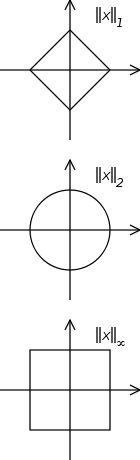
\includegraphics[scale=.3]{140px-Vector_norms.png}
\caption{``Discos''  de radio 1 en diferentes normas. Es decir $\vb\in \R^2$ tales que $\|\vb\|=1$.}
\end{figure}
\begin{ej}
 Examinando los gráficos de las curvas de
nivel\footnote{Las curvas en las cuales la norma respectiva permanece constante.} de las normas$-p$ se puede intuir que  $\lim_{p\to +\infty}\|\vb\|_p=\|\vb\|_\infty$. De una demostración de este hecho.
\end{ej}
\begin{figure}
 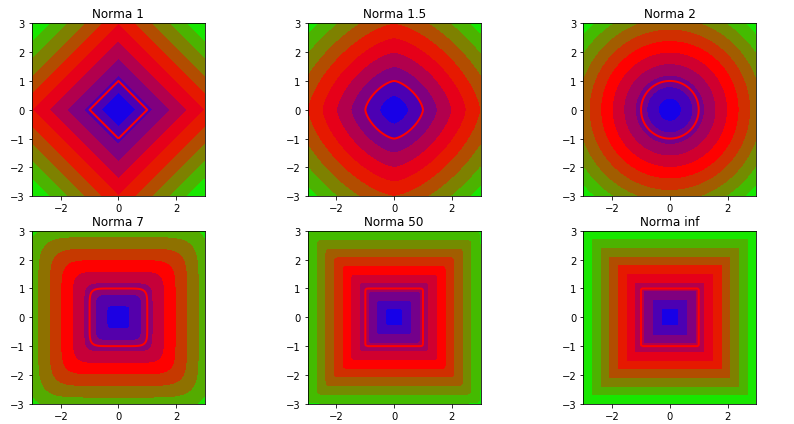
\includegraphics[scale=.4]{nivelNormas.png}
\caption{Curvas de nivel de diferentes normas$-p$.}
\end{figure}
\begin{aplicacion}
Para entender la diferencia entre las distintas normas, analizamos el siguiente ejercicio: Hallar gr\'aficamente el punto del plano de norma igual a 1 que maximiza la funci\'on $f(x,y) = 2y + x$. Para resolverlo, graficamos en el plano todos los puntos para los cuales $f$ tiene un valor fijo. Por ejemplo, los puntos para los cuales $f(x,y) = 3$ se encuentran en una recta que pasa por el punto $(3,0)$ y tiene pendiente $-1/2$. Si aumentamos o disminuimos este valor fijo, obtendremos una recta paralela a la anterior desplazada hacia la derecha o izquierda respectivamente.

Por lo tanto, para resolver el problema, desplazamos la recta que trazamos hacia la izquierda hasta que toque a alguno de los puntos de norma 1.
Concluimos que en el caso de la norma-1 este punto es el punto $(1,0)$, para la norma infinito este punto es el punto $(1,1)$ y para la norma 2, este punto es un punto en el arco del primer cuadrante.

En general, al maximizar o minimizar la norma-1 de una función, obtendremos puntos con varias coordenadas nulas, mientras que al minimazar la norma-2 encontraremos puntos con coordenadas no nulas de valor menor que las de la norma-1. Dependiendo la aplicación resultará m\'as \'util una u otra de las normas.
\end{aplicacion}
Para nosotros va a ser relevante medir \emph{errores} en espacios vectoriales, para ello recordemos que dados $\ub,\vb\in \R^n$
$\|\ub-\vb\|_2$ da la distancia entre ellos. En ocasiones, sin embargo, vamos a notar que es mas sencillo trabajar con una norma diferente a la norma-$2$, por lo que resulta natural ver que relación hay entre las diferentes normas-$p$. Puede probarse muy fácilmente lo siguiente.
\begin{ej}
Verificar que para todo $\xb\in \K^n$
\begin{enumerate}
\item $\|\xb\|_2 \le \|\xb\|_1 \le \sqrt{n} \|\xb\|_2$
\item $\|\xb\|_\infty \le \|\xb\|_2 \le \sqrt{n} \|\xb\|_\infty$
\item $\|\xb\|_\infty \le \|\xb\|_1 \le n \|\xb\|_\infty$
\end{enumerate}
\end{ej}
Ese resultado es un caso particular de uno mucho mas general. Primero definamos \emph{equivalencia de normas}.
\tccdefi
\begin{defi}
 Sean $\|\cdot\|$ y $\|\cdot\|_{*}$ dos normas en un $\K$-espacio vectorial $V$. Decimos que son equivalentes si existen dos constantes $0<c,C$ tales que para todo $\xb\in V$
 $$
 c\|\xb\|_* \le \|\xb\| \le C \|\xb\|_*
 $$
\end{defi}
\etcc
Vale lo siguiente,
\begin{prop}
\label{prop:equivnorm}
 En un $\K$-espacio vectorial de dimensión finita todas la normas son equivalentes\footnote{Las constantes que relacionan las normas dependen de la dimensión $n$, típicamente se deterioran si $n\to \infty$}.
\end{prop}
Este resultado nos es útil en muchos contextos.  Veamos primero la siguiente definición.
\tccdefi
\begin{defi}
Decimos que una sucesi\'on de vectores $\{v_n\}_{n \in \N}$ converge bajo una norma $\|\cdot\|$ a un vector $v$ si
$$
\|v_n - v\| \rightarrow 0 \quad \text{ cuando } n \rightarrow \infty.
$$
\end{defi}
\etcc
Como consecuencia de la Proposición \ref{prop:equivnorm}, la convergencia en una norma cualquiera implica la convergencia en todas las normas.

\section{Producto Interno}
\tccdefi
\begin{defi}
Dados dos vectores $\ub, \vb \in \K^n$ definimos\footnote{Recordemos que asociamos los vectores con las matrices columna.} el producto interno (canónico) por la fórmula\footnote{En muchos casos se suele conjugar los coeficientes del $\vb$ en la sumatoria en vez de los de $\ub$  en la definición de $\langle \ub,\vb\rangle$. Para nuestros intereses no cambia en absoluto la definición utilizada que por lo demas coinciden sobre $\R$.} $$
\langle \ub, \vb \rangle = \ub^*\vb\in \K,
$$
es decir
$$
\langle \ub, \vb \rangle=\overline{u_1} v_1 + \overline{u_2} v_2 + \dots + \overline{u_n} v_n = \sum_{i=1}^{n} \overline{u_i}v_i.
$$
\end{defi}
\etcc
Tenemos las siguientes propiedades inmediatas.

\tcc
\begin{rem}
\label{obs:interno}
Notar que para $\xb,\yb,\zb \in \K^n$, $\wb\in \K^m$ $a,b \in \K$,  $\Ab\in \K^{n \times m}$, resulta

\begin{enumerate}
\item   $\langle \xb, \yb \rangle= \overline{\langle \yb, \xb \rangle}$,
\item   $\langle \xb, a\yb + b\zb \rangle = a \langle \xb, \yb \rangle + b \langle \xb, \zb \rangle$,  y $\langle a\yb + b\zb,\xb \rangle = \overline{a} \langle \yb, \xb \rangle + \overline{b} \langle \zb, \xb \rangle$.
\item  $\langle \Ab\wb, \xb \rangle = \langle  \wb,\Ab^* \xb \rangle$\footnote{Puesto que $\langle \Ab\wb, \xb \rangle = (\Ab\wb)^*\xb=\wb^*\Ab^*\xb= \langle  \wb,\Ab^* \xb \rangle$.}
  \item $\langle a\xb, a\yb \rangle = \overline{a}a \langle \xb, \yb \rangle=|a|^2 \langle \xb, \yb \rangle$.
\item  Utilizando el producto interno, la norma-$2$ de un vector se puede definir por la fórmula $\|\vb\| = \sqrt{\langle \vb, \vb\rangle}$.
\item La desigualdad de Cauchy-Schwarz se escribe
$|\langle \vb,\wb\rangle|\le \|\vb\|_2\|\wb\|_2,$
 \end{enumerate}
\end{rem}
\etcc

\begin{ejemplo}
$\langle \xb + \yb, \xb + \yb\rangle = \langle \xb, \xb + \yb\rangle + \langle \yb, \xb + \yb\rangle = \langle \xb, \xb \rangle + \langle \xb, \yb \rangle + \langle \yb, \xb \rangle + \langle \yb, \yb\rangle = \|\xb\|^2 + 2\langle \xb, \yb \rangle + \|\yb\|^2$
\end{ejemplo}
Sean $\xb,\yb\in \R^2$, $\xb\neq \cero\neq \yb$, $\xb=(a_1,a_2)$, $\yb=(b_1,b_2)$.   Podemos escribir $\xb=\|\xb\|\frac{\xb}{\|\xb\|}$ y como $ \frac{\xb}{\|\xb\|}$ está en el círculo de radio $1$ vemos que existe un único $\alpha$, $0\le \alpha<2\pi$ tal que
$ \frac{\xb}{\|\xb\|}=(\cos(\alpha),\sen(\alpha))$. Es decir, $\xb=\|\xb\|_2(\cos(\alpha),\sen(\alpha))$. Análogamente, podemos escribir $\yb=\|\yb\|_2(\cos(\beta),\sin(\beta))$ y en particular\footnote{Recordar: $
cos(\alpha +\beta)=cos(\alpha)cos(\beta)-sen(\alpha)sen(\beta),
$
$
sen(\alpha +\beta)=sen(\alpha)cos(\beta)+cos(\alpha)sen(\beta).
$
}
$$
\langle \xb,\yb\rangle= \|\xb\|_2\|\yb\|_2\left(\cos(\alpha)\cos(\beta)+\sen(\alpha)\sen(\beta)\right)=\|\vb\|_2\|\wb\|_2\cos(\alpha-\beta),
$$
lo que dice que puede escribirse
\begin{equation}
 \label{eq:calculodeAng}
\cos(\theta)=\frac{\langle \xb,\yb\rangle}{\|\vb\|_2\|\wb\|_2},
\end{equation}
con $\theta$ el ángulo\footnote{Considerando que $\cos(\mu)=\cos(2\pi-\mu)$ siempre puede elegirse $0\le \theta < \pi$.} entre $\xb$ y $\yb$.
\begin{center}
 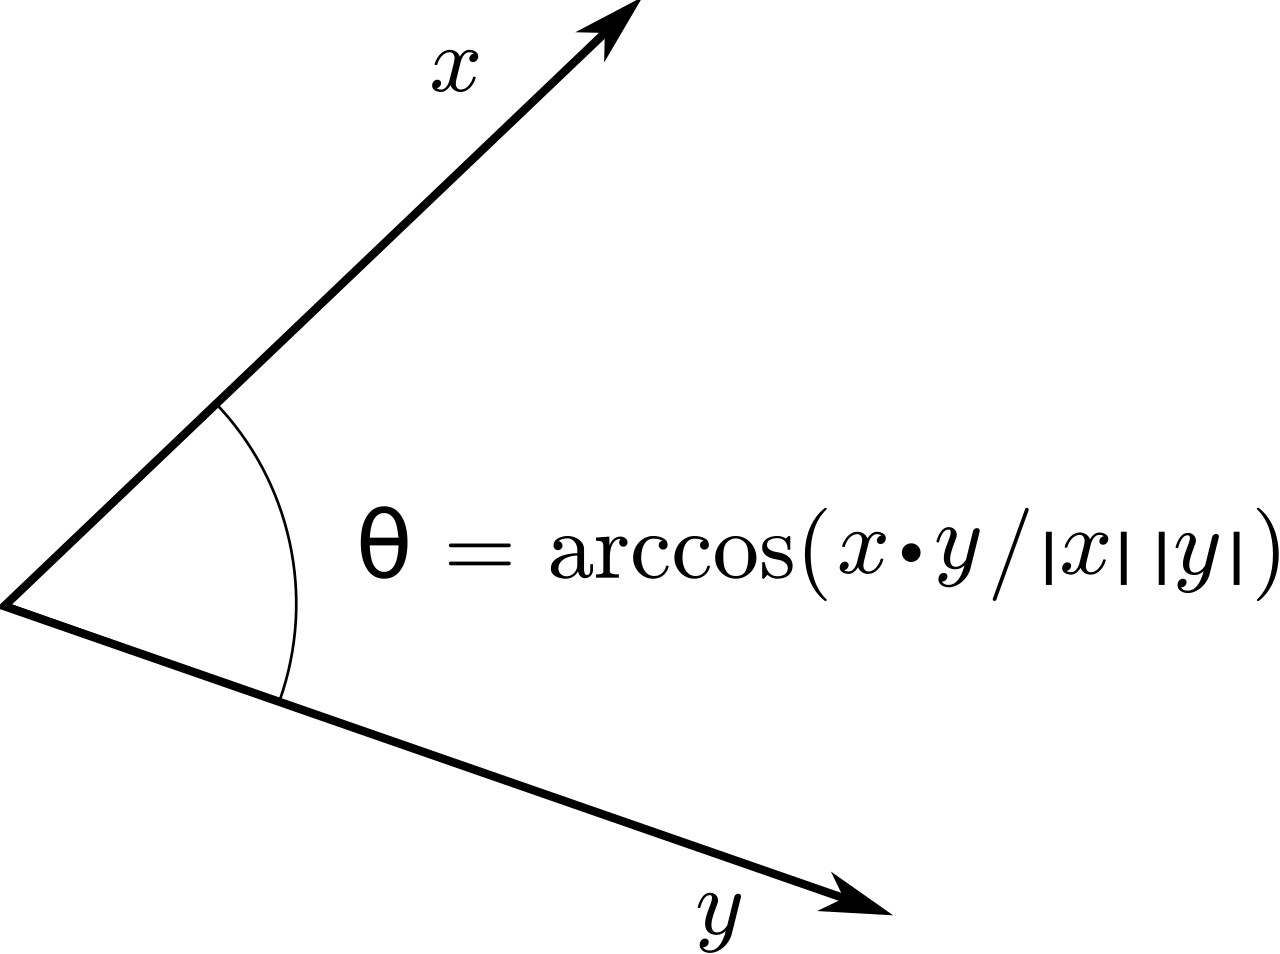
\includegraphics[scale=0.1]{angulo.png}
\end{center}
En $\Rn$ ocurre lo mismo. Ya que $-1\le\frac{\langle \xb, \yb\rangle}{\|\xb\|\|\yb\|}\le 1$, (ver (6) de la Observación \ref{obs:interno}) se define el ángulo $\theta$ entre $\xb$ e $\yb$ a través de \eqref{eq:calculodeAng}.



\tcc
Las normas nos han permitido incorporar al \emph{álgebra} (el espacio vectorial) el concepto de distancia, que  nos permitirá introducir la noción de convergencia y una forma de medir errores.  El producto escalar, por su parte, nos permite trabajar con ángulos. En particular con la idea de perpendicularidad u ortogonalidad que resulta  fundamental en el desarrollo de algoritmos estables.
\etcc
De \eqref{eq:calculodeAng} vemos que $\theta=\pi/2$ si y solo si $\vb^*\wb=0$, de ahí la siguiente definición que la extendemos a los complejos.
\tccdefi
\begin{defi}
 Dados $\vb,\wb\in\K^n$, no nulos. Decimos que son ortogonales sí y solo sí  $\vb^*\wb=\langle \vb,\wb\rangle=0.$ En este caso también usaremos la notación $\vb\perp \wb$.
\end{defi}
\etcc
\tccdefi
\begin{defi}
 Una colección de vectores  $\{\vb_i\}_{1\le i\le k}\subset \K^{n}$ se dice \emph{ortogonal} si $\langle \vb_i,\vb_j\rangle =\delta_i^j$. Si además $\|\vb_i\|_2=1$ para todo $i\le i\le k$ decimos que el conjunto es \emph{ortonormal.}
\end{defi}
\etcc
Los conjuntos ortogonales tienen muchas propiedades que pueden explotarse, tanto teóricamente como en la práctica. Veamos una de ellas de importancia fundamental. Sea $\mathcal{B}=\{\vb\}_{1\le i\le n}\subset \K^n$ una \emph{base} ortonormal de $\K^n$. Dado $\wb\in \K^n$ queremos conocer las coordenadas de $\wb$ en la base $\mathcal{B}$. Esto se reduce a hallar los  $\{\alpha_i\}_{1\le i\le n}\subset \K$ tales que
\begin{equation}
\label{eq:escritura_ort}
\wb=\sum_{i=1}^n\alpha_i\vb_i,
\end{equation}
que como sabemos implica resolver un sistema de $n\times n$. Sin embargo en este caso particular, vemos que para cada $1\le j\le n$ el producto escalar
\begin{equation}
\label{eq:proyecciones}
\vb_j^*\wb=\sum_{i=1}^n\alpha_i\vb_j^*\vb_i=\alpha_j,
\end{equation}
permite ``despejar'' $\alpha_i$ por el módico costo de un producto escalar\footnote{Esto es $2n-1$ operaciones, $n$ productos y $n-1$ sumas.}
Desde el punto de vista matricial, sea $\Qb\in \K^{n\times n}$, que tiene por columnas los $\vb_i$. Resulta que el problema anterior se puede escribir de modo matricial
$$
\wb=\Qb\begin{pmatrix}
        \alpha_1\\
        \vdots\\
        \alpha_n
       \end{pmatrix},
$$
y de la expresión de mas arriba vemos que
$$
\Qb^*\wb=\begin{pmatrix}
        \alpha_1\\
        \vdots\\
        \alpha_n
       \end{pmatrix}.
$$
Esto no expresa mas que el hecho de que invertir $\Qb$ se reduce a conjugar (trasponer si $\K=\R$) lo que a su vez es inmediato considerando que sus columnas son ortonomales\footnote{El costo total de resolver el sistema es $n(2n-1)\sim O(2n^2)$ operaciones. } y así
$$
[\Qb^*\Qb]_{ij}=\vb_i^*\vb_j=\delta_i^j.
$$
Estas matrices tienen un nombre particular.
\begin{defi}
\label{def:de_unitaria}
 Una matriz $\Qb\in \K^{n\times n}$ se dice \emph{unitaria} (suele llamarse \emph{ortogonal} cuando $\K=\R$) si
 $\Qb^*\Qb=\Ib$ ($\Qb^T\Qb=\Ib$ si $\K=\R$).
\end{defi}
\begin{rem}
$\Qb$ es unitaria (resp. ortogonal) si y solo si $\Qb^*$ es unitaria (resp. ortogonal).
\end{rem}
Estudiemos ahora el problema de calcular la proyección \emph{ortogonal} de un vector $\wb$ sobre la recta generada por otro vector $\vb\neq \cero$ (ver Figura \ref{fig:proyusobrev}).
Es decir, que buscamos un vector $\beta\vb$
 tal que $(\beta\vb -\wb)\perp \vb$, esto equivale a
 $(\beta\vb -\wb)^* \vb=0$, lo que indica que $\overline{\beta}=\frac{\wb^*\vb}{\|\vb\|_2^2}$, es decir
 $$
 \beta=\frac{\vb^*\wb}{\|\vb\|_2^2}.
 $$
 Si $\|\vb\|=1$ la expresión coincide con la de los $\alpha$ calculados en \eqref{eq:proyecciones}, lo que nos da una interpretación alternativa de \eqref{eq:escritura_ort}. Esto es, llamando
 $\Pb_{\vb}(\wb)$ a la proyección ortogonal de $\wb$ sobre el subespacio generado por $\vb$, vemos que
\begin{equation}
 \label{eq:proy_forma1}
 \Pb_{\vb}(\wb)=\frac{\vb^*\wb}{\|\vb\|_2^2}\vb,
\end{equation}
y en particular \eqref{eq:escritura_ort} toma la forma
 $$
 \wb=\sum_{1\le i\le n}\Pb_{\vb_i}(\wb).
 $$

\begin{figure}
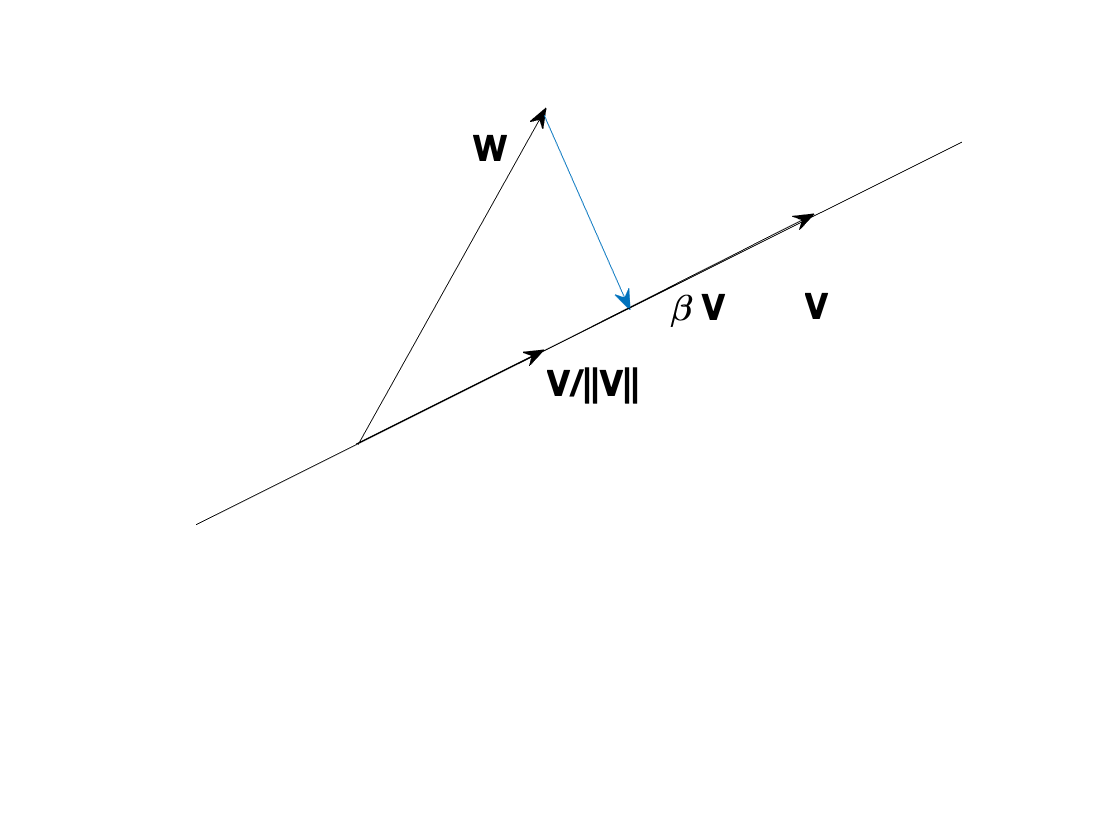
\includegraphics[scale=0.25]{proywsobrev.png}
\caption{Proyección de $\wb$ sobre la recta generada por $\vb$.}
 \label{fig:proyusobrev}
\end{figure}

\tcc
De los argumentos previos vemos que \emph{en una base ortonormal}, las proyecciones ortogonales de un vector $\wb$ sobre los elementos de la base nos dan sus coordenadas en esa base. Eso  es justamente a lo que estamos acostumbrados en la base can\'onica.
\etcc
Otro hecho de gran importancia es la generalización del teorema de Pitágoras en cualquier dimensión si tenemos una base ortonormal. Esto es, de la expresión \eqref{eq:escritura_ort}, tenemos que el cuadrado de la longitud de $\wb$ (el cuadrado de la ``hipotenusa'') es, por un lado
$$\|\wb\|^2_2=\wb^*\wb$$ y por el otro
$$
(\sum_{i=1}^n\alpha_i\vb_i)^*(\sum_{i=1}^n\alpha_i\vb_i)=(\sum_{i=1}^n\overline{\alpha_i}\vb_i^*)(\sum_{i=1}^n\alpha_i\vb_i)=
\sum_{i,j=1}^n\overline{\alpha_j}\alpha_i\vb_j^*\vb_i=\sum_{i=1}^n\overline{\alpha_i}\alpha_i=\sum_{i=1}^n|\alpha_i|^2,
$$
es decir el cuadrado de la suma de las longitudes de las coordenadas (los ``catetos'').
Para resaltar este hecho que usaremos en lo sucesivo, lo recuadramos,
\tcc
\begin{rem}
\label{obs:pitagoras}
En toda base ortonormal $\mathcal{B}=\{\vb_1,\cdots,\vb_n\}$, si
$$
\wb=\sum_{i=1}^n\alpha_i\vb_i,
$$
entonces
$$
\|\wb\|^2=\sum_{i=1}^n|\alpha_i|^2.
$$
\end{rem}
\etcc
Mas adelante (Sección \ref{sec:proyectores}) volveremos sobre el tema de las proyecciones.

Para finalizar la sección de producto interno definimos

\tccdefi \begin{defi}
 Una matriz $\Ab\in \Cnn$ se dice \emph{Hermitiana} si $\Ab=\Ab^*$. En el caso de que $\Ab\in \Rnn$, $\Ab$ se dice \emph{simétrica}.
\end{defi}
\etcc
Si $\Ab\in \Knn$ es Hermitiana, entonces, para todo $\vb\in \Kn$, $\vb^*\Ab\vb\in \R$. En efecto, por un lado, debido a las dimensiones de los elementos que aparecen en el producto, se tiene  $z=\vb^*\Ab\vb\in \K$, por otro lado puesto que
$$\overline{\vb^*\Ab\vb}=(\vb^*\Ab\vb)^*=\vb^*\Ab^*(\vb^*)^*=\vb^*\Ab\vb,$$
resulta de la primera y ultima expresión de la cadena de igualdades que $\overline{z}=z$, es decir $z\in \R$.

\tccdefi
\begin{defi}
\label{def:positiva}
 Una matriz $\Ab\in \Cnn$ ($\Ab\in \Rnn$)  se dice \emph{definida positiva} si es Hermitiana (simétrica) y además $\vb^*\Ab\vb>0$ para todo $\vb\neq 0$.  Si por otro lado $\vb^*\Ab\vb\ge0$ para todo $\vb$, la matriz se dice \emph{semi definida} positiva.
\end{defi}
\end{tcolorbox}


\section{Normas de matrices}
Dada una matriz $A \in \K^{n \times m}$, se la puede pensar pensar como un vector de $\K^{nm}$ y en consecuencia se aplicaría a las matrices todo lo que hemos desarrollado para normas vectoriales.  Sin embargo, salvo casos excepcionales\footnote{Como la norma de Frobenius que veremos mas adelante.}, esta normas no son de gran utilidad en el contexto de las matrices. Esto es debido a que nos interesa estudiarlas desde la perspectiva  de las trasformaciones lineales asociadas. Por esta razón se introducen las normas subordinadas.

Dada una matriz $\Ab \in \K^{n \times m}$, y un par de normas vectoriales $\|\cdot\|_n,\|\cdot\|_m$ en $\K^n$ y $\K^m$ respectivamente, definimos
$$
\|\Ab\|_{n,m} = \max_{\cero \neq \xb \in \K^m} \frac{\|\Ab\xb\|_n}{\|\xb\|_m} = \max_{\xb \in \K^m, \|\xb\|_m = 1} \|\Ab\xb\|_n.
$$
Un caso usual en este curso es que la matriz sea cuadrada $\Ab \in \K^{n \times m}$ y en ese caso usamos una sola norma vectorial $\|\cdot\|$
\tccdefi
\begin{equation}
 \label{eq:defidenormaA}
\|\Ab\| = \max_{\cero \neq \xb \in \K^m} \frac{\|\Ab\xb\|}{\|\xb\|} = \max_{\xb \in \K^m, \|\xb\| = 1} \|\Ab\xb\|.
\end{equation}
\etcc

Estas normas matriciales se dicen \emph{subordinadas} a la norma vectorial $\|\cdot\|$ que estamos utilizando
en el espacio $\Kn$ . De su definición vemos que  la norma (subordinada) de una matriz mide en qué proporción puede aumentar como máximo la norma de un vector $\xb$ al multiplicarlo por $\Ab$.

\begin{ej}
Sea $\Ab\in \Knn$ y $\|\cdot\|$ una norma en $\Kn$, entonces
 \eqref{eq:defidenormaA} define una norma.
\end{ej}
También resulta inmediato de la definición que para todo $\xb$
\begin{equation}
 \label{eq:acotacionoperador}
\|\Ab\xb\|\le \|\Ab\|\|\xb\|.
\end{equation}
De aquí se obtiene la siguiente propiedad. Para todo par de matrices\footnote{Como se desprende de la cuenta,  también vale para matrices rectangulares para las que esté definido el producto.} $\Ab, \Bb\in \K^n$, y toda \emph{norma subordinada}
\begin{equation}
 \label{eq:prodnormas}
\|\Ab\Bb\|\le \|\Ab\|\|\Bb\|.
\end{equation}
En efecto,
dos aplicaciones sucesivas de \eqref{eq:acotacionoperador} da
$$
 \|\Ab\Bb\|=\max_{\|\xb\|=1}
\|\Ab\Bb\xb\|\le \max_{\|\xb\|=1}
\|\Ab\|\|\Bb\xb\|\le \max_{\|\xb\|=1}\|\Ab\|\|\Bb\|\|\xb\|=\|\Ab\|\|\Bb\|,$$
que prueba \eqref{eq:prodnormas}.
Aplicando sucesivamente \eqref{eq:prodnormas}, vemos que para toda matriz cuadrada y para todo $k\in\N$, vale
\begin{equation}
 \label{eq:normasypotencias}
\|\Ab^k\|\le \|\Ab\|^k.
 \end{equation}

En algunos pocos casos es posible calcular explícitamente la expresión de $\|\Ab\|$.

\begin{ejemplo}
Consideremos en $\K^n$ la norma $\|\cdot\|_\infty$. Para $\Ab\in \Knn$ se tiene\footnote{También vale la demostración en el caso de matrices rectangulares.}
\tcc
$$
 \|\Ab\|_\infty=\max_{1\le i\le n}\{\sum_{j=1}^{n} |a_{ij}|\}.
$$
\etcc
\begin{proof}
 Lo vemos para $\K=\R$. Debemos calcular
$$\|\Ab\|_\infty =
\max_{\xb \in \R^n, \|\xb\|_\infty = 1} \|\Ab\xb\|_\infty.
 $$
 Llamemos $k$ a la fila donde ser realiza el máximo, es decir
 $$
 \max_{1\le i\le n}\{\sum_{j=1}^{n} |a_{ij}|\}=\sum_{j=1}^{n} |a_{kj}|,
 $$
 (si hay mas de una tomamos cualquiera). Podemos suponer que
 $\sum_{j=1}^{n} |a_{kj}|>0$ de otro modo el resultado es inmediato. Llamemos $\zb$ al vector de los signos de los elementos de esa fila $\zb=(sg(a_{k,1}),\cdots ,sg(a_{k,n})$. Si algún $a_{k,i}=0$ tomamos $sg(a_{k,1})=0$. Como la fila no es nula, $\zb\neq\cero$. Luego $\|\zb\|_\infty=\max_{1\le i\le n}\{|z_i|\}=1$, y  haciendo
 $$
\|\Ab\|_\infty =\max_{\xb \in \R^n, \|\xb\|_\infty = 1} \|\Ab\xb\|_\infty
 \ge \|\Ab\zb\|_\infty\ge \sum_{j=1}^n a_{i,j}sg(a_{i,j})=\sum_{j=1}^n |a_{i,j}|=\max_{1\le i\le n}\{\sum_{j=1}^{n} |a_{ij}|\},
 $$
 lo que prueba una desigualdad. Para a otra desigualdad, sea $\xb\in \R^n$ tal que $\|\xb\|_\infty=1$, luego para todo $1\le j\le n$ $|x_j|\le \|\xb\|_\infty=1$ y entonces, para cualquier elemento $i$ del vector $\Ab\xb$
$$
|[\Ab\xb]_i|=|\sum_{j=1}^na_{i,j}x_j |\le \sum_{j=1}^n|a_{i,j}|\le \max_{1\le i\le n}\{\sum_{j=1}^{n} |a_{ij}|\},
$$
lo que da la otra desigualdad y demuestra el caso $\K=\R$.
El caso $\K=\C$ sale del mismo modo recordando que si $z\in \C$ y $z=|z|e^{i\theta}$, se tiene que $ze^{-i\theta}=|z|$ y $|e^{i\theta}|=1$.
\end{proof}
Análogamente para la norma$-1$ se tiene
\end{ejemplo}

\begin{ejemplo}
Consideremos en $\K^n$ la norma $\|\cdot\|_1$. Para $\Ab\in \Knn$ se tiene\footnote{También vale  en el caso de matrices rectangulares.}
\tcc
$$
 \|\Ab\|_1=\max_{1\le j\le n}\{\sum_{i=1}^{n} |a_{ij}|\}.
$$
\etcc
\end{ejemplo}
Un caso de mucha importancia para nosotros es la norma matricial subordinada a la norma$-2$.
Comencemos calculando un caso elemental: la norma$-2$ de una matriz unitaria/ortogonal (Definición \ref{def:de_unitaria}).
Supongamos que $\Qb\in \Knn$ y $\Qb^*\Qb=\Ib$, luego, para todo$\xb\in\Kn$
$$
\|\Qb\xb\|_2^2=(\Qb\xb)^*\Qb\xb=\xb^*\xb=\|\xb\|^2_2,
$$
es decir que
\begin{equation}
\label{eq:isometria}
\|\Qb\xb\|_2=\|\xb\|_2, \, \forall \xb\in \K^n.
\end{equation}
 Vemos que las matrices unitarias son \emph{isometrías}, es decir, no cambian las longitudes. Tampoco cambian los ángulos ya que preservan el producto interno, propiedad que recuadramos por su relevancia
 \tcc
 \begin{equation}
 \label{eq:preservaPI}
\langle \Qb\vb,\Qb\wb \rangle=(\Qb\vb)^*\Qb\wb=\vb^*\wb=\langle \vb,\wb \rangle.
 \end{equation}
\etcc
Estas propiedades definen a los \emph{movimientos rígidos}. De \eqref{eq:isometria}, tenemos
$$
\|\Qb\|_2=\sup_{\xb\neq\cero}\frac{\|\Qb\xb\|_2}{\|\xb\|_2}=1,
$$
lo que les da su nombre a las matrices unitarias.
\begin{ej}Verificar que la matriz
$$
\Ab = \begin{pmatrix}
1 & 0 & 0 \\ 0 & \cos \alpha & -\sin \alpha \\ 0 & \sin \alpha & \cos \alpha
\end{pmatrix}
$$
es una matriz ortogonal para cualquier valor de $\alpha$. Interpretar geométricamente la transformación lineal $\Ab\xb$.
\end{ej}

Para calcular la norma$-2$ de otro tipo de matrices  es necesario trabajar con autovalores y autovectores, tema que desarrollaremos con mas detalle mas adelante, presentando ahora solo los conceptos básicos necesarios para esta sección.

Observemos que si  $\ab\in \K^{1\times 1}$ (es decir pensamos el escalar como una matriz), el efecto que tiene la aplicación lineal $\ab \xb:\K^1\to \K^1$ es de una simple dilatación o contracción (si $\K=\C$ también hay rotaciones). En el caso en que $\Ab\in \K^{n\times n}$ uno espera un coportamiento bastante mas complicado de la aplicación $\Ab\xb$, sin embargo, hasta cierto punto esto no es así.
Ya que trataremos la teoría con mas adelante, hagamos un experimento numérico. Generamos matrices al azar $\Ab\in\R^{2\times 2}$  y graficamos en rojo la imagen -reescalada adecuadamente para ser visualizada en la misma escala- del círculo unitario (graficado en azul) a través de la aplicación $\Ab\xb$. En el gráfico siguiente vemos tres ejemplos
\begin{center}
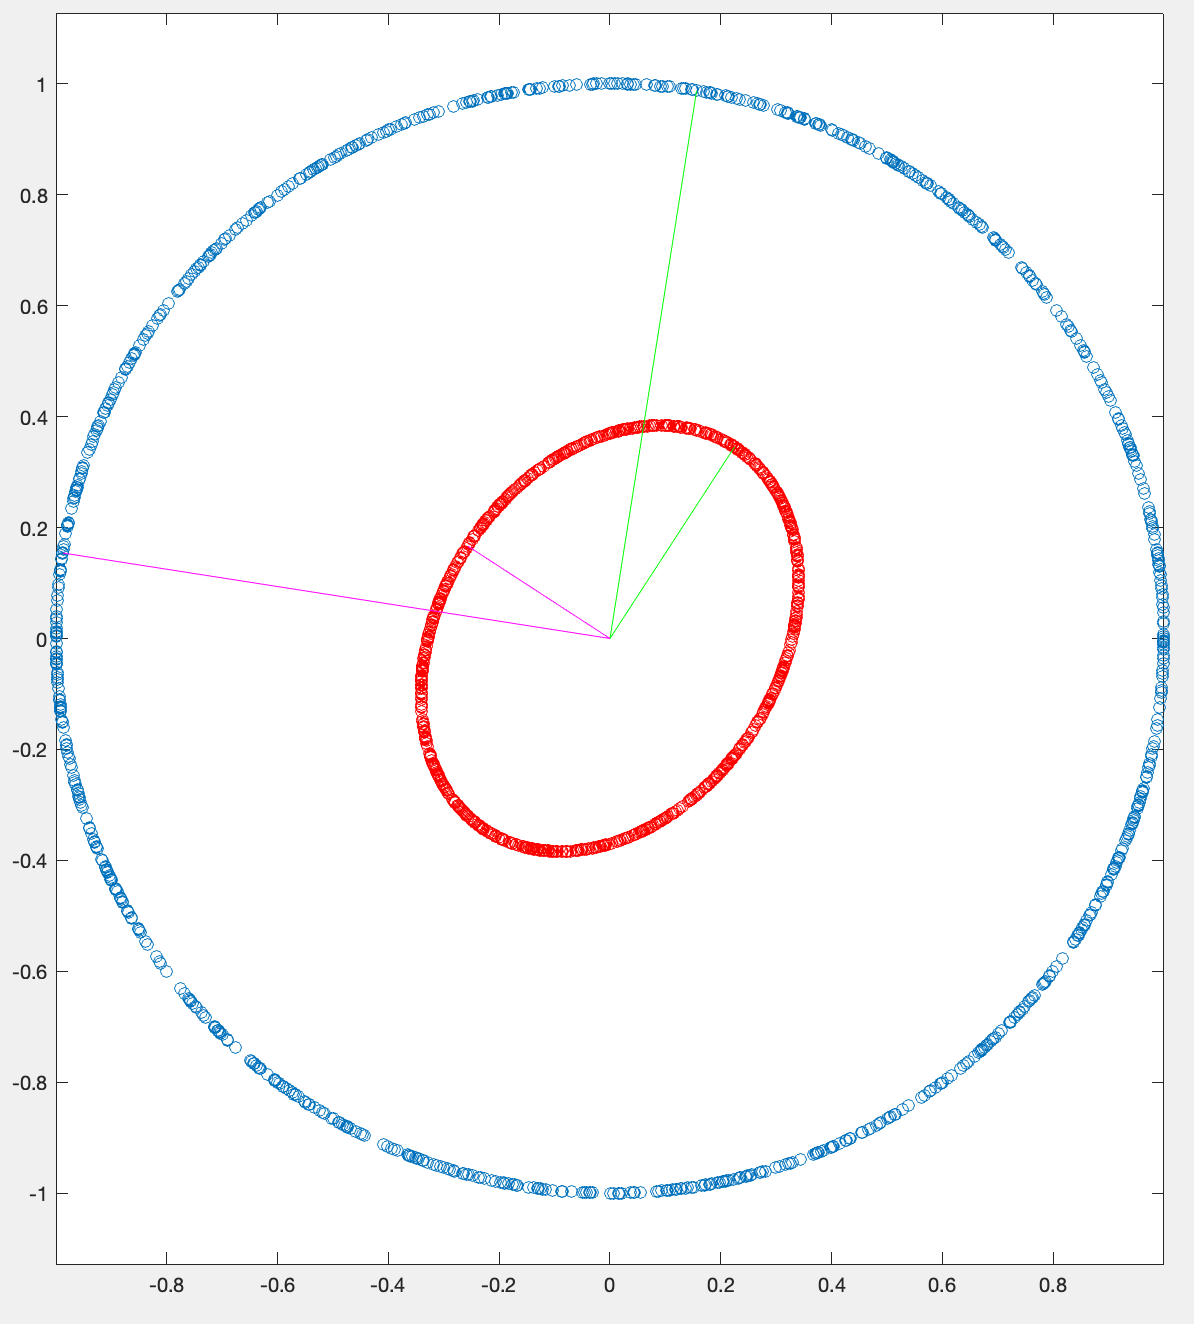
\includegraphics[scale=.2]{rand1.png}
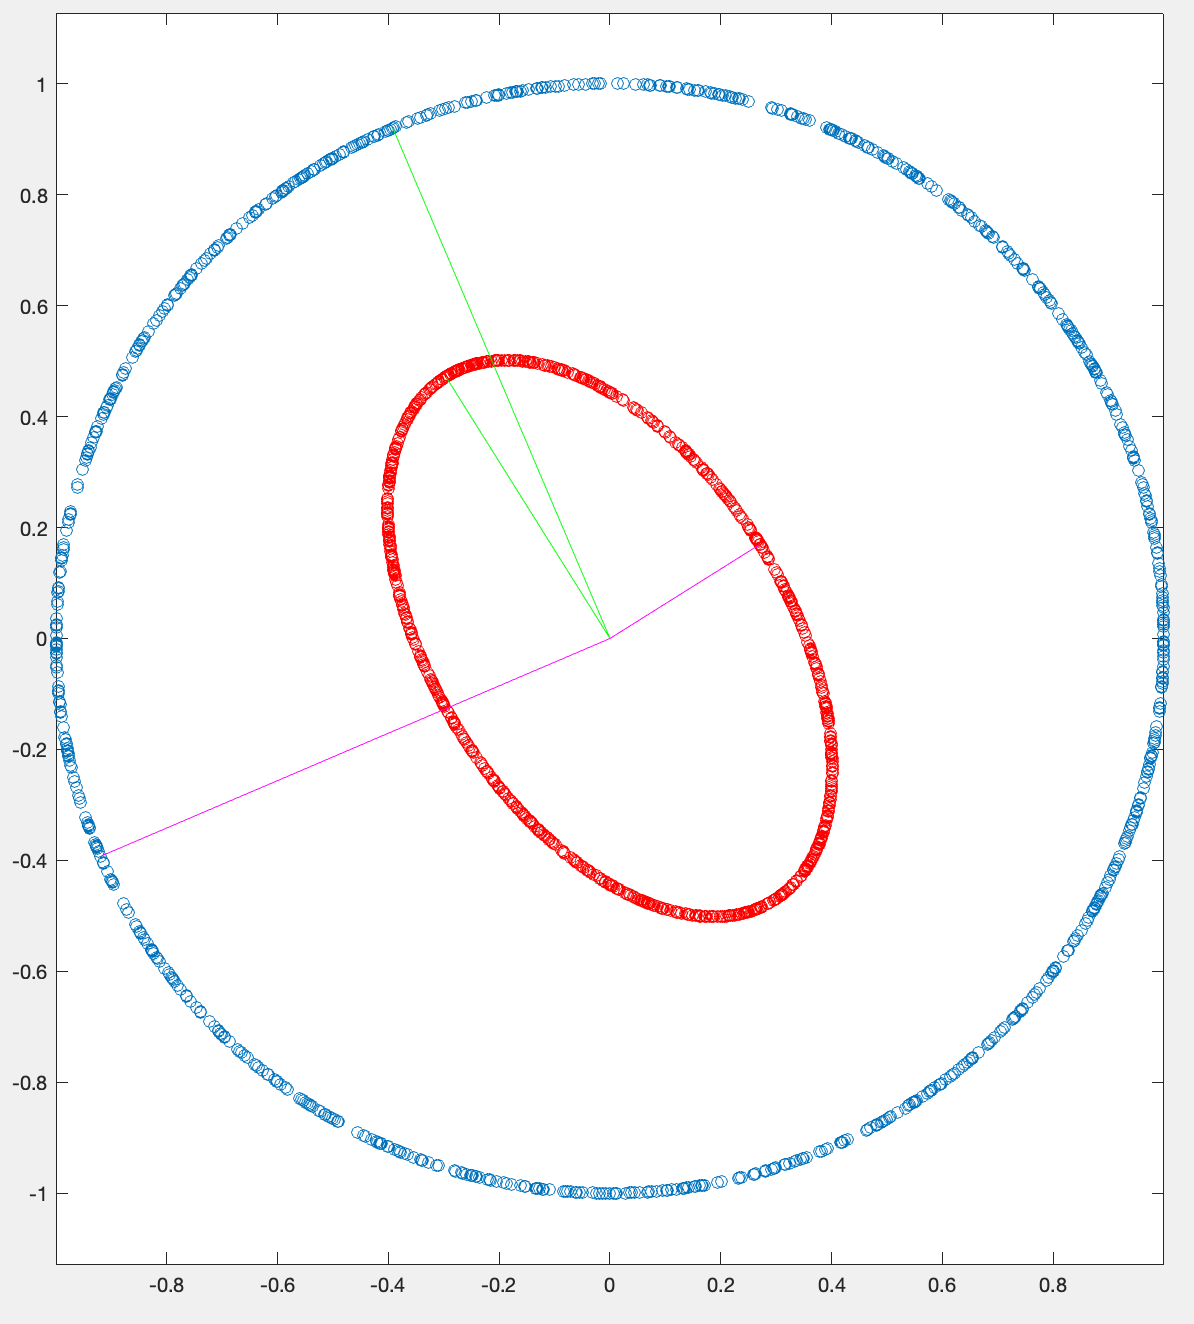
\includegraphics[scale=.2]{rand2.png}
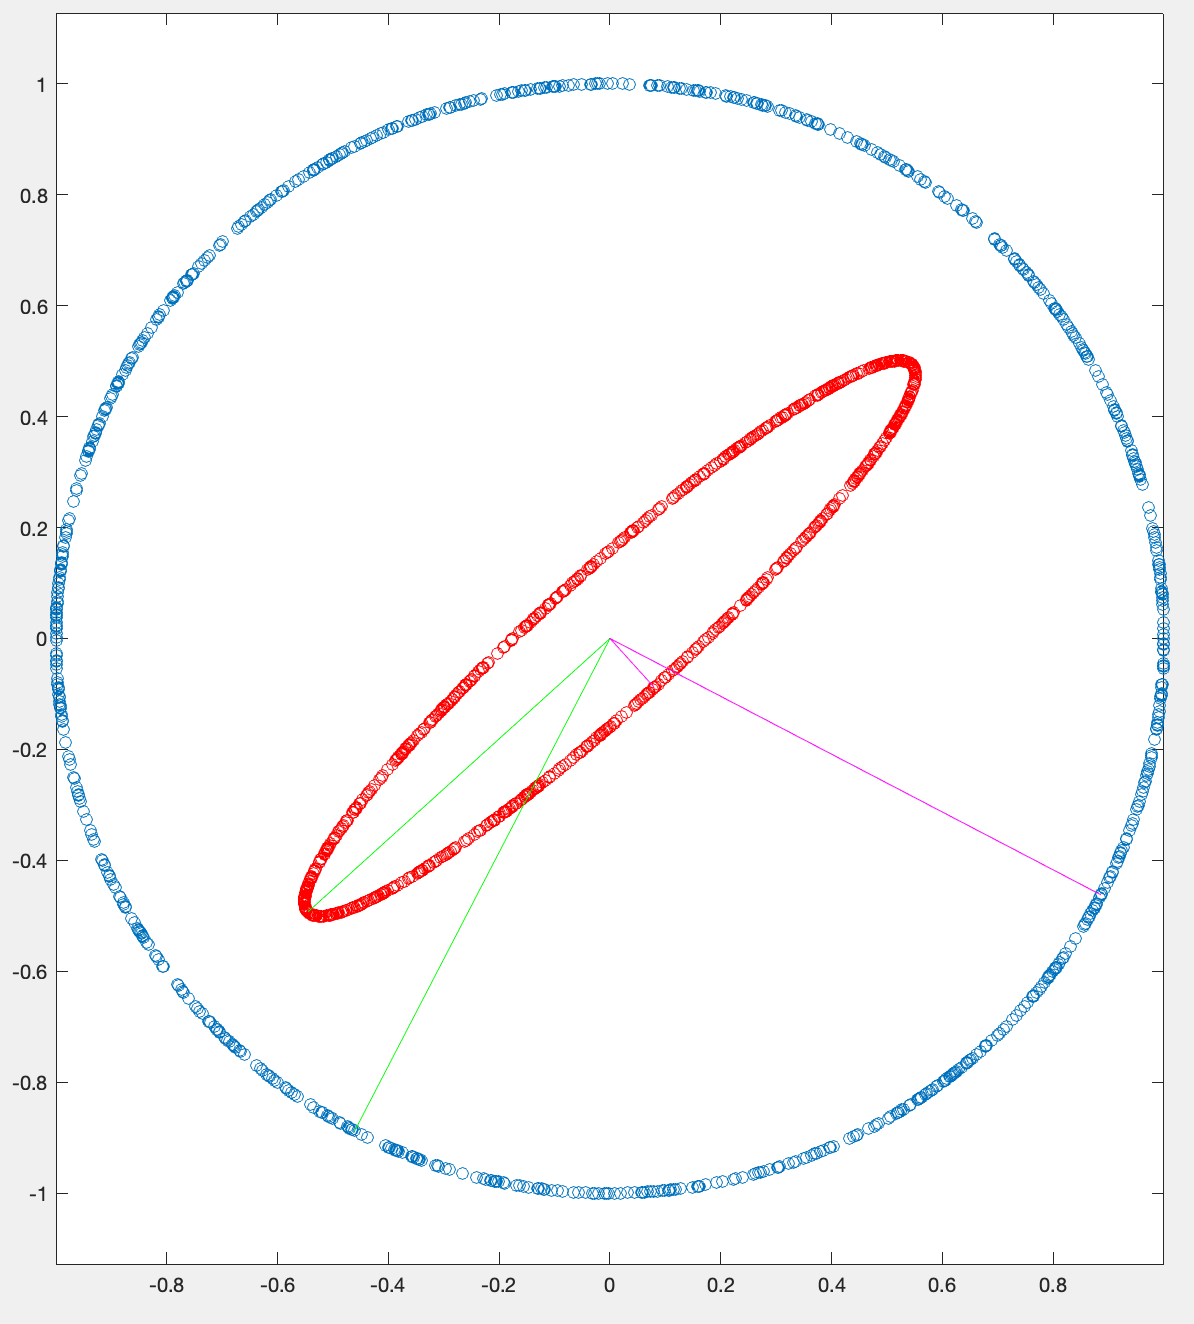
\includegraphics[scale=.2]{rand3.png}
\end{center}
Lo primero que vemos es  que la imágen del círculo es siempre una elipse\footnote{Si la matriz fuera singular obtendríamos  un segmento o un círculo.}. Este es un hecho general que veremos mas adelante. En nuestro experimento además hemos graficado los semiejes de las elipses (con verde el mayor y rosa el menor) que llamaremos $\yb_1$ e $\yb_2$. Por ser semiejes de una elipse sabemos que  $\yb_1\perp \yb_2$. Junto con los semiejes graficamos también sus respectivas preimágenes $\xb_1$ y $\xb_2$ (con el mismo color). El segundo hecho notable para notar es que así como los semiejes, las preimágenes son perpendiculares entre sí. Es decir: existen dos vectores perpendiculares $\xb_1\perp \xb_2$ tales que $\Ab\xb_1=\yb_1\perp \yb_2=\Ab\xb_2$. Esto va dar lugar mas adelante a la descomposición en valores singulares SVD, sin embargo, por ahora vamos a diferir este tema y a realizar el mismo  experimento, pero esta vez con matrices \emph{simétricas}.
\begin{center}
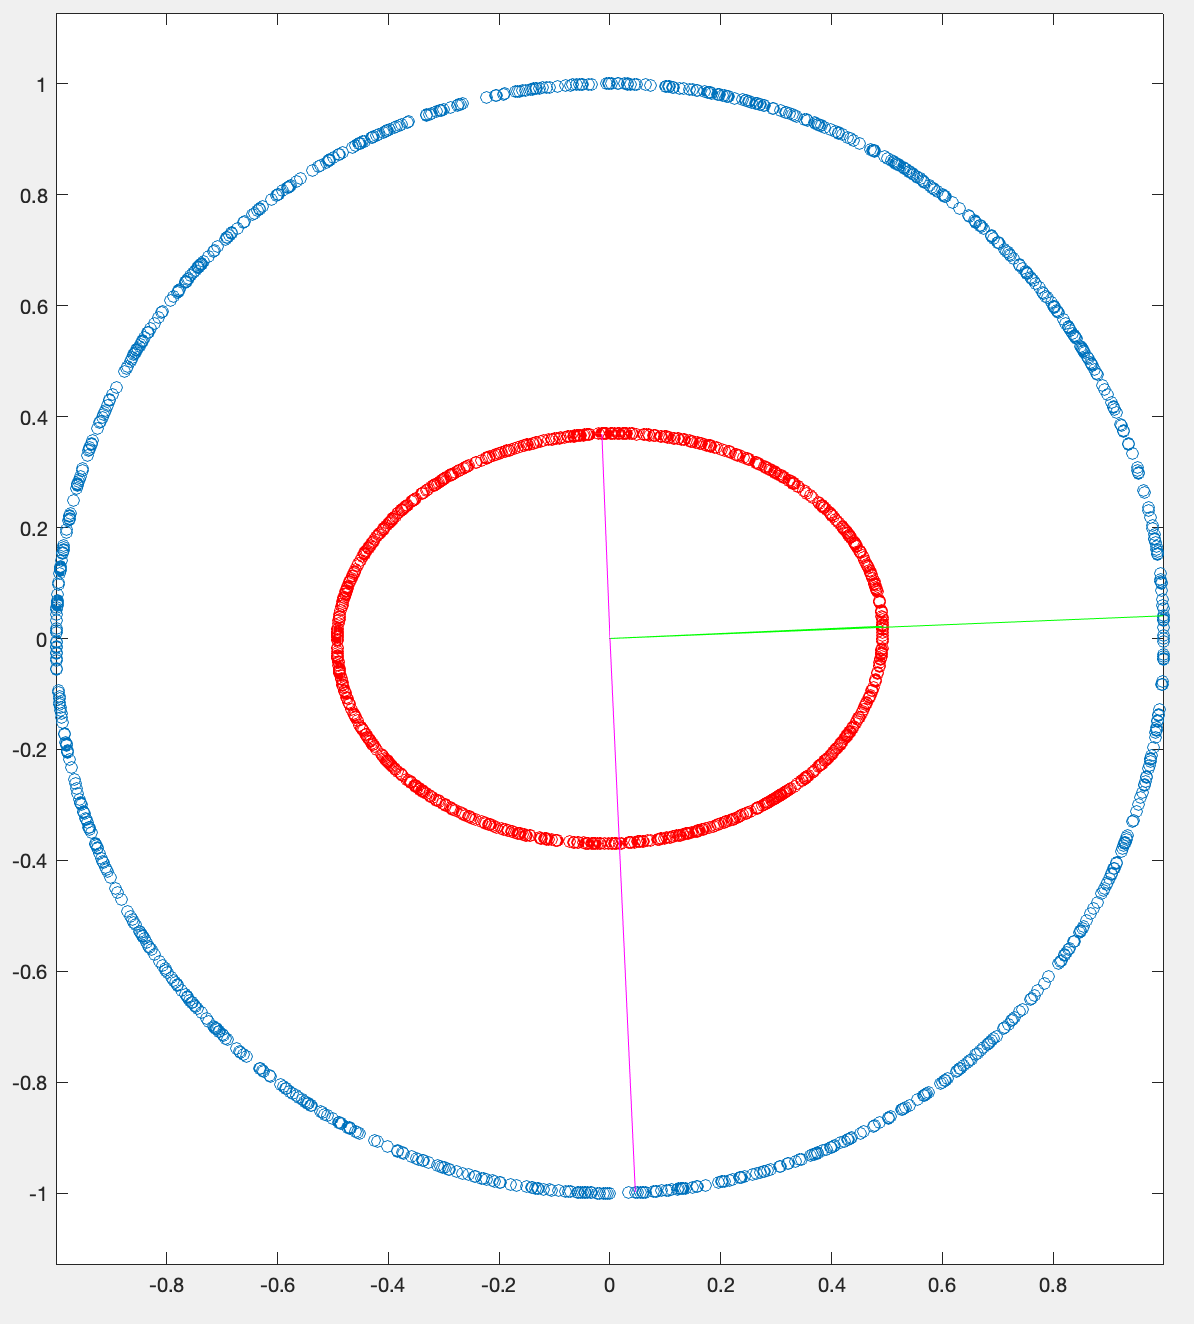
\includegraphics[scale=.2]{randsim1.png}
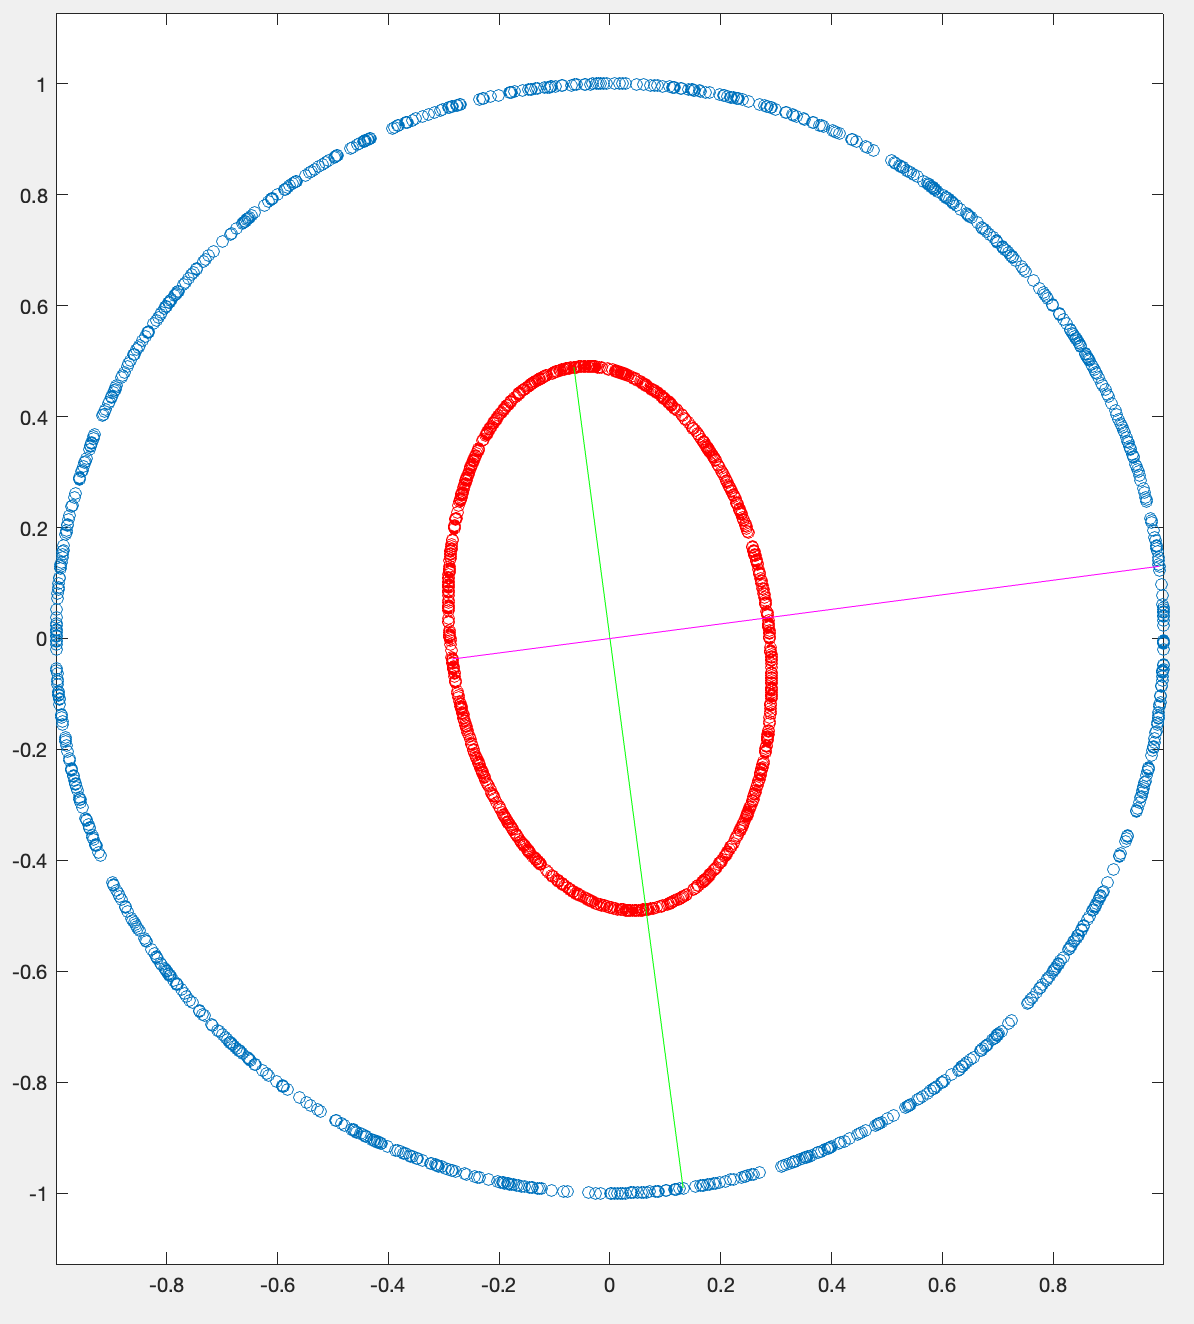
\includegraphics[scale=.2]{randsim2.png}
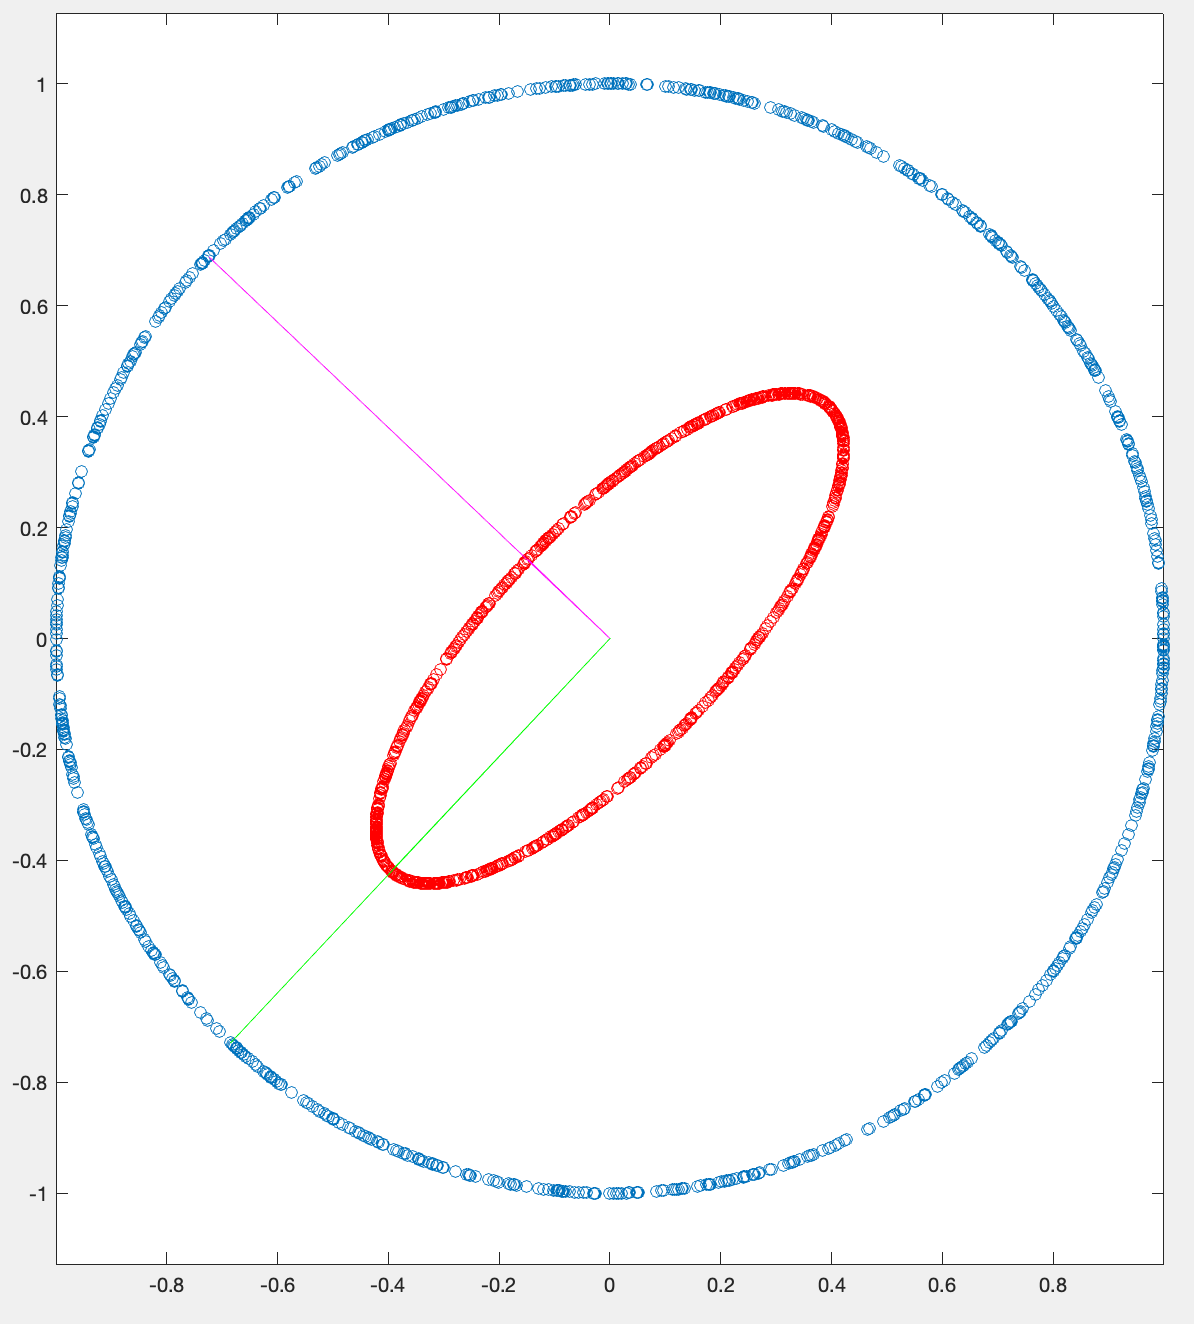
\includegraphics[scale=.2]{randsim3.png}
\end{center}
Lo que vemos ahora es que si $\Ab=\Ab^T$ entonces los semiejes son \emph{multiplos} de sus preimágenes!. Es decir
existen dos vectores perpendiculares $\xb_1\perp \xb_2$ tales que $\Ab\xb_1=\lambda_1\xb_1$ y $\Ab\xb_2=\lambda_2\xb_2$.
Este también es un hecho general que enunciamos luego de la siguiente definición y que probaremos mas adelante.
\tccdefi
\begin{defi}
 Sea $\Ab\in \Cnn$. Un vector $\vb\neq \cero$ tal que $\Ab\vb=\lambda\vb$ para algún $\lambda\in \C$ se llama un \emph{autovector} de $\Ab$ de \emph{autovalor}  $\lambda$.
\end{defi}
\etcc
\begin{rem}
\label{rem:sobreautovalores}Las siguientes observaciones son inmediatas:
\begin{enumerate}
\item $\lambda$ es un autovalor de $\Ab$ si y solo si\footnote{Mas adelante retomaremos el tema de autovalores mas en profundidad.} $\exists \vb\neq \cero$ tal que $(\Ab-\lambda\Ib)\vb=\cero$, y esto ocurre si y solo si $\det(\Ab-\lambda\Ib)=0$, es decir que los autovalores son la raíces de un polinomio de grado $n$, $p(x)=\det(\Ab-x\Ib)$, llamado característico de $\Ab$.

\item Notar que en el caso particular en que $\Ab\in \Rnn$, sus autovalores/autovectores pueden ser complejos.
\item Si $\lambda\neq 0$ entonces $\Ab\vb=\lambda \vb$, si y solo si  $\Ab^{-1}\vb=\lambda^{-1}\vb$. Por lo tanto: $\vb$ autovector de $\Ab$ de autovalor $\lambda\neq 0$ entonces $\vb$ autovector de $\Ab^{-1}$ de autovalor $\lambda^{-1}$.
\end{enumerate}


\end{rem}

\begin{prop}
 Sea $\Ab\in \Rnn$, $\Ab^T=\Ab$, entoces existe una base ortogonal $\mathcal{B}=\{\vb_1,\cdots,\vb_n\}$ de $\Rn$ de autovectores de $\Ab$. Esto es, existen $\{\lambda_1, \lambda_2,\cdots \lambda_n\}\subset \R$ (no necesariamente todos diferentes) tales que:
 \begin{enumerate}
  \item $\vb_i^T\vb_j=\delta_i^j$
  \item $\Ab\vb_i=\lambda_i\vb_i.$
 \end{enumerate}
\end{prop}
\begin{cor}
 Si $\Ab\in \Rnn$, $\Ab^T=\Ab$, entonces existe una base ortogonal $\mathcal{B}=\{\vb_1,\cdots,\vb_n\}$ de $\Rn$ tal que
 $$[\Ab]_{\mathcal{B}}=
 \begin{pmatrix}
  \lambda_1&0&0&\dots&0\\
  0&\lambda_2&0&\cdots &0 \\
  0&0&\lambda_3 &\cdots&0 \\
  \vdots&\vdots & &\ddots&\vdots\\
  0&0&\cdots &&\lambda_n
 \end{pmatrix}
 $$
\end{cor}
Luego de la siguiente definición veremos como calcular la norma$-2$.
\tccdefi
\begin{defi}
 Dada $\Ab\in \Knn$ definimos el radio espectral de $\Ab$ como
 $$
 \rho(\Ab)=\max\{|\lambda|, \, \mbox{con}\, \lambda \,\mbox{autovalor de}\, \Ab\}
 $$
\end{defi}

\etcc
Supongamos que $\Ab\in \Rnn$ es simétrica, sea $\mathcal{B}=\{\vb_1,\cdots,\vb_n\}$ una base ortonormal de autovectores y  $\{\lambda_1, \lambda_2,\cdots \lambda_n\}\subset \R$ los respectivos autovalores.
Sea $\xb\in\R^n$ tal que $\|\xb\|_2=1$, escribiendo $\xb$ en la base $\mathcal{B}$ se tiene
$$
\xb=\sum_{i=1}^n\alpha_i\vb_i,
$$
y por ser $\mathcal{B}$ un conjunto ortonormal tenemos por la Observación \ref{obs:pitagoras}
$$
1=\|\xb\|_2^2=\sum_{i=1}^n\alpha_i^2.
$$
Por otro lado, como $\Ab\xb=\sum_{i=1}^n\alpha_i\lambda_i\vb_i,
$ usando nuevamente la  Observación \ref{obs:pitagoras}
$$
\|\Ab\xb\|_2^2=\sum_{i=1}^n\alpha_i^2\lambda_i^2.
$$
Por lo tanto
$$
\frac{\|\Ab\xb\|^2}{\|\xb\|^2}=\sum_{i=1}^n\alpha_i^2\lambda_i^2\le \rho(\Ab)^2,\qquad, \, \forall \xb, \|\xb\|\le 1
$$
ya que cada $|\lambda_i|\le \rho(\Ab)$. Por otro lado, llamando $j$ a un índice tal que $|\lambda_j|=\rho(\Ab)$ y considerando el vector de norma 1 $\xb=\vb_j$, se tiene
$$
\|\Ab\xb\|^2=|\lambda_j|^2\|\xb\|_2^2=\rho(\Ab)^2.
$$
En definitiva
$$
\sup_{\|\xb\|=1}\|\Ab\xb\|^2=\rho(\Ab)^2.
$$
Esto dice lo que prevíamos en el experimento numérico:
\tcc
Si  $\Ab\in \Rnn$, $\Ab^T=\Ab$ entonces
$$
\|\Ab\|_2=\rho(\Ab).
$$
\etcc
Podemos hacer una cuenta similar para el caso general. En efecto, consideremos ahora $\Ab\in \R^{n\times n}$ no necesariamente simétrica.
Queremos calcular
$$
\sup_{\|\xb\|_2=1}\|\Ab\xb\|_2^2=(\Ab\xb)^T\Ab\xb=\xb^T(\Ab^T\Ab)\xb
$$
Si llamamos $\Mb=\Ab^T\Ab$, resulta simétrica. Consideremos una base  $\mathcal{B}=\{\vb_1,\cdots,\vb_n\}$  ortonormal de autovectores de $\Mb$ y  $\{\lambda_1, \lambda_2,\cdots \lambda_n\}\subset \R$ los respectivos autovalores. Notemos que $\Mb$ es semidefinida positiva (ver Definición \ref{def:positiva}), pues de la ecuación previa se ve que para todo $\xb\in \Rn$
$$
\xb^T\Mb\xb\ge 0,
$$
y en particular se sigue que $\lambda_i\ge 0$ pues si $\vb_i\in \ker(\Ab)$ debe ser $\lambda_i=0$ y en caso contrario
$$
0<\vb_i^T\Mb\vb_i=\vb_i^T\lambda_i\vb_i =\lambda_i.
$$
Con esta información escribimos como antes
$$
\xb=\sum_{i=1}^n\alpha_i\vb_i,
\qquad 1=\|\xb\|_2^2=\sum_{i=1}^n\alpha_i^2, \qquad \Mb\xb=\sum_{i=1}^n\alpha_i\Mb\vb_i=\sum_{i=1}^n\lambda_i\alpha_i\vb_i
$$
de donde por la ortonormalidad de los $\vb_i$
$$
\xb^T\Mb\xb=\sum_{i=1}^n\lambda_i\alpha_i^2.
$$
Luego,
$$
\sup_{\|\xb\|_2=1}\|\Ab\xb\|_2^2=\sup_{\sum_{i=1}^n\alpha_i^2=1}\sum_{i=1}^n\lambda_i\alpha_i^2=\lambda_{max}=\rho(\Mb).
$$
En definitiva tenemos
\tcc
Sea $\Ab\in \Rnn$, entonces\footnote{También vale la demostración escrita mas arriba para el caso de matrices rectangulares.}
$$
\|\Ab\|_2=\sqrt{\rho(\Ab^T\Ab)}.
$$
\etcc
\begin{ej}
 Verifique que de la última expresión se obtiene como caso particular la de las matrices simétricas.
\end{ej}
Otra propiedad importante es la siguiente
\begin{prop}
 \label{prop:infmat=rho}
Sea $\Ab\in\Knn$, entonces
$$
\rho(\Ab)=\inf
\{\|\Ab\|:\, \|\cdot \|\,  \mbox{es una norma subordinada}\}.$$
\end{prop}
\begin{proof}
Solo vamos a probar que  $\rho(\Ab)\le \|\Ab\|$ para cualquier norma subordinada. La otra desigualdad requiere de herramientas que veremos mas adelante.

 Si $\K=\C$ la demostración es mas sencilla.
 Sea $\lambda$ autovalor de $\Ab$ y sea $\|\cdot\|$ una norma matricial en $\Cnn$ subordinada a la norma vectorial\footnote{Usamos la misma notación para ambas normas ya que el contexto indica cuando estamos usando una o la otra.} $\|\cdot\|$. Luego existe $\cero\neq\vb$ autovector de autovalor $\lambda$. Podemos suponer que $\|\vb\|=1$ y entonces
 $$
 \Ab\vb=\lambda\vb,
 $$
 de donde
 $\|\Ab\vb\|\le |\lambda|\|\vb\|=|\lambda|.$ Por lo tanto, para todo $\lambda$ autovalor
 $$
 \|\Ab\|=\sup_{\|\xb\|=1}\|\Ab\xb\|\ge \|\Ab\vb\|\ge |\lambda|.
 $$
 de donde
 $$
 \|\Ab\|\ge \rho(\Ab).
 $$
 Si $\K=\R$ hay un problema si intentamos repetir el argumento previo vemos que funciona perfectamente si $\lambda \in \R$, sin embargo el autovalor y el autovector podrían ser complejos y no tener sentido la expresión $\|\vb\|$ si se trata de una norma en $\Rn$.
 Supongamos entonces que $\lambda=a+ib\in \C$ y escribamos entonces, \footnote{Debemos este argumento a Ariel Lombardi, colega de la UNR.}
$$
\vb=Re(\vb)+iIm(\vb)
$$
y
 $$
 \Ab\vb=(a+ib)(Re(\vb)+iIm(vb)),
 $$
 luego
 $$
 \Ab Re(\vb)=aRe(\vb)-bIm(\vb) \qquad
 \Ab Im(\vb)=bRe(\vb)+bIm(\vb),
 $$
 y entonces
 $$
 \|\Ab Re(\vb)\|_2^2=a^2\|Re(\vb)\|_2^2-2ab\langle Im(\vb),Re(\vb)\rangle+b^2\|Im(\vb)\|_2^2
 $$
 $$
 \|\Ab Im(\vb)\|_2^2=b^2\|Re(\vb)\|_2^2-2ab\langle Im(\vb),Re(\vb)\rangle+a^2\|Im(\vb)\|_2^2
 $$
 sumando miembro a miembro
 $$\|\Ab Re(\vb)\|_2^2+\|\Ab Im(\vb)\|_2^2=(a^2+b^2)\left(\|Re(\vb)\|_2^2+\|Im(\vb)\|_2^2\right)
 $$
 de donde
 $$
 \left(\|Re(\vb)\|_2^2+\|Im(\vb)\|_2^2\right)\|\Ab\|_2^2\ge (a^2+b^2)\left(\|Re(\vb)\|_2^2+\|Im(\vb)\|_2^2\right)
 $$
 y entonces
 $$
 \|\Ab\|_2^2\ge (a^2+b^2)=|\lambda|^2.
 $$
 Es decir -ya que $\lambda$ es arbitrario-
 $$\|\Ab\|_2\ge \rho(\Ab).$$
 Sea ahora $\|\cdot\|$ una norma arbitaria en $\Rn$ y $k\in \N$: por un lado sabemos que\footnote{En realidad vale el igual. Para ver la desigualdad basta notar que si $\lambda$ es autovalor de $ \Ab$ entonces $\lambda^k$ lo es de $\Ab^k$. }
 $\rho(\Ab)^k\le \rho(\Ab^k)
 $ y que además (por Proposición \ref{prop:equivnorm}) existe una constante $C$ -independiente de $k$- tal que $\|\Ab^k\|_2\le C\|\Ab^k\|$. Por lo tanto,
 $$
 \rho(\Ab)^k\le \rho(\Ab^k)\le \|\Ab^k\|_2\le C\|\Ab^k\|\le C\|\Ab\|^k,
 $$
 donde hemos usado \eqref{eq:normasypotencias} en la última desigualdad. Tomando raíz $k-$ésima
 $$
 \rho(\Ab)\le C^{1/k}\|\Ab\|,
 $$
 tomando $k\to \infty$ se obtiene $
 \rho(\Ab)\le \|\Ab\|,
 $
 como queríamos probar.
\end{proof}
Como ya hemos señalado, las normas subordinadas son las mas útiles. Sin embargo la norma euclídea aplicada a matrices -que es no subordinada- tiene importantes aplicaciones y un nombre propio.
\tccdefi
\begin{defi}
 Dada $\Ab\in \K^{n\times m}$ definimos la norma de Frobenius
 $$
 \|\Ab\|_F=\sqrt{\sum_{1\le i\le n}\sum_{i\le j\le m} |a_{i,j}|^2}
 $$
\end{defi}
\etcc
Notar que
$$
\|\Ab\|_F=\sqrt{tr(\Ab^T\Ab)},
$$
donde $tr$ indica el operador traza (la suma de los elementos de la diagonal). Las normas no subordinadas de matrices no suelen cumplir con la desigualdad \eqref{eq:prodnormas}. La norma de Frobenius es una excepción, gracias a la desigualdad de Cauchy-Schwarz. En efecto, dados\footnote{El siguiente argumento vale para matrices rectangulares.}
$\Ab,\Bb\in \K^nn$, consideremos el elemento $i,j$ de la  matriz producto
$$
|[\Ab\Bb]_{i,j}|^2\le |(\sum_{l=1}^n\Ab_{i,l}\Bb_{l,j})|^2\le (\sum_{1=1}^n\Ab_{i,l}^2)(\sum_{1=1}^n\Bb_{l,j}^2),
$$
donde hemos usado la Proposición \ref{prop:CS} en la última desigualdad. Sumando en $i$ y en $j$ se tiene el resultado deseado
$$
\|\Ab\Bb\|_F^2=\sum_{1\le i,j\le n}|[\Ab\Bb]_{i,j}|^2\le\sum_{1\le i\le n}\sum_{1\le j\le n}(\sum_{1=1}^n\Ab_{i,l}^2)(\sum_{1=1}^n\Bb_{l,j}^2)=
\|\Ab\|_F^2\|\Bb\|_F^2.
$$
Esto es
\tcc
$$\|\Ab\Bb\|_F\le \|\Ab\|_F\|\Bb\|_F.$$
\etcc
Cerramos esta sección con propiedades de las normas de matrices unitarias (algunas las hemos ya probado pero las ponemos en recuadro para recordarlas).
De todas la matrices, las unitarias poseen propiedades especiales que las hacen muy favorables para su uso en los algoritmos.
\tcc
\begin{prop}
 \label{prop:unitarias}
 Sea $\Ab\in \K^{n\times m}$, $\Qb\in \Knn$, $\Qb$ unitaria/ortogonal, resulta
 \begin{enumerate}
  \item $\forall \vb\in \Kn$
  $\|\Qb\vb\|_{2}=\|\vb\|_2$
  \item $\|\Qb\|_{2}=1$
  \item $\|\Qb\Ab\|_2=\|\Ab\|_2$
  \item $\|\Qb\Ab\|_F=\|\Ab\|_F$
 \end{enumerate}
\end{prop}
\etcc
\begin{proof} Las propiedades $(1)$ y $(2)$ ya las hemos probado.

Para $(3)$, notemos que por $(1)$ se tiene
 $$\|\Qb\Ab \|_{2}=sup_{\vb, \|\vb\|_2=1}
 \|\Qb\Ab \vb\|_{2}=sup_{\vb, \|\vb\|=1}\|\Ab\vb\|_2=\|\Ab\|_2.
 $$
 Finalmente, para $(4)$ escribimos
 $$
 \|\Qb\Ab\|_F^2=tr((\Qb\Ab)^*(\Qb\Ab))=tr(\Ab^*\Ab)=\|\Ab\|_F^2.
 $$\end{proof}

\section{Números de Máquina}
Los \emph{números de máquina} son aquellos que la máquina puede representar de forma exacta y son, por ende, finitos, limitados por la cantidad de memoria dedicada a su almacenamiento. En este sentido, aún antes de resolver un problema, en la etapa previa de almacenamiento de los datos, ya apacererán errores. El efecto de estos errores sobre la solución del problema o sobre la respuesta que dé un algoritmo a nuestro problema es una cuestión fundamental a la hora de evaluar la calidad de la solución obtenida.


Como hemos mencionado asumimos que trabajamos en $\K$, sin embargo como para almacenar un número complejo basta almacenar su parte real e imaginaria podemos enfocarnos en el caso $\K=\R$.

En general todo número  $x\in \R$ $x\neq 0$, puede representarse en una base $b\in\N$, $b\ge 2$, de la forma\footnote{$(x)_b$ se lee $x$ en la base $b$.}
\begin{equation}
 \label{eq:represbaseb}
(x)_b=sg(x)\bt_k\bt_{k-1}...\bt_0.\bt_{-1}\bt_{-2}...
 \end{equation}
donde los ``dígitos'' verifican $0\le \bt_i\le b-1$, $sg(x)$ el signo de $x$ y donde por convención numeramos los índices para que el punto -o coma- se ubique entre $\bt_0$ y $\bt_1$.

Asumamos que $x$ es positivo para no lidiar con el signo. La representación \eqref{eq:represbaseb} se obtiene de la escritura de $x$ como
$$
x=\bt_kb^k+\bt_{k-1}b^{k-1}+...+\bt_0b^0+\bt_{-1}b^{-1}+\bt_{-2}b^{-2}+...
$$
 que es única si  descartamos los desarrollos infinitos de la forma $\bt_j=b-1$ para todo $j\le l$ con $l\in \Z$ fijo.

 Para aclarar este punto recordemos la expresión  cerrada de la geométrica
$$
\sum_{j=0}^m\beta^j=\frac{\beta^{m+1}-1}{\beta -1},
$$
 válida para $\beta\neq 1$. Notemos que  en caso de tener un $x$ con un desarrollo de la forma
$$
x=\sum_{-\infty}^l(b-1)b^i,
$$
podemos reescribirlo como
$$
x=(b-1)b^{l}
\left(\sum_{-\infty}^0b^i\right)=(b-1)b^l\frac{b}{b-1}=b^{l+1},
$$
lo que indica dos  representaciones alternativas. Como ejemplo si  $l=0$ tenemos
$$
10=(x)_b=(b-1).(b-1)(b-1)(b-1)\cdots
$$

Continuemos asumiendo que $x>0$. El uso del punto \emph{fijo} en  \eqref{eq:represbaseb}  determina la división entre su \emph{parte entera}\footnote{La parte entera de $x$, denotada $[x]$ se define como el mayor entero menor o igual a $x$.}  $[x]\in \Z$ y la diferencia $0\le x-[x]<1$. En efecto, por un lado, para todo $m\in \N$
$$\sum_{0}^m\bt_i b^i\in \Z$$
y
$$
0\le \sum_{-\infty}^{-1}\bt_ib^{i}<\sum_{-\infty}^{-1}\bt_i(b-1)=(b-1)\frac{1}{b-1}=1.
$$
Por otro lado, esta representación tradicional no da una idea rápida del orden de magnitud
de un número. Por esta razón se suele trabajar con una versión \emph{normalizada}  eligiendo ubicar el punto justo a la izquierda de $\bt_k$ (i.e. el primer dígito no nulo de $x$). Así, un $0\neq x\in \R$, puede escribirse (renombramos los dígitos eliminando el tilde y los índices)

\begin{equation}
 \label{eq:notcientnorm}
(x)_b=sg(x) \, 0.b_0b_1b_2...\, b^{e}
\end{equation}
donde, como antes, $0\le b_i\le b-1$ y $e\in \Z$.
Una vez más, esta representación es única si asumimos que $b_0\neq 0$, y que en el caso $b_i=b-1$ para $i\le l$, $b_{i+1}<b-1$
convenimos en tomar
$$
(x)_b=sg(x)\, 0.b_0b_1...(b_{i-1}+1)\, b^{e+1}.
$$
Suele llamarse notación científica normalizada a la escritura \eqref{eq:notcientnorm}. La expresión  $0.b_0b_1b_2...$ se llama \emph{mantisa} y $e$  \emph{exponente}. Con esta normalización se ve a simple vista que $b^e< x\le b^{e+1}$.

Observemos que el exponente es un entero que admite asimismo una representación en la misma base $b$
$$e=sg(e)\, c_lc_{l-1}...c_{0}$$
donde una vez mas $c_l\neq 0$ y
$e=sg(e)\, \sum_0^{l}c_ib^i$.

En una máquina, la memoria dedicada para el almacenamiento de los números es limitada dedicando cierta cantidad de dígitos, digamos $m\ge 1$, para la mantisa y cierta cantidad, digamos $E\ge 1$, para el exponente. Los números que pueden representarse de forma exacta con esas limitaciones se denominan \emph{números de máquina}.

La cantidad de números de máquina es obviamente finita.  De hecho podemos calcular fácilmente su cantidad: considerando que $b_0\neq 0$ tenemos $b-1$ posibilidades para la elección del $b_0$, y $b$ posibilidades para cada uno de los restantes $b_i$, $1\le i\le m-1$. La cantidad diferente de mantisas es entonces $(b-1)b^{m-1}$ (para el número cero se utiliza un símbolo especial). Análogamente hay $b^{E}$ distintos exponentes. Considerando los respectivos signos de la mantisa y el exponente, habrá
$4(b-1)b^{m+E-1}$ diferentes números de máquina.

El mayor exponente para una máquina dada es el número
$$E_{max}=\sum_{j=0}^{E-1}(b-1)b^j=\frac{b^E-1}{b-1}(b-1)=b^E-1$$ y la mayor mantisa $$M_{max}=\sum_{j=1}^{m}(b-1)b^{-j}=\frac{(b-1)}{b}\sum_{j=0}^{m-1}b^{-j}=\frac{(b-1)}{b}\frac{(b^{-m}-1)b}{1-b}=1-b^{-m},$$ lo que da
$$
M_{max}^{E_{max}}=\left(1-b^{-m}\right)b^{b^E-1},
$$
como mayor número de máquina (análogamente se obtiene el menor como $-M_{max}^{E_{max}}$).

Cualquier número mayor a $M_{max}^{E_{max}}$ producirá  un desborde \emph{overflow}. El \emph{menor} número \emph{positivo} de máquina es obviamente $b^{-E_{max}-1}$. Todo número $x$, $0<x<b^{-E_{max}-1}$ genera un desborde por debajo \emph{underflow}.

\begin{tcolorbox}{\bf Escalas de los números de máquina:}
 En las máquinas que utilizamos habitualmente $b=2$ y $m=52$ y $E=10$. Esto es, se trabaja en base $2$ y se utilizan 64 bits para almacenar un número (esta formato se denomina \emph{doble precisión}\footnote{En \emph{precisión simple} se usan 32 bits, con $E=7$ y $m=23$.}). El término \emph{bit} significa dígito binario (admite solo dos caracteres: $0$ y $1$). De los 64 bits disponibles, dos se reservan para los signos de la mantisa y el exponente.

 En este caso, considerando que $2^{10}=1024\sim 10^3$:
$$M_{max}^{E_{max}}=(1-2^{-52})2^{2^{10}-1}\sim 2^{1000}\sim (2^{10})^{100}\sim 10^{300}.$$

Esta máquina puede trabajar con números del orden de $10^{300}$ sin overflow. En la escala pequeña puede trabajar (haciendo una cuenta similar para $b^{-E_{max}-1}$) con números del orden $10^{-300}$. Estas cantidades son razonables para describir las mayoría de las magnitudes que aparecen en las disciplinas científicas.
Notemos que la mayor y menor escala se deciden básicamente en términos del tamaño del exponente y \emph{no del tamaño de la mantisa}. Aumentar los bits de la mantisa no mejora las escalas (i.e. no aumenta el rango de valores extremales de nuestra máquina).
\end{tcolorbox}

Si un número $x\in \R$ no es de máquina, se puede elegir el número de máquina mas cercano para representarlo (\emph{redondeo}) o, por ejemplo, el inmediato inferior (\emph{truncado}). Dado un número real $x$ denominamos $fl(x)$ al número de máquina elegido para representarlo. Se utiliza $fl$ para indicar que estamos trabajando en \emph{punto flotante}. El hecho de ``mover'' el punto de acuerdo a \eqref{eq:notcientnorm} acarrea una consecuencia muy importante a la hora de truncar o redondear el número y es la de mantener uniforme el \emph{error relativo}  a la hora de almacenar $x$ a lo largo de todas la escalas. Esta idea es central y no podría lograrse eligiendo números de máquina equiespaciados.
\begin{tcolorbox}{\bf Errores Relativos y Absolutos}
 En una magnitud escalar $x_v$, el error absoluto se define como
$$
e_{abs}=|x_a-x_v|,
$$
donde $x_a$ es el valor aproximado de $x_v$. En general (y para $x_v\neq 0$) estaremos interesados en el error relativo
$$
e_{rel}=\frac{|x_a-x_v|}{|x_v|},
$$
es decir en el tamaño del error absoluto respecto del tamaño del valor exacto $x_v$. Para magnitudes vectoriales o matriciales reemplazamos el módulo por una norma.
\end{tcolorbox}
\begin{figure}
 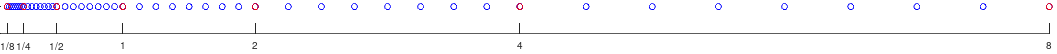
\includegraphics[scale=.4]{escala.png}
\caption{Algunos números positivos de máquina con $b=2$ y $m=4$. Notar que los números son equiespaciados únicamente entre potencias sucesivas de $2$, y que la cantidad de números de máquina en esos rangos se mantiene constante.}
\end{figure}
\begin{tcolorbox}{\bf Distribución de los números de máquina:}
Los números de máquina no se distribuyen de manera uniforme. Describamos dos números de máquina consecutivos  $x_1<x_2$ asumiendo, para simplificar,  que $0<x_1$ y que se escribe:
$$(x_1)_b= 0.b_0b_1b_2...b_{m-1}\, b^{e}.$$
Un momento de reflexión nos dice que el próximo número de máquina (salvo que haya overflow) será
$$(x_2)_b=0.b_0b_1b_2...(b_{m-1}+1)\, b^{e}$$
salvo que $b_{m-1}=b-1$ en cuyo caso
$$(x_2)_b=0.b_0b_1b_2...(b_{m-2}+1)0\, b^{e}$$
salvo que también $b_{m-2}=b-1$ en cuyo caso habrá que repetir el argumento y eventualmente -en caso de que $b_i=b-1$ para todo $0\le i\le m-1$
$$(x_2)_b=0.1b^{e+1}.$$
En cualquier caso observamos que
$$
x_2-x_1=b^{-m}b^e
$$
\emph{no es constante} al variar el exponente $e$, pero sí lo es para cada exponente fijo dado.

\end{tcolorbox}

La consecuencia mas notable de la distribución de los números de máquina es que si $x\in \R$, y existen $x_1<x_2$ números de máquina tales que $x_1\le x\le x_2$ (i.e. $x$ esta dentro de las escalas manejadas por la máquina) entonces
$$
|x-fl_{redond}(x)|\le \frac12 b^{e-m}
$$
$$
|x-fl_{trunc}(x)|\le b^{e-m}
$$
para los casos de redondeo y truncado respectivamente.
\begin{tcolorbox}{\bf Error relativo y precisión de la máquina:}
Nos concentraremos en el caso de redondeo, por lo que asumiremos de aquí en mas que  $fl=fl_{redond}$. Queremos acotar el error relativo al almacenar un número $x\neq 0$.  Observando que
$$b^{e-1}=|0.1\, b^{e}|\le  |x|,$$
resulta
$$
|\frac{x-fl(x)}{x}|\le \frac12 b^{1-m}.
$$
Notar que el error relativo depende \emph{del tamaño de la mantisa}. En el caso de base $b=2$ y $m=52$ mencionado antes resulta:
$$
|\frac{x-fl(x)}{x}|\le  2^{-52}\sim 10^{-16}.
$$
este número, propio de cada máquina, se denomina: precisión de la máquina o épsilon de la máquina y se denota con $\varepsilon$.

En el caso del ejemplo, en terminos simples, dice que nuestra máquina almacena 16 dígitos exactos (en base 10). Naturalemente sería ideal conservar esta precisión a lo largo de las  operaciones que debamos realizar a partir de  $fl(x)$. Eso, como veremos a continuación,  no es posible en general.
\end{tcolorbox}

Como acabamos de ver, en general ocurre que
$x\neq fl(x)$\footnote{Notemos que incluso números muy sencillos como $\frac{1}{10}$ no son de máquina y la introducción de un error de redondeo es inevitable. Evalúe en Python la expresión
$0.1+0.1+0.1!=0.3$, qué obtiene?.}. . Sin embargo podemos garantizar que la diferencia verifica
$$
x-fl(x)=\mu_x x,
$$
con
$$
\frac{|x-fl(x)|}{|x|} =|\mu_x|\le \varepsilon.
$$
Veamos entonces que ocurre con estos errores al efectuar alguna operación
sencilla como por ejemplo sumar. Vamos a distinguir la operación realizada por la máquina con el símbolo $\oplus$.

Pretendemos calcular $x+y$, de modo simplificado la máquina realiza las siguientes operaciones: primero
$$
x\to fl(x) \qquad y\to fl(y)
$$
luego suma $fl(x)+fl(y)$ y finalmente almacena el resultado
$$
fl(x)+fl(y)\to fl(fl(x)+fl(y)).
$$
Cómo se comportará el error resultante?.
Por una lado tenemos:
$$fl(x)=x(1+\mu_x),\qquad  fl(y)=y(1+\mu_y
y),$$ por lo que
$$fl(fl(x)+fl(y))=(fl(x)+fl(y))(1+\mu_z)$$
y en definitiva
$$
x\oplus y =fl(fl(x)+fl(y))=(x(1+\mu_x)+y(1+\mu_y
y))(1+\mu_z).
$$
Vemos entonces que \emph{si $0<x,y$} es posible acotar
$$
|x\oplus y -(x+y)|\le (x+y)2\mu +O(\varepsilon^2)
$$
con $|\mu|\le \varepsilon$. Es decir que hemos de algún modo preservado el tamaño del error relativo\footnote{Cuando los errores se acumulan de forma aditiva, como en este caso, estamos en un buen escenario porque harían falta una enorme cantidad de operaciones para deteriorar el resultado final.}  Como es  bien sabido, eso no es posible si \emph{restamos}
números similares\footnote{Verifique que la cuenta anterior no puede repetirse si los signos de $x$ e $y$ difieren.}.
Un ejemplo elemental es el siguiente: tomemos $b=10$, $m=4$, la precisión es $\varepsilon=\frac{1}{2}10^{-3}=0.0005$. Si $x=125,49$ e $y=125,31$ tenemos respectivamente
$x-y=0.18$
$x\ominus y=0.2$ por lo que el error relativo es
$$
|\frac{x-y-x\ominus y}{x-y}|=\frac{0.02}{0.18}\sim 0.11,
$$
es decir que a pesar de que $\varepsilon \sim 10^{-3}$ el error en la cuenta anterior es del $11\%$. El ejemplo anterior muestra que en una simple operación podemos perder dígitos significativos (de hecho nuestra máquina no ha acertado ningún dígito de la solución). Como regla general deben evitarse restas de números similares\footnote{Ver la guía de ejercicios para mas ejemplos} para evitar la denominada \emph{cancelación catastrófica}.

Es fácil construir ejemplos de números de máquina $0<x<y$ en los cuales no solo $x+y\neq x\oplus y$ sino que, por ejemplo, $x\oplus y=y$. En particular es fácil ver que
\begin{equation}
 \label{eq:epsilonmasuno}
 1 \oplus\varepsilon> 1,
\end{equation}
y
$$
1\oplus\varepsilon/2=1
$$
lo que da una posible definición alternativa del $\epsilon$ como el menor número de máquina con la  propiedad \eqref{eq:epsilonmasuno}.
Otras cuestión que aparece entonces en la aritmética de la máquina es la pérdida de la propiedad asociativa, ya que usando los comentarios previos vemos que por ejemplo
$$
(1\oplus \varepsilon/2)\oplus \varepsilon/2=1\neq 1\oplus (\varepsilon/2+\varepsilon/2).
$$

\section{Estabilidad y Condición}
Hay diversas fuentes de errores computacionales que pueden estropear completamente el resultado de los algoritmos. En este sentido hay dos conceptos que nombraremos tangencialmente ya que no son objeto central de este curso: la \emph{condición} y la \emph{estabilidad}.

De manera muy general, un \emph{problema bien condicionado} es aquél que reacciona benignamente con los errores en los datos. Es decir, que sus soluciones no varían demasiado al no variar demasiado los datos. Por el contrario, si un problema está muy mal condicionado, no lograremos resolverlo con mucha precisión aunque limitemos los errores en los datos (salvo que trabajemos con precisión infinita). La noción de condición es algo \emph{intrínseco del problema} y está mas allá de nuestro algoritmo de resolución.  Por otra parte, cuando los problemas están bien condicionados tenemos esperanza de resolverlos con precisión siempre que nuestro algoritmo no incremente desproporcionadamente los errores inherentes a los datos. En este caso hablaramos de \emph{algoritmos estables} y por el contrario, de  \emph{algoritmos inestables} si no cumplen con este criterio. La estabilidad entonces es algo \emph{intrínseco del algoritmo}.




\begin{tcolorbox}
Es posible dar una expresión precisa para la noción de condición, a través del llamado
\emph{número de condición}. Consideremos el problema de evaluar una función en el valor $x_0$. Si por alguna razón (error de medición o redondeo) modificamos el dato a evaluar $x_0$ en un una cierta magnitud pequeña $h$ entonces el error relativo que cometeremos es (asumiendo que la función es de continuamente diferenciable)
$$
\frac{f(x_0+h)-f(x_0)}{f(x_0)}=
\frac{hf'(\eta)}{f(x_0)},$$
para cierto $\eta$ intermedio entre $x_0$ y $x_0+h$. Esto indica que para $h\sim 0$
$$
\frac{hf'(\eta)}{f(x_0)}\sim
\frac{x_0f'(x_0)}{f(x_0)}\frac{h}{x_0}
$$
el error relativo en los datos $\frac{h}{x_0}$ se magnifica en nuestro problema en un factor
$$
\frac{x_0f'(x_0)}{f(x_0)},
$$
llamado el \emph{número de condición} de evaluar $f$ en $x_0$. Siguiendo un razonamiento similar vemos que para la versión $f:\Rn\to \Rm$ puede definirse el número de condición de este problema de la forma\footnote{Un ejemplo concreto y elemental de mal condicionamiento es, como hemos visto, la resta de números similares: si escribimos
$f:\R^2\to \R$, $f(x,y)=x-y$, se tiene $Df(x_0,y_0)=(1,-1)$, $\|(1,-1)\|_{\infty}=2$, $\|(x_0,y_0)\|_{\infty}=max\{|x_0|,|y_0|\}$, luego $\frac{\|x_0\|\|Df(x_0)\|}{\|f(x_0)\|}\sim \frac{1}{\|x_0-y_0\|}.$

.} $$
\frac{\|x_0\|\|Df(x_0)\|}{\|f(x_0)\|}.
$$
\end{tcolorbox}
Como ejemplo de lo anterior
si queremos evaluar $tg(x)$ en un $x_0<\pi/2$, $x_0\sim \pi/2$ vemos que el número de condición
$$
\frac{x_0}{sen(x_0)cos(x_0)},
$$
cumple que
$$
\lim_{x_0\to \pi/2^-} \frac{x_0}{sen(x_0)cos(x_0)}=+\infty.
$$
En particular si elegimos  $x_0$ tal que $\frac{x_0}{sen(x_0)cos(x_0)}\sim 10^{16}$ no esperamos tener ningún dígito significativo en nuestro cálculo de $tg(x_0)$.


En los años 50, Wilkinson experimentaba con las primeras computadoras y rápidamente comenzó a observar fenomenos de inestabilidades y mal condicionamiento\footnote{En sus propias palabras: ``The cosy relationship that mathematics enjoyed with polynomials suffered a severe setback in the early fifities where electronic computers came into general use. Speaking for myself I regard it as the most traumatic experience in my carrer as a numerical analyst'' \cite{Wil}  }. Una cosa que notó, al probar un algoritmo de aproximación de raices, es que si al polinomio
$$
p(x)=\prod_{i=1}^{20}(x-i)
$$
se le perturba el coeficiente que acompaña a $x^{19}$ (cuyo valor es $210$ ) en $2^{-23}$ las raíces mayores a $7$ sufren considerables modificaciones. En particular las raices  $10,11,\dots 19$
se transforman en 5 pares complejos conjugados. Las $18$ y $19$ en complejos de la forma $19.5\dots\pm 19.5\dots i$, es decir que una perturbación de orden $2^{-23}$ genera variaciones de orden $1$. \footnote{A pesar de esto, se puede probar que las raíces dependen de forma continua respecto de los coeficientes.} Mostrando que el problema de calcular raices está muy mal condicionado.

Ejemplos de algoritmos inestables abundan. La inestabilidad es muy frecuente y se hace notar muy rápidamente porque los resultados obtenidos difieren notoriamente de lo esperado. Los casos mas extremos aparecen en procesos que deben iterarse en los cuales el error se acumula exponencialmente en vez de aditivamente. Sin embargo hay casos muy simples que pueden ejemplificarse.


Mas arriba vimos que restar números similares es un problema mal condicionado y por eso debe evitarse o tratarse con cautela.

Supongamos que queremos evaluar $e^{-12}$. Usando lo explicado mas arriba, podemos ver que se trata de un problema bien condicionado.  Si utilizamos un algoritmo basado en la serie convergente
$$
e^{-x}=1-x+\frac{1}{2!}x^2-\frac{1}{3!}x^3\cdots
$$
para una evaluación directa en $x=-12$ obtenemos, sumando los primeros 50 términos de la serie:
$$
e^{-12}\sim 6.144189436702122\cdot 10^{-6}.$$
Si por otro lado modificamos el algoritmo calculado primero $e^{12}$
sumando los primeros 50 terminos de la serie
$$
e^{x}=1+x+\frac{1}{2!}x^2+\frac{1}{3!}x^3\cdots
$$
y luego invirtiendo $1/e^{12}$ obtenemos
$$e^{-12}\sim 6.144212353328213\cdot 10^{-6}.$$
La pregunta es a priori, cuál de las dos respuestas es mas confiable. Sin duda el segundo método es mas estable. La razón es que en el cómputo de la serie alternada, muchos terminos ``grandes'' deben cancelarse mágicamente para producir el resultado ``pequeño'' $e^{-12}$. Los errores relativos pequeños son proporcionalmente grandes en términos del resultado final. De hecho
$$e^{-12}\sim 6.1442123533282097586823081788055323112239893148882529755...\cdot 10^{-6}$$
es decir que solo obtuvimos $4$ dígitos correctos con nuestro primero algoritmo pero $14$ con el segundo.
El segundo método es mucho mas estable que el primero.


\begin{tcolorbox}{\bf Puede probar los calculos previos con el algoritmo:}\\
\noindent import numpy as np\\
import math     \\
v=np.arange(0,50)\\
resulI=0.0 \\
resulE=0.0 \\
for i in v:\\

\qquad resulI=resulI+1/math.factorial(i)*(-12.0)**i\\

\qquad resulE=resulE+1/math.factorial(i)*(12.0)**i   \\
resulE=1/resulE \\
print(resulInes)\\
print(resulEs)
\end{tcolorbox}
Los problemas que emergen debido a la precisión limitada de las máquinas dan lugar a muchos comportamientos inesperados. Este último ejemplo, debido a Cleve Moler, es particularmente sencillo y sigue las consideraciones del ejemplo previo. Queremos evaluar $p(x)=(x-1)^7$ para posteriormente graficarlo.
En el primer algoritmo usamos la expresión cerrada $(x-1)^7$  y en el segundo método la expresión equivalente
$$
p(x)=x^7-7x^6+21x^5-35x^4+35x^3-21x^2+7x-1.
$$
En la Figura \ref{fig:moler} a la izquierda vemos ambos gráficos perfectamente superpuestos (azul para el segundo método tapado por el rojo del primer método). Para hacer el gráfico usamos los comandos,

\noindent import numpy as np\\
import matplotlib.pyplot as plt\\
x=np.linspace(0,2,200)\\
plt.plot(x,x**7-7*x**6+21*x**5-35*x**4+35*x**3-21*x**2+7*x-1,'b', x,(x-1)**7,'r')\\
plt.show()

\noindent Sin embargo a la derecha vemos el resultado de samplear en una escala mas fina alrededor de la raíz

\noindent x=np.linspace(0.988,1.012,10000)\\
plt.plot(x,x**7-7*x**6+21*x**5-35*x**4+35*x**3-21*x**2+7*x-1,'b', x,(x-1)**7,'r')\\
plt.show()

\begin{figure}
\label{fig:moler}
\includegraphics[scale=0.4]{Moler1}
\includegraphics[scale=0.4]{Moler2}
\caption{Gráficos de $p(x)$}
\end{figure}



Las nociones de condición y estabilidad que hemos comentado de modo superficial son temas transversales a toda el área del análisis  numérico. Como nos restringiremos a cuestiones de álgebra lineal solo hemos pretendido dar una idea somera de sus implicaciones generales. En lo que sigue retomaremos la cuestión de la condición en el ámbito matricial.

\section{Condicion de Matrices}
Sea $\Ab\in \R^{n\times m}$, si no supieramos nada de la sección anterior y quisieramos estudiar la condición de evaluar $\Ab\vb$ (pensado como transformación lineal) notaríamos que podríamos hacerlo bastante en general aprovechando la linealidad.
En efecto, para una perturbación arbitraria $\hb$ de $\vb$ tenemos que el error relativo de evaluar en $\vb$ (asumiendo que $\vb\notin Nu(\Ab)$) puede escribirse
$$
\frac{\|\Ab(\vb+\hb)-\Ab\vb \|}{\|\Ab\vb\|}=\frac{\|\Ab\hb\|}{\|\Ab\vb\|},
$$
y este valor, respecto del error relativo en $\vb$ resulta
$$
\frac{\frac{\|\Ab\hb\|}{\|\Ab\vb\|}}{\frac{\|\vb\|}{\|\hb\|}}=\frac{\|\Ab\hb\|}{\|\hb\|}\frac{\|\vb\|}{\|\Ab\vb\|}\le \|\Ab\|\frac{\|\vb\|}{\|\Ab\vb\|}.
$$
El número que está a la derecha es independiente de $\hb$ y podemos usarlo como representante de la condición de evaluar $\Ab$ en $\vb$ y de hecho vemos que  coincide con la expresión sugerida para la condición en el caso general  (i.e. $
\frac{\|x_0\|\|Df(x_0)\|}{\|f(x_0)\|}
$). Si quisieramos una expresión independiente de $\vb$ que podríamos hacer?. En el caso en que $n=m$ y $\Ab$ sea invertible, podemos llamar $\wb=\Ab\vb$ y el cociente $\frac{\|\vb\|}{\|\Ab\vb\|}$ puede acotarse idependiente de $\vb$
$$
\frac{\|\vb\|}{\|\Ab\vb\|}=
\frac{\|\Ab^{-1}\wb\|}{\|\wb\|}
\le \|\Ab^{-1}\|.$$
En definitiva hallamos un número que mayora a la condición de evaluar en $\vb$ para todo $\vb$ y este es
$$
\|\Ab\|\frac{\|\vb\|}{\|\Ab\vb\|}\le \|\Ab\|\|\Ab^{-1}\|.
$$
Notemos que argumentando con $\Ab^{-1}$, vemos que el mismo número mayora a la condición de evaluar $\Ab^{-1}\wb$. Si bien aún no tenemos aún una clara interpretación del producto $\|\Ab\|\|\Ab^{-1}\|$ vamos a ver que aparece en numerosos escenarios al estudiar la condición de resolver un sistema, por eso lo definimos a continuación.

\begin{defi}{Condición de una matriz}
Dada $\Ab\in \Cnn$ invertible definimos la condición de $\Ab$, $\kappa(\Ab)$, como
$$
\kappa(\Ab)=\|\Ab\|\|\Ab^{-1}\|.
$$
Si $\Ab$ no es invertible definimos que $\kappa(\Ab)=+\infty$.

\end{defi}
Que ocurre si $\Ab\in \C^{n\times m}$? podremos definir algo similar?.  Volveremos sobre este caso mas adelante cuando definamos la \emph{pseudoinversa}.
\begin{remark}
\label{rem:deCondicion}
Observemos que
\begin{enumerate}
 \item La condición de una matriz depende de la norma matricial elegida. Sin embargo, como en dimensión finita todas las normas son equivalentes las condiciones son equivalentes.
\item Para todo $\cero\neq \alpha\in \K$, $\kappa(\alpha\Ab)=\kappa(\Ab)$.
 \item Para toda norma, $1\le \kappa(\Ab)$
\item $\kappa(\Ib)=1$ para toda norma.
\item Para toda $\Qb$ unitaria/ortogonal
$\kappa(\Qb)=1$. (ver item (2) en Proposición \ref{prop:unitarias})
\item $\kappa(\Ab)=\kappa(\Ab^{-1})$
\item Si $\Ab\in \Rnn$ es simétrica, entonces, en norma$-2$, resulta $\kappa(\Ab)=\frac{|\lambda_M|}{|\lambda_m|}$ donde $\lambda_M$ y $\lambda_m$ representan el mayor y el menor autovalor en valor absoluto\footnote{Pues $\|\Ab\|_2=\rho(\Ab)=|\lambda_M|$ y $\|\Ab^{-1}\|_2=\rho(\Ab^{-1})=\frac{1}{|\lambda_m|}$ (ver item (3) de la Observación \ref{rem:sobreautovalores})}.
\end{enumerate}
\end{remark}
Consideremos por un segundo los problemas que pueden aparecer cuando resolvemos un sistema
$$
\Ab\xb=\bb
$$
con $\bb\neq\cero$ y $\Ab$ invertible.
Por un lado tenemos que considerar que tanto $\Ab$ como $\bb$ se almacenaran con errores. En general entonces estaremos resolviendo otro problema
$$
(\Ab+\Delta\Ab)(\xb+\Delta \xb)=
\bb +\Delta \bb.
$$
Asumiendo que procedemos a resolver el problema con aritmética exacta (no hay mas fuentes de error) nos interesa ver el impacto en el error $\Delta \xb$ debido a los errores $\Delta \Ab,\Delta \bb$.

Tenemos, usando que $\Ab\xb=\bb$
$$
\Delta \Ab\xb+\Ab\Delta\xb+\Delta \Ab\Delta \xb=\Delta \bb.
$$
Procediendo \emph{informalmente}, despreciamos el término de ``segundo orden'' $\Delta \Ab\Delta \xb$ y resulta
$$
\Delta \Ab\xb+\Ab\Delta\xb \sim \Delta \bb.
$$
de donde
$$
\Delta \xb\sim \Ab^{-1}\Delta \bb-\Ab^{-1}\Delta \Ab\xb,
$$
y usando que $\|\Ab\|\neq 0$,
$$
\|\Delta \xb\|\lesssim \|\Ab^{-1}\|\|\Delta \bb\|+\|\Ab^{-1}\|\Delta \Ab\|\|\xb\|=\|\Ab^{-1}\|\frac{\|\Delta \bb\|}{\|\bb\|}\|\bb\|+\|\Ab^{-1}\|\frac{\|\Delta \Ab\|}{\|\Ab\|}\|\Ab\|\|\xb\|,
$$
usando que $\|\bb\|\le \|\Ab\|\|\xb\|$ y diviendo por $\|\xb\|\neq \cero$ tenemos
$$\frac{\|\Delta \xb\|}{\|\xb\|}\lesssim \kappa(\Ab)\left(\frac{\|\Delta \bb\|}{\|\bb\|}+ \frac{\|\Delta \Ab\|}{\|\Ab\|}\right).$$
Lo que dice que el error  relativo generado en la solución  se acota en terminos de los errores relativos en los datos por la condición de la matriz.

Observar que en caso de ser $\Delta \Ab=\cero$ (no hay error en la matriz) podemos reemplazar $\lesssim$ con $\le$ y queda
$$\frac{\|\Delta \xb\|}{\|\xb\|}\le \kappa(\Ab)\frac{\|\Delta \bb\|}{\|\bb\|}.$$
De hecho, escribiendo
$\Ab^{-1}\bb=\xb,$ y $\Ab^{-1}(\bb+\Delta\bb)=\xb+\Delta \xb$ se puede argumentar con $\Ab^{-1}$ y por (6) de la Observación \ref{rem:deCondicion}, se ve que
$$\frac{\|\Delta \bb\|}{\|\bb\|}\le \kappa(\Ab)\frac{\|\Delta \xb\|}{\|\xb\|}.$$
Resumiendo
\tcc
$$\frac{1}{\kappa(\Ab)}\frac{\|\Delta \bb\|}{\|\bb\|}\le \frac{\|\Delta \xb\|}{\|\xb\|}\le \kappa(\Ab)\frac{\|\Delta \bb\|}{\|\bb\|}.$$
\etcc
\begin{ej}
 Verifique con ejemplos que las desigualdades previas se alcanzan (Sug.: use matrices diagonales adecuadas).
\end{ej}
Teniendo en cuenta el ejercicio previo, vemos que la cota superior puede alcanzarse en la pŕactica. En particular nos dice de un modo simplificado que podemos perder $log_{10}(\kappa(\Ab))$ dígitos significativos al resolver el sistema\footnote{Por ejemplo, si $\kappa(\Ab)\sim 10^{16}$ no tenemos la garantía de tener ni un dígito correcto en nuestro resultado.}.

El siguiente resultado da una idea cualitativa de $\kappa(\Ab)$ como el recíproco de la distancia relativa de $\Ab$ a las matrices singulares.
\begin{teo}
 $\Ab\in \Rnn$, se tiene,
 \begin{equation}
 \label{eq:minimoasing}
\frac{1}{\kappa(\Ab)}=\inf_{\Bb\,  \mbox{singular}} \frac{\|\Ab-\Bb\|}{\|\Ab\|},
 \end{equation}
 y en donde asumimos $\frac{1}{\kappa(\Ab)}=0$ en caso de que $\Ab$ no sea invertible.
 \end{teo}
 \begin{proof}
  Si $\Ab$ es no invertible el resultado es evidente. Supongamos entonces que $\Ab$ es invertible. Probaremos únicamente que vale  el $\le$  en \eqref{eq:minimoasing}.

  Sea $B\in \Rnn$ una matriz singular cualquiera. Tomemos $\cero\neq \vb\in Ker(\Bb)$, y definamos $\cero\neq\wb=\Ab\vb$. Se tiene
  $$
  0\neq \|\wb\|=\|(\Ab - \Bb)\vb\|\le \|\Ab-\Bb\|\|\Ab^{-1}\wb\|\le \|\Ab-\Bb\|\|\Ab^{-1}\|\|\wb\|,
  $$
  dividiendo por $\|\Ab\|\|\Ab^{-1}\|\|\wb\|\neq 0$ se obtiene
  $$
\frac{1}{\kappa(\Ab)}\le  \frac{\|\Ab-\Bb\|}{\|\Ab\|},
 $$
 y por ser $\Bb$ arbitrario
 $$
\frac{1}{\kappa(\Ab)}\le \inf_{\Bb\,  \mbox{singular}} \frac{\|\Ab-\Bb\|}{\|\Ab\|},
 $$
 \end{proof}
El resultado anterior dice que un número condición grande significa cercanía -relativa- a las matrices singulares. Es importante remarcar que el determinante  no es la herramienta adecuada para medir esa cercanía, pues el ítem (2) de la Observación \ref{rem:deCondicion} dice que el número de condición no cambia por múltiplos de una matriz sin embargo $\det(\alpha\Ab)=\alpha^n\det(\Ab)$ que tiende a cero si $\alpha\to 0$.


falta terminar.....

\section{Proyecciones y Proyectores}
\label{sec:proyectores}
Observemos otra forma equivalente de escribir la proyección ortogonal de $\wb$ sobre el subespacio generado por $\vb$ (ver \eqref{eq:proy_forma1}):
\begin{equation}
 \label{eq:proy_forma2}
 \Pb_{\vb}(\wb)=\frac{\vb}{\|\vb\|_2}\frac{\vb^*}{\|\vb\|_2}\wb,
\end{equation}
que puede verse como una aplicación lineal de matriz  $\frac{\vb\vb^*}{\|\vb\|_2\|\vb\|_2}$.
\tcc
Notar que la matriz $\frac{\vb\vb^*}{\|\vb\|_2\|\vb\|_2}$ , asociada a la proyección $\Pb_{\vb}$, tiene rango $1$.
\etcc
Volvamos un segundo a la ecuación \eqref{eq:escritura_ort}. Si en vez de una base completa solo contamos con un conjunto de vectores ortonormales $\mathcal{C}=\{\vb_1,\cdots,\vb_k\}\subset \Kn$, $k<n$, y llamamos $\mathcal{S}=\langle \vb_1,\cdots,\vb_k\rangle$ al subespacio generado por esos vectores, vemos  que la expresión
\begin{equation}
 \label{eq:proysobreS}
\Pb_{\mathcal{S}}(\wb)=\sum_{1\le i\le k}\Pb_{\vb_i}(\wb).
\end{equation}
verifica
$$
(\wb-\Pb_{\mathcal{S}}(\wb))\perp \vb_j, \qquad \forall 1\le j\le k,
$$
pues
$$
\vb_j*(\wb-\Pb_{\mathcal{S}}(\wb))=\vb_j*\wb -\sum_{1\le i\le k}\vb_j^*\Pb_{\vb_i}(\wb)= \vb_j*\wb-\vb_j*\wb=0.
$$
Luego, por ser ortogonal a todos los generadores de $\mathcal{S}$ lo será a todos lo elementos de $\mathcal{S}$. En otras palabras, teniendo una base ortonormal de $\mathcal{S}$ es muy fácil construir la proyección ortogonal de un elemento $\wb$ sobre  $\mathcal{S}$ usando la expresión \eqref{eq:proysobreS}.
Como además cada $\Pb_{\vb_i}$ admite una representación matricial, lo mismo ocurre con  $\Pb_{\mathcal{S}}$,
$$\Pb_{\mathcal{S}}=
\begin{pmatrix}
&|&&|&&|&\\
&|&&|&&|&\\
\vb_1&|&\vb_2&|&\cdots&|&\vb_k\\
&|&&|&&|&\\
&|&&|&&|&\\
\end{pmatrix}
\begin{pmatrix}
&&&\vb_1^*&&&\\
-&-&-&-&-&-&-\\
&&&\vb_2^*&&&\\
-&-&-&-&-&-&-\\
 &&&\vdots&&& \\
-&-&-&-&-&-&-\\
&&&\vb_k^*&&&
\end{pmatrix}.
$$
\begin{figure}
\includegraphics[scale=0.25]{proyS.png}
%\end{center}
 \label{fig:proyecsobreS}
 \caption{Proyección de $\wb$ sobre el subespacio $\mathcal{S}$.}
%\begin{center}
\end{figure}
Como hemos visto, si queremos entonces obtener la proyección ortogonal de un vector sobre un subespacio $\mathcal{S}$ podemos hacerlo a través de una base ortonormal de $\mathcal{S}$. Sabemos que obtener una familia de generadores de $\mathcal{S}$, $l.i.$ es relativamente sencillo. Sería ideal tener un método para obtener, a partir de esa familia, un sistema de generadores ortonormales. Veamos como hacerlo.

Dada una familia de vectores $\{\vb_1, \vb_2, ...,\vb_n\}$ linealmente independientes. La ortonormalización de Gram-Schmidt
es un algoritmo que produce una sucesión de vectores ortonormales  $\{\qb_1,\qb_2,...,\qb_n\}$ del siguiente modo
El proceso consiste en restarle a cada vector $\vb_i$ sus componentes en los vectores anteriores.

Podemos construir primero una familia ortogonal y luego normalizarla (o normalizarla durante la construcción). Llamemos $\ub_i$ a los ortogonalizados, el método es el siguiente
\begin{itemize}
\item   $\ub_1 = \vb_1$
\item   $\ub_2 = \vb_2 -\Pb_{\ub_1}(\vb_2)$
\item   $\ub_3 = \vb_3 -
\Pb_{\ub_1}(\vb_3)-\Pb_{\ub_2}(\vb_3)$
\item   $\dots$
\item $\ub_k = \vb_k - \sum_{i = 1}^{k-1} \Pb_{\ub_i}(\vb_k)$.
\end{itemize}
Notemos que el algoritmo solo puede detenerse (es decir alcanzar una operación inválida) si y solo si algún $u_k=\cero$ ya que en ese caso, el paso siguiente no puede continuar al no estar definido $\Pb_{\cero}(\wb)$. Pero ocurre si y solo $\vb_k$ es combinación lineal de $\{\vb_1,\vb_2\cdots,\vb_{k-1}\}$\footnote{En efecto, observar que mientras no se detenga el algoritmo $\langle\ub_1,\ub_2,...,\ub_{j}\rangle=\langle\vb_1,\vb_2,..., \vb_{j}\rangle$ para todo $1\le j$.} lo cual contradice el presupuesto de ser $\{\vb_1, \vb_2, ...,\vb_n\}$ linealmente independientes.

En muchos casos  es conveniente utilizar vectores ortonormales  podemos normalizar los vectores obtenidos mediante la fórmula
$$\qb_i = \frac{\ub_i}{\|\ub_i\|}, \quad 1 \le i \le n.$$
También podemos hacerlo a lo largo de la ejecución del algoritmo como se ve debajo.


\begin{center}
\begin{tcolorbox}[width=\linewidth/3]
\begin{center}
{\bf Gramm-Schmidt}
\end{center}


{\bf for} j=1 {\bf to} n

\qquad $\vb_j=\ab_j$

\qquad {\bf for} i=1 to j-1

\qquad\qquad $r_{i,j}=\qb_i^*\ab_j$

\qquad\qquad  $\vb_j=\vb_j-r_{i.j}
\qb_i$


\qquad$r_{j,j}=\|\vb_j\|_2$

\qquad$\qb_{j}=\vb_j/r_{j,j}$

\end{tcolorbox}
\end{center}
Esta familia de vectores verifica,
\begin{itemize}
 \item $\{\qb_1,\qb_2,...,\qb_k\}$ es ortonormal.
 \item $\langle\qb_1,\qb_2,...,\qb_k\rangle=\langle\vb_1,\vb_2,..., \vb_k\rangle$ para todo $1\le k\le n$.
\end{itemize}

Ya hemos hemos notado que las proyecciones ortogonales de vectores sobre subespacios  resultaban aplicaciones lineales.  Vamos a describir las matrices asociadas a esas aplicaciones.
\tccdefi
\begin{defi}
Una matriz $\cero \neq \Pb\in \Knn$ se dice un proyector si
$\Pb^2=\Pb$.
\end{defi}
\etcc

Notar que  dados dos subespacios $S_1,S_2$ tales que $S_1\oplus S_2=\Kn$, siempre es posible construir un proyector $\Pb$ tal que $Im(\Pb)=S_1$ y $Nu(\Pb)=S_2$. En efecto, como los subespacios están en suma directa, para todo $\vb\in \Cn$ existen únicos $\vb_i\in S_i$ tales que
$\vb=\vb_1+\vb_2$. Definiendo $\Pb\vb=\vb_1$ obtenemos el proyector buscado.

Si $\Pb$ es un projector y $\Pb\neq \Ib$ entonces $\Ib-\Pb$ también es un proyector denominado \emph{proyector complementario}.

Un proyector $\Pb$ deja invariante su rango, ya que si $\vb\in Rg(\Pb)$ entonces $\exists \wb$ tal que  $\Pb\wb=\vb$, por lo que
$$
\Pb\vb=\Pb\Pb\wb=\Pb\wb=\vb,
$$
decimos que $\Pb$ proyecta sobre su rango $Rg(\Pb)$.

Notemos que
$$Rg(\Ib-\Pb)=Ker(\Pb),$$
ya que si $\wb\in Rg(\Ib-\Pb)$, es $\wb=\vb-\Pb\vb$ de donde $\Pb\wb=\cero$, i.e. $\wb\in Ker(\Pb)$. Por otro lado, si $\wb\in Ker(\Pb)$,
$Rg(\Ib-\Pb)\ni (\Ib-\Pb)\wb=\wb$. El argumento anterior también implica
$$Rg(\Pb)=Ker(\Ib-\Pb).$$
Por otro lado, se observa trivalmente que  $Ker(\Ib-\Pb)\cap Ker(\Pb)=\{\cero\}$ y entonces
$$Rg(\Pb)\cap Ker(\Pb)=\{\cero\}.$$
Esto dice que
$$
\Kn=Ker(\Pb)\oplus Rg(\Pb).
$$
\tccdefi
\begin{defi}
 Un proyector $\Pb$ se dice \emph{ortogonal} si $Ker(\Pb)\perp Rg(\Pb)$. En otro caso, se dice \emph{oblícuo}.
\end{defi}
\etcc
\tcc
\begin{prop}
\label{prop:ortssiautoadjunto}
Un proyector $\Pb$ es ortogonal sí y solo sí $\Pb=\Pb^*$.
\end{prop}
\etcc
\begin{proof}
 Si $\Pb$ es ortogonal, $\forall, \vb,\wb$
 $$
 0=((\Ib-\Pb)\vb)^*\Pb\wb=\vb^*(\Ib-\Pb)^*\Pb\wb,
 $$
 lo que indica que
 $$
 \cero=(\Ib-\Pb)^*\Pb=\Pb-\Pb^*\Pb,
 $$
 es decir $\Pb=\Pb^*\Pb$ y en particular resulta $\Pb=\Pb^*$.

 Recíprocamente, si $\Pb=\Pb^*$,
 $$
 ((\Ib-\Pb)\vb)^*\Pb\wb=\vb^*(\Ib-\Pb)^*\Pb\wb=\vb^*(\Pb-\Pb^2)\wb=0,
 $$
 $\forall, \vb,\wb$, lo que dice que $\Pb$ es ortogonal.
\end{proof}

\tcc
\begin{teo}
 Sea $\Pb$ un proyector. Son equivalentes:
 \begin{enumerate}
  \item $\Pb$ es ortogonal
  \item $\|\vb\|_2=\|(\Ib-\Pb)\vb\|_2+\|\Pb\vb\|_2$ para todo $\vb$
  \item $\|\Pb\|_2=1$
 \end{enumerate}
\end{teo}
\etcc
\begin{proof}
 $(1)\rightarrow (2)$: para todo $\vb$ escribimos
 $$
 \vb=(\Ib-\Pb)\vb+\Pb\vb,
 $$
 y como por ser proyector $Im(\Ib-\Pb)=Nu(\Pb)\perp Im(\Pb)$, se tiene inmediatamente
 $$\|\vb\|_2=\|(\Ib-\Pb)\vb\|_2+\|\Pb\vb\|_2.$$
$(2)\rightarrow (3)$:
la identidad de $(2)$ dice que
$\|\Pb \vb\|_2\le \| \vb\|_2,$ de donde
$\|\Pb\|_2\le 1$. Como $\Pb$ es proyector,
$\Pb\neq \cero$ y existe $\cero\neq\wb$ tal que $\vb=\Pb\wb\neq\cero$, para ese $\vb$, $\Pb\vb=\vb\neq\cero$ y luego $\|\Pb\|_2\ge 1$, lo dice $\|\Pb\|_2= 1$.

\noindent $(3)\rightarrow (1)$: asumamos que existen $\vb\in Im(\Pb)$ y
$\wb\in Nu(\Pb)$ tales que $\vb^*\wb\neq 0$ y $\|\vb\|=1=\|\wb\|$. Definamos $\ub=\vb-(\wb^*\vb)\wb$, se tiene $\|\Pb\ub\|=\|\Pb\vb\|=\|\vb\|=1$ como $\|\Pb\|=1$ resulta
$$1=\|\Pb\ub\|\le \|\ub\|^2=\|\vb\|^2-
(\wb^*\vb)(\vb^*\wb)-\overline{(\wb^*\vb)}\wb^*\vb+|\wb^*\vb|^2\|\wb\|^2=
$$
$$
1-\overline{(\vb\wb^*)}(\vb^*\wb)-\overline{(\wb^*\vb)}\wb^*\vb+|\wb^*\vb|^2
=1-(\wb^*\vb)^2<1,
$$
absurdos. Luego $Im(\Pb)\perp Nu(\Pb)$ y $\Pb$ es ortogonal.
 \end{proof}

 \begin{tcolorbox}
\begin{rem}
Dada una matriz $\Ab\in\C^{n\times k}$ con columnas \emph{ortonormales}, se tiene que
$\Pb=\Ab\Ab^*\in\C^{n\times n}$ es un proyector ortogonal, ya que al ser $\Ab^*\Ab=\Ib\in \C^{k\times k}$, resulta  $$\Pb^2=\Ab(\Ab^*\Ab)\Ab^*=\Ab\Ab^*=\Pb,$$
i.e. un proyector, además ortogonal por ser
$\Pb^*=\Pb$ (por Proposición \ref{prop:ortssiautoadjunto}).

Llamando $\qb_i$, $1\le i\le k$, a la columna $i$ de $\Ab$, resulta para cada $\vb\in\Cn$, la expresión
$$
\Pb\vb=\Ab\Ab^*\vb=\sum_{1\le i\le k}(\qb_i^*\vb)\qb_i
$$
que clarifica el efecto de multiplicar por $\Pb$.
\end{rem}
\etcc
Vamos a construir una herramienta de  mucha utilidad.  Notemos que para todo $\vb$ de norma uno (de no ser de norma uno dedemos dividir por $\vb^*\vb$ ), podemos definir el proyector ortogonal de rango uno
$$
\Pb_{\vb}=\vb\vb^*,
$$
que proyecta sobre el subespacio generado por $\vb$, y con este su complementario
$$\Pb_{\vb^\perp}=\Ib-\Pb_{\vb},$$
de rango $n-1$ que proyecta sobre el ortogonal a $\vb$.

Como aplicación de estos proyectores podemos reformular Gramm-Schmidt (recordemos que
las columnas de $\Ab$ se donotan con $\ab_i$).
\begin{center}
\begin{tcolorbox}[width=\linewidth/2]
\begin{center}
{\bf Gram-Schmidt Modificado}
 \end{center}

{\bf for} j=1 {\bf to} n

\qquad $\vb_j=\ab_j$

{\bf for} j=1 to n

\qquad $r_{j,j}=\|v_j\|$

\qquad  $\qb_j=\vb_j/r_{j,j}$

\qquad {\bf for} i=j+1 to n

\qquad \qquad$r_{j,i}=\qb^*_j\vb_i$

\qquad \qquad $\vb_{j}=\vb_j - r_{j,i}\qb_j$

\end{tcolorbox}
\end{center}
esta versión modificada,  más estable que la original como veremos con un ejemplo, puede ponerse en términos de proyectores de rango $n-1$. En efecto, habiendo calculado
$\{\vb_1,\cdots,\vb_{j-1}\}$ y $\{\qb_1,\cdots,\qb_{j-1}\}$, el vector $\vb_j$
$$
\vb_j=\Pb_{\qb_{j-1}^{\perp}}\Pb_{\qb_{j-2}^{\perp}}\cdots \Pb_{\qb_{1}^{\perp}}\ab_j.
$$
se obtiene de la aplicación sucesiva de proyectores de este tipo.
\begin{ej}
Hallar la proyección del vector $(1,2)$ sobre la recta generada por el vector $(1,0)$ y la proyección de $(1,0)$ sobre la recta generada por $(1,2)$.

\begin{lstlisting}[language=R]
u = c(1,0)
v = c(1,2)
p = sum(u*v)/sum(u*u) * u
print(p)

q = sum(v*u)/sum(v*v) * v
print(q)
\end{lstlisting}
\end{ej}
\begin{tcolorbox}
\begin{rem}
Gram-Schmidt es ampliamente utilizado en la forma descripta y que funciona generalmente muy bien, sin embargo presenta dificultades numéricas (resulta, como veremos  ser inestable). El costo es TAL
\end{rem}

\end{tcolorbox}
Dada una matriz $\Ab\in \C^{m\times n}$, con columnas $\{\ab_1,\ab_2,\cdots, \ab_n\}$ linealmente independientes, podemos considerar los subespacios anidados generados por sus columnas:
$$
<\ab_1> \subseteq <\ab_1,\ab_2> \subseteq\cdots \subseteq <\ab_1,\ab_2,\cdots, \ab_k>.\footnote{Si las columnas son $l.i.$ las inclusiones son obviamente estrictas, pero no en el caso general.}
$$
En varias aplicaciones es de interés encontrar generadores \emph{ortonormales} de esos subespacios. Esto es, una colección
$\{\qb_1,\qb_2,\cdots ,\qb_k\}$,
tales que $\qb_i^*\qb_j=\delta_i^j$ y
$$
 \langle \ab_1,\ab_2,\cdots, \ab_l\rangle =
 \langle \qb_1,\qb_2,\cdots, \qb_l\rangle
$$
para todo $l$.
Matricialmente, y observando los subespacios anidados, es obvio que esto equivale a hallar una matriz $\Rb\in \Cnn$ triangular
superior
$$
\Rb=
\begin{pmatrix}
 r_{1,1}&r_{1,2}&r_{1,3}&\cdots&r_{1,n}\\
 0&r_{2,2}&r_{2,3}&\cdots&r_{2,n}\\
 0&0&r_{3,3}&\cdot&r_{3,n}\\
 \vdots&\vdots&\vdots&\vdots&\vdots\\
 0&0&0&0&r_{n,n}
\end{pmatrix}
$$
tal que
$$
\begin{pmatrix}
&|&&|&&|&\\
&|&&|&&|&\\
\ab_1&|&\ab_2&|&\cdots&|&\ab_n\\
&|&&|&&|&\\
&|&&|&&|&\\
\end{pmatrix}
=\begin{pmatrix}
&|&&|&&|&\\
&|&&|&&|&\\
\qb_1&|&\qb_2&|&\cdots&|&\qb_n\\
&|&&|&&|&\\
&|&&|&&|&\\
\end{pmatrix}
\begin{pmatrix}
 r_{1,1}&r_{1,2}&r_{1,3}&\cdots&r_{1,n}\\
 0&r_{2,2}&r_{2,3}&\cdots&r_{2,n}\\
 0&0&r_{3,3}&\cdot&r_{3,n}\\
 \vdots&\vdots&\vdots&\vdots&\vdots\\
 0&0&0&0&r_{n,n}
\end{pmatrix},
$$
de donde se observa que tanto los $\qb_i$ (elegidos ortonomales) como los $r_{i,j}$ pueden obtenerse desde las ecuaciones
\begin{eqnarray*}
\ab_1&=&r_{1,1}\qb_1\\
\ab_2&=&r_{1,2}\qb_1+r_{2,2}\qb_2\\
&\vdots&\\
\ab_n&=&r_{1,n}\qb_1+r_{2,n}\qb_2+\cdots r_{n,n}\qb_n\\
\end{eqnarray*}
por ejemplo, a través de Gram-Schmidt. Como hemos mencionado, sin embargo, ese algoritmo no es estable\footnote{Hay una versión modificada utilizando proyectores que veremos mas adelante.} y suelen utilizarse en cambio métodos alternativos. Sin embargo para propósitos teóricos funciona perfectamente.

Notemos que en caso de que $\Qb$ resulte cuadrada ($\Qb\in \C^{n\times n}$), será una matriz unitaria (ortogonal en caso de ser una matriz real). Antes de continuar conviene observar ciertas propiedas de las matrices unitarias.

\section{Matrices Unitarias}

\begin{ej}

Si $\ub = (3, 2, -7)$ y $\vb = (2, 0, 5)$, calcular $\langle \ub, \vb\rangle$ y $\langle \ub + 2\vb, \vb\rangle$.

\begin{lstlisting}[language=R]
u = c(3, 2, -7)
v = c(2, 0, 5)
sum(u*v)
sum((u+2*v) * v)
\end{lstlisting}

Si $\langle \ub, \vb \rangle$ = 7 y $\langle \vb, \wb\rangle = -2$ y $\|\vb\| = 4$, calcular:
\begin{enumerate}
\item $\langle 3\ub, 4\vb\rangle$
\item $\langle 2\vb, \vb + \ub - 5\wb\rangle$
\end{enumerate}
\end{ej}



\subsection{Bases ortogonales - Proceso de Gram-Schmidt}

Dado un conjunto de vectores $\{\xb_1, \dots, \xb_s\}$ (linealmente independientes) el proceso de Gram-Schmidt permite obtener un nuevo conjunto ortogonal de vectores $\{\ub_1, \dots, \ub_s\}$ tal que $\langle \xb_1, \dots, \xb_t\rangle = \langle \ub_1, \dots, \ub_t\rangle$ para todo $1 \le t \le s$.


\begin{ej}
Aplicar el proceso de Gram-Schmidt a los vectores $\xb_1 = (1, 0, 0)$, $\xb_2 = (2, 3, -1)$ y $\xb_3=(0, 7, -2)$.

\begin{lstlisting}[language=R]
x1 = c(1, 0, 0)
x2 = c(2, 3, -1)
x3 = c(0, 7, 2)

# Hacemos la cuenta para u2:
u1 = x1
u2 = x2 - sum(u1*x2)/sum(u1 * u1) * u1
print(u1)
print(u2)
print(u2 / sqrt(sum(u2^2)))

A = cbind(x1, x2, x3)
gS = gramSchmidt(A)
print(gS)
#gS$Q %*% t(gS$Q)
\end{lstlisting}
\end{ej}


Dado un subespacio vectorial $V = \langle \vb_1, \dots, \vb_s \rangle \subset \R^n$, decimos que un conjunto de vectores $\{\wb_1, \dots, \wb_t\}$ es una base ortonormal de $V$ si

\begin{itemize}
\item $\|\wb_i\| = 1$ para todo $1 \le i \le t$.
\item $\langle \wb_i, \wb_j \rangle = 0$ para $i \neq j$.
\end{itemize}

Dada una base cualquiera $\B$ de un espacio vectorial, podemos obtener una base ortonormal aplicando el proceso de Gram-Schmidt.

\subsection{Matrices ortogonales}

Recordemos que una matriz $\Ab \in \mathbb{R}^{n \times n}$ es ortogonal si $\Ab \Ab^T = I_n$. Si $f_1, \dots, f_n$ son las filas de $\Ab$, $\Ab$ es ortogonal si
$$
\langle f_i , f_j\rangle =
\begin{cases}
1 & \text{ si } i = j \\
0 & \text{ si } i \ne j
\end{cases}.
$$
Es decir, todas las filas tienen norma-2 igual a 1 y son perpendiculares entre sí.





\chapter{Sistemas y Factorización de Matrices}

Comenzaremos asumiendo que trabajaremos con matrices cuadradas, i.e.  $\Ab\in \R^{n\times n}$ (o mas en general
$\C^{n\times n}$ ya que la mayoría de las consideranciones se aplican a los complejos).

Los vectores $\vb\in \Cn$ los identificamos con matrices columna de $n\times 1$ de donde tiene sentido $\Ab\vb$.

Factorizar siginifica descomponer una expresión en factores de algún modo mas simples o que nos otorguen algún beneficio teórico o práctico. La factorización
LU consiste en escribir una matriz invertible $\Ab$ como producto de dos factores: uno triangular inferior $\Lb$ y otro triangular superior $\Ub$. Un beneficio inmediato de esta factorización es que para  resolver un sistema
$$
\Ab\xb=\bb,
$$
basta resolver
$$
\Lb\yb=\bb,
$$
$$
\Ub\xb=\yb,
$$
y cada sistema triangular puede resolverse por sustitución (regresiva o progresiva) en $\sim n^2$ operaciones
\begin{ej}Resolución sistemas triangulares: dar un algoritmo para resolverlo en orden $n^2$
\end{ej}
\begin{ej}Resolución sistemas tridiagonales: dar un algoritmo para resolverlo en orden $n$:
{\bf Motivar con ecuaciones diferenciales-}
\end{ej}

\section{Descomposición $\Lb\Ub=\Ab$}

La factorización $LU$ es un subproducto del método de eliminación de Gauss.
Dada la matriz
$$
\Ab= \begin{pmatrix}
a_{1,1}& a_{1,2} & \cdots & a_{1,n} \\
a_{2,1} & a_{2,2} & \cdots & a_{2,n} \\
\vdots  & \vdots  & \ddots & \vdots  \\
a_{n,1} & a_{n,2} & \cdots & a_{n,n}
\end{pmatrix}
$$
y suponiendo que $a_{1,1}$, denominado \emph{pivot}, es no nulo es posible operar
sobre las filas de $\Ab$ para generar ceros debajo del elemento
$a_{1,1}$. Esto se hace fila a fila multiplicando la fila 1 de $\Ab$ por $-\frac{a_{i,1}}{a_{1,1}}$ (lo cual es
posible ya que hemos asumido  $a_{1,1}\neq 0$) y sumando ese resultado a
la fila $i$. En términos matriciales, eso
equivale a multiplicar a izquierda la matriz $\Ab$ por el
multiplicador $\Mb_1$
$$
\Mb_1 =
\begin{pmatrix}
1 & 0 & \cdots & 0 \\
-\frac{a_{2,1}}{a_{1,1}} & 1 & \cdots & 0 \\
\vdots  & \vdots  & \ddots & \vdots  \\
-\frac{a_{n,1}}{a_{1,1}} & 0 & \cdots & 1
\end{pmatrix} $$
El efecto neto del producto resulta
$$
\Mb_1\Ab= \begin{pmatrix}
a_{1,1}& a_{1,2} & a_{1,3} &\cdots & a_{1,n} \\
0 & a^{(1)}_{2,2} & a^{(1)}_{2,3} &\cdots & a^{(1)}_{2,n} \\
0 & a^{(1)}_{3,2} & a^{(1)}_{3,3} & \cdots & a^{(1)}_{3,n} \\

\vdots  & \vdots  & \ddots & \vdots  \\
0 & a^{(1)}_{n,2}& a^{(1)}_{n,3} & \cdots & a^{(1)}_{n,n}
\end{pmatrix}
$$
donde se destaca con un superíndice $(1)$ una nueva matriz
$\Ab^{(1)}\in \R^{(n-1)\times (n-1)} $
$$
\Ab^{(1)}=
 \begin{pmatrix}
 a^{(1)}_{2,2} & \cdots & a^{(1)}_{2,n} \\
\vdots  & \vdots  & \ddots &   \\
a^{(1)}_{n,2} & \cdots & a^{(1)}_{n,n}
\end{pmatrix}
$$
que en caso de tener el pivot $a^{(1)}_{2,2}\neq 0$ admite un nuevo paso en la iteración tomando
$$
\Mb_2 =
\begin{pmatrix}
1 & 0 & \cdots & 0 & 0 \\
0 & 1& \cdots & 0 & 0 \\
0 & -\frac{a_{3,2}^{(1)}}{a^{(1)}_{2,2}} & 1 & \cdots & 0 \\
\vdots  & \vdots  & \vdots & \vdots  \\
0&-\frac{a_{n,2}^{(1)}}{a^{(1)}_{2,2}} & 0 & \cdots & 1
\end{pmatrix} $$
de donde
$$
\Mb_2\Mb_1\Ab= \begin{pmatrix}
a_{1,1}& a_{1,2} & a_{1,3} &\cdots & a_{1,n} \\
0 & a^{(1)}_{2,2} & a^{(1)}_{2,3} &\cdots & a^{(1)}_{2,n} \\
0 & 0 & a^{(2)}_{3,3} & \cdots & a^{(2)}_{3,n} \\

\vdots  & \vdots  & \ddots & \vdots  \\
0 & 0& a^{(2)}_{n,3} & \cdots & a^{(2)}_{n,n}
\end{pmatrix}
=\begin{pmatrix}
a_{1,1}& a_{1,2} & a_{1,3} &\cdots & a_{1,n} \\
0 & a^{(1)}_{2,2} & a^{(1)}_{2,3} &\cdots & a^{(1)}_{2,n} \\
0 & 0 & &  &  \\
\vdots  & \vdots &  & \Ab^{(2)} &   \\
0 & 0&  &
\end{pmatrix},
$$
con $\Ab^{(2)}\in \R^{(n-2)\times (n-2)}$.
Este procedimiento, dado que cada $\Mb_i$ es triangular, se denomina  \emph{triangulación por matrices triangulares}. Si algoritmo no se detiene, es decir que cada elemento pivot $a_{k+1,k+1}^{(k)}\neq 0$, para todo $1\le k\le n-1$, se obtiene una matriz triangular superior $\Ub$ invertible
$$
\Mb_{n-1}\Mb_{n-2}\cdots \Mb_{1}\Ab=\Ub=
\begin{pmatrix}
a_{1,1}& a_{1,2} & a_{1,3} & a_{1,4}&\cdots & a_{1,n} \\
0 & a^{(1)}_{2,2} & a^{(1)}_{2,3} & a^{(1)}_{2,4} &\cdots & a^{(1)}_{2,n} \\
0 &0 & a^{(2)}_{3,3} & a^{(2)}_{3,4}  &\cdots & a^{(2)}_{3,n} \\
%|0 & 0 & 0 &  & & \\
\vdots  & \vdots & \vdots  & \vdots  & \vdots  & \vdots   \\
0 & 0& 0 & 0& 0& a^{(n-1)}_{n,n}
\end{pmatrix}
$$
Observemos que la productoria
$$
\Mb_{n-1}\cdots\Mb_2\Mb_1=\Mb,
$$
es una matriz triangular inferior, dado que es producto de matrices triangulares inferiores. La inversa de $\Mb$, es por lo tanto triangular inferior. La llamaremos $\Lb=\Mb^{-1}$ y por ende
$$
\Ab=\Lb\Ub.
$$
El problema que aparece inmediatamente es que no hemos obtenido $\Lb$ constructivamente (en el sentido de que aún falta invertir $\Mb$). Sin embargo, un hecho notable facilita ese trabajo.

Observemos que cada $\Mb_i$ tiene la forma
\begin{equation}
 \label{eq:formaMi}
\Mb_i=\Ib-\zb_i\eb_i^T,
\end{equation}
donde
$\eb_i$ representa el $i-$ésimo canónico y
$\zb_i$ es de la forma
$$
\zb_i=
\begin{pmatrix}
 0\\
 \vdots\\
 0\\
 z_{i+1}^{(i)}\\
 \vdots \\
 z_n^{(i)}
\end{pmatrix},
$$
con $z_j^{(i)}=\frac{a^{(i-1)}_{j,i}}{a^{(i-1)}_{i,i}}$, $i+1\le j\le n$.

\begin{tcolorbox}[colback=black!15!white,colframe=black!75!black]
\begin{lema}\label{lema:inversamultiplicador}
 Sea $\ub,\vb\in \Rn$, tales que $\vb^T\ub\neq 1$ entonces $\Ib-\ub\vb^T$ es invertible y además
 $$(\Ib-\ub\vb^T)^{-1}=\Ib+\frac{\ub\vb^T}{1-\vb^T\ub}.$$
\end{lema}
\end{tcolorbox}
\begin{proof}
 $$(\Ib-\ub\vb^T)(\Ib+\frac{\ub\vb^T}{1-\vb^T\ub})=\Ib+\ub\vb^T(\frac{1}{1-\vb^T\ub}-1)-\frac{\ub\vb^T\ub\vb^T}{1-\vb^T\ub}=\Ib. $$
\end{proof}
Considerando el lema anterior y observando que en  \eqref{eq:formaMi} se tiene
$\eb_i^T\zb_i=0$, resulta \footnote{Es decir que el costo de invertir $\Mb_i$ es casi nulo (apenas un cambio de signos debajo de la diagonal).}
$$
\Mb_i^{-1}=\Ib+\zb_i\eb_i^T,
$$
de donde
$$
\Lb=\Mb_1^{-1}\Mb_2^{-1}\cdots \Mb_{(n-1)}^{-1}=(\Ib+\zb_1\eb_1^T)(\Ib+\zb_2\eb_2^T)\cdots (\Ib+\zb_{n-1}\eb_{n-1}^T).
$$
Ademas de la sencillez en el cómputo de $\Mb_i^{-1}$ hay otro hecho ``afortunado'' que permite expresar $\Lb$ sin cálculos adicionales. Como $\eb_i^T\zb_k=0$ no solo para $k=i$ sino para todo $i\le k\le n$,  se puede desarrollar la expresión para $\Lb$ y obtener
$$
\Lb=\Ib+\sum_{i=1}^{n-1}\zb_i\eb_i^T,
$$
o dicho de otra forma,
$$
\Lb=
\begin{pmatrix}
1 & 0 & \cdots & 0 & 0\\
\frac{a_{2,1}}{a_{1,1}} & 1 & \cdots & 0 & 0 \\
\frac{a_{3,1}}{a_{1,1}} & \frac{a_{3,2}^{(1)}}{a^{(1)}_{2,2}}
\vdots  & \vdots  & \ddots & \vdots  \\
\vdots  & \vdots  & \ddots &1&  \vdots  \\
\frac{a_{n,1}}{a_{1,1}} &  \frac{a_{n,2}^{(1)}}{a^{(1)}_{2,2}} & \cdots & \frac{a_{n,n-1}^{(n-1)}}{a^{(n-1)}_{n-1,n-1}}& 1
\end{pmatrix},
$$
i.e., basta con almacenar los multiplicadores en sus respectivos lugares cambiando los signos.




Un supuesto básico para que la descomposición LU pueda llevarse a cabo
es que todos los pivots sean no nulos.
Eso no puede garantizarse bajo la única hipótesis de que $det(\Ab)\neq 0$ como se ve en tomando por ejemplo
$$
\Ab=
\begin{pmatrix}
 0&1\\
 1&0
\end{pmatrix}
$$

Sin embargo puede garantizarse si se requiere que todos lo menores de la matriz $\Ab$,
sean invertibles.

\begin{tcolorbox}
[colback=black!15!white,colframe=black!75!black]
\begin{prop}\label{prop:menorenonulos}
 Sea $\Ab\in \Rnn$, entonces existe factorización LU de $\Ab$ con $\Lb,\Ub$ \emph{invertibles} sí y solo sí
 para todo  $1\le k\le n$,  $det(\Ab(1:k,1:k))\neq 0$.
\end{prop}

\end{tcolorbox}
 \begin{proof}
  hacer...
 \end{proof}

Para ver otro criterio necesitamos una definición.
\tccdefi
\begin{defi}
  \label{defi:deDD}
  Una matriz $\Ab\in \Rnn, \Cnn$ se dice \emph{diagonal dominante} (\emph{estrictamente diagonal dominante}) y se denota DD (EDD) si y solo si para todo $i$,
 $1\le i\le n$
 $$
 \sum_{1\le j \le n, j\neq i}|a_{i,j}|\le (<) |a_{i,i}|.
 $$

 \end{defi}
\end{tcolorbox}
Y la siguiente proposición (que puede refinarse en algunos casos como veremos mas adelante).
\tcc
\begin{prop}
 Sea $\Ab\in \Rnn, \Cnn$ EDD entonces $\Ab$ es invertible.
\end{prop}
\etcc
\begin{proof}
 Supongamos que no. Existe entonces
 ${\bf 0}\neq \vb\in\Cn$ tal que
 $\Ab\vb=\cero$. Sea $i$, $1\le i\le n$ tal que $0\neq |v_i|=\|\vb\|_\infty$, entonces
 $$
 \sum_{j=1}^na_{i,j}v_j=0,
 $$
 de donde
 $$
 |a_{i,i}|\le \sum_{j=1, j\neq i}^n|a_{i,j}|\frac{|v_j|}{|v_i|}\le
 \sum_{j=1, j\neq i}^n|a_{i,j}|,
 $$
 lo que contradice la EDD.
\end{proof}






\begin{tcolorbox}
[colback=black!15!white,colframe=black!75!black] \begin{prop}
  Si $\Ab$ es EDD entonces, trabajando con aritmética exacta, el proceso de eliminación de Gauss no produce pivots nulos.
 \end{prop}
\end{tcolorbox}
\begin{proof}
 hacer...
\end{proof}

\begin{tcolorbox}
\begin{rem}
 Las matrices DD no son una artificio teórico, aparecen frecuentemente en la práctica. En particular en la discretización de ecuaciones diferenciales, como veremos en algún ejemplo mas adelante.

 Citaría el caso de las tridigonales clásicas y las de dos variables...
 observaría que no es EDD y agregaría algo de la teoría del libro de Ortega.
\end{rem}
\etcc

Aún en el caso en que no aparezcan pivots nulos, el algoritmo de eliminación no delvoverá en general los verdaderos factores $\Lb$ y $\Ub$, sino una aproximación de ellos. Mas explícitamente podemos enunciar el siguiente teorema.
\begin{tcolorbox}
[colback=black!15!white,colframe=black!75!black]
\begin{teo}\label{teo:errorLU}
 Sea $\Ab\in \Rnn$, y $\tilde\Ab=fl(\Ab)$, si el algoritmo LU no produce pivots nulos,la factorización LU producida por la máquina verifica
 $$
 \tilde\Lb\tilde \Ub=\tilde \Ab + \Hb
 $$
donde $|\Hb|\lesssim 2(n-1)\mu(|\tilde \Ab|+|\tilde \Lb||\tilde \Ub|)
+\mathcal{O}(\mu^2).
$
\end{teo}

\end{tcolorbox}
\begin{proof}
 hacer ... no es larga.
\end{proof}


\begin{tcolorbox}
\begin{rem}
 El Teorema \ref{teo:errorLU}, sugiere controlar el tamaño de los factores
$\tilde\Lb,\tilde\Ub$. En efecto, si el producto
$|\tilde \Lb||\tilde \Ub|$ es muy grande no tendremos control (al menos teórico) sobre el error. El \emph{pivoteo parcial} permite garantizar al menos el control $|\Lb|\le 1$ a una costo razonable. Si bien, esto no necesariamente implica que $|\tilde \Lb||\tilde \Ub|$ sea pequeño, resulta suficiente en la mayoría de los casos prácticos (ver sin embargo la Observación \ref{obs:malgauss}).

\end{rem}

\end{tcolorbox}


\begin{ej}
 Muestre el el número de operaciones necesarias para realizar la factorización LU es $\mathcal{O} (\frac{2n^3}{3})$
\end{ej}

El número de elementos de una matriz de $n\times n$ es obviamente $n^2$. El número mínimo de operaciones que un método de resolución puede efectuar debe ser de orden mayor o igual a $n^2$. Todos los métodos directos clásicos son de orden cúbico. Esto presenta problemas para matrices muy grandes ya que en las aplicaciones es posible tener mas de $10^6$ incógnitas.

Otro problema importante es el \emph{rellenado} que produce el algoritmo. Esto es, aunque $\Ab$ sea \emph{rala} -cosa que afortunadamente ocurre en muchas aplicaciones, como en ecuaciones diferenciales- los factores $\Lb,\Ub$ pueden no serlo.

\begin{ej}
 Cuanta memoria ocuparía una matriz
 de $10^6\times 10^6$ llena?.
\end{ej}



\section{Descomposición $\Lb\Ub=\Pb\Ab$ (pivoteo parcial)}
Una matriz de permutaciones $\Pb\in \Rnn$
es una matriz identidad con las filas permutadas. Observemos las siguientes propiedades de las permutaciones.
\begin{itemize}
 \item Dada $\Ab\in \Rnn$, $\Pb\Ab$ coincide con $\Ab$ pero con las filas permutadas y $\Ab\Pb$ coincide con $\Ab$ pero con las columnas permutadas.
 \item Dada $\xb\in \Rn$, $\Pb\xb$ coincide con $\xb$ pero con los elementos permutados.
 \item $det(\Pb)=\pm 1$
 \item $\Pb^{-1}=\Pb^T$
 \item Si $\Pb_1$ y $\Pb_2$ son permutaciones entonces $\Pb=\Pb_1\Pb_2$ también lo es.
\end{itemize}
\begin{tcolorbox}
Esto es para poner mas adelante---
 \begin{rem}
 \begin{enumerate}
  \item Las matrices de Markov (también llamadas estocásticas) verifican que $0\le a_{i,j}\le 1$
  y $\sum_{j=1}^na_{i,j}=1$. Es decir que cada fila puede interpretarse como una distribución discreta de probabilidad (mas adelante retomaremos este tema).
  \item Una matriz es bi-estocástica si tanto $\Ab$ como $\Ab^T$ son de Markov. Puede probarse que toda matriz de este tipo es combinación convexa de matrices de permutaciones
  (Teorema de Brikhoff-Von Neumann).
 \end{enumerate}
 \end{rem}
\end{tcolorbox}


Si durante la eliminación de Gauss hallamos un pivot nulo, podemos intercambiar filas para continuar con el algoritmo (siempre que haya algún elemento no nulo con el cual proseguir). Mas aún, aunque el correspondiente pivot sea no nulo, podemos,  casi al mismo costo, tomar el pivot mas grande (en valor absoluto) para  garantizar que $|\tilde\Lb|\le 1$.  Esa operación la podemos representar matricialmente multiplicando por una adecuada permutación.

El procedimiento sería el siguiente: tomemos el elemento con mayor valor absoluto en la primera columna de $\Ab$. Digamos que este es $a_{k,1}$ (si $det(\Ab)\neq 0$ se tiene que $a_{k,1}\neq 0$). Permutemos la fila $k$ con la fila $1$, lo cual se hace con una matriz $\Pb_1$. Es decir
$$
\Pb_1\Ab=
\begin{pmatrix}
 a_{k,1}&a_{k,2}&\cdots &a_{k,n}\\
 a_{2,1}&a_{2,2}&\cdots &a_{2,n}\\
  \vdots&\vdots&\vdots&\vdots\\
 a_{1,1}&a_{1,2}&\cdots &a_{1,n}\\
 \vdots&\vdots&\vdots&\vdots \\
 a_{n,1}&a_{n,2}&\cdots &a_{n,n}
\end{pmatrix},
$$
a partir de aquí construimos el multiplicador, $\Mb_1$ de modo tal que
$$
\Mb_1\Pb_1\Ab=
\begin{pmatrix}
 a_{k,1}&a_{k,2}&\cdots &a_{k,n}\\
 0&&&\\
  \vdots&&\Ab^{(1)}&\\
 0&&&\\

\end{pmatrix}.
$$
Llegado a este punto, repetimos el procedimiento con la primer columna de $\Ab^{(1)}$ que eventualmente requerirá otra matriz $\Pb_2$ antes de la construcción del nuevo multiplicador $\Mb_2$. En definitiva,
\begin{equation}
 \label{eq:factoresPLU}
\Mb_{n-1}\Pb_{n-1}\cdots \Mb_{1}\Pb_{1}\Ab=\Ub,
 \end{equation}


se obtiene una nueva matriz triangular superior $\Ub$, y donde
$\Mb_i=\Ib-\zb_i\eb_i^T$ con
$$
\zb_i=
\begin{pmatrix}
 0\\
 \vdots\\
 0\\
 z_{i+1}^{(i)}\\
 \vdots \\
 z_n^{(i)}
\end{pmatrix},
$$


$|\zb_i|\le 1$ (i.e. los multplicadores sin menores o iguales a 1 en valor absoluto).
El problema ahora es que en la forma \eqref{eq:factoresPLU}  no parece verse el modo de reconstruir los factores $\Lb$ y $\Pb$ de forma sencilla. Sin embargo otro hecho inesperadamente favorable resuelve esta cuestión. Notemos que por el orden de las iteraciones en el paso $k$ solo permutaremos en busca del mayor pivot (en caso de ser necesario) filas desde la $k$ a la $n$ porque las filas previas ya han sido procesadas. Eso indica que
$\eb_j^T\Pb_k=\eb^T_j$ para todo $j<k$. En particular, si bien \emph{no es cierto} que $\Pb_k$
conmuta con $\Mb_j$ sí es cierto,
\emph{para todo $j<k$}, que
$$
\Pb_k\Mb_j=\Pb_k
(\Ib-\zb_{j}\eb_{j}^T)=
(\Ib-\Pb_k\zb_{j}\eb_{j}^T)\Pb_k=
\tilde\Mb_j \Pb_k,
$$
es decir que podemos pasar la permutación a la derecha permutando adecuadamente los multiplicadores de la matriz $\Mb_j$. Lo importante es que esta nueva matriz, denotada con $\tilde \Mb_j$ tiene la misma estructura que $\Mb_j$. Así que volviendo a  \eqref{eq:factoresPLU} tenemos
$$
\Mb_{n-1}\Pb_{n-1}\cdots \Mb_{1}\Pb_{1}\Ab= \tilde \Mb_{n-1}\cdots \tilde \Mb_{1} \Pb_{n-1}\cdots \Pb_{1}\Ab=\Ub.
$$
Argumentando como en el caso son pivoteo (usando que la estructura de las $\tilde \Mb_i$ es igual a la de las de las $\Mb_i$) y llamando
$\Pb=\Pb_{n-1}\cdots \Pb_{1}$ se llega a
$$
\Pb\Ab=\Lb\Ub.
$$

\begin{tcolorbox}
[colback=black!15!white,colframe=black!75!black] \begin{prop}
  Trabajando con aritmética exacta se tiene que si $det(\Ab)\neq 0$ el algoritmo de pivoteo parcial no tiene pivots nulos.
 \end{prop}
\end{tcolorbox}

\begin{tcolorbox}
[colback=black!15!white,colframe=black!75!black] \begin{rem}
\label{obs:malgauss}
El proceso de pivoteo parcial garaniza que $|\Lb|\le 1$ pero no
se un tiene control demasiado beningno sobre el tamaño de
$|\Ub|$, como se ve en este ejemplo
$$
\begin{pmatrix}
 1&0&0&\cdots&0&1\\
 -1&1&0&\cdots&0&1\\
 -1&0&1&0&\cdots&1 \\
 \vdots &\vdots&\vdots& \ddots&&\vdots\\
 -1&0&0&0&\cdots&1
\end{pmatrix},
$$
puede verse que $\|\Ub\|_\infty \ge 2^n\|\Ab\|_\infty$.
Este ejemplo sin embargo parece ser singular en el sentido de que en los casos genéricos el crecimiento de $|\Ub|$ estaría controlado por $\sqrt{n}$ \cite{TB} \footnote{Al presente no parece haber una demostración de esto aunque Trefethen ofrece un premio de 200 dólares por una. Buscar el SIAM news donde esta esto.} Esta particularidad parece (junto con el hecho de que su costo es la mitad que el de la factorización $QR$ que veremos mas adelante) haber mantenido el algoritmo de eliminación como uno de los más populares entre los métodos directos.
 \end{rem}
\end{tcolorbox}

Controlar el tamaño del ambos factores $\Lb$ y $\Ub$ es posible.
La idea se denomina \emph{pivoteo completo}, esto implica hacer permutaciones de filas y de columnas para tomar siempre el mayor pivot posible. Así en el paso inicial se busca el elemento $a_{k,l}$ con máximo valor absoluto y se permutan la fila y columna 1 con la fila y columna $k$ y $l$ respectivamente.  En términos matriciales eso requiere de dos matrices de permutaciones $\Pb_1,\tilde \Pb_1$ antes de aplicar el paso de eliminación. Es decir
$$
\Mb_1\Pb_1\Ab\tilde\Pb_1=
\begin{pmatrix}
 *&*&\cdots &*\\
 0&&&\\
  \vdots&&\Ab^{(1)}&\\
 0&&&\\

\end{pmatrix}.
$$
Repitiendo el procedimiento se obtiene $\Ub$
$$
\Mb_{n-1}\Pb_{n-1}\cdots \Mb_1\Pb_1\Ab\tilde\Pb_1\cdots \tilde\Pb_{n-1}=\Ub,
$$
y argumetando como antes se obtienen ahora dos matrices de permutaciones $\Pb,\tilde\Pb$ tales que
$$
\Pb\Ab\tilde\Pb=\Lb\Ub.
$$
El pivoteo completo no se lleva a cabo en general debido a su alto costo.  (poner el costo... suponiendo que las comparaciones valen por operaciones tradicionales). Ya que hay otros métodos estables mas económicos. Wilkinson probó lo siguiente
\tcc
\begin{teo}
 En aritmética exacta, para el algoritmo de pivoteo completo se tiene
 $$
 \|\Ub\|_{\infty}\le \sqrt{n}(2.3^{1/2}.4^{1/3}\cdots n^{1/(n-1)})^{1/2}\|\Ab\|_\infty
 $$
\end{teo}
\etcc
\begin{ej}
 Estimar el crecimiento del factor
 $\sqrt{n}(2.3^{1/2}.4^{1/3}\cdots n^{1/(n-1)})^{1/2}$.
\end{ej}

\begin{itemize}
 \item falta hablar de unicidad de LU
\end{itemize}

\section{Descomposición $\Lb \Db\Lb^*$ : Cholesky}


En muchos casos es posible explotar la estructura de las matrices a la hora de resolver sistemas. Dicho sea esto a la hora de ahorrar computos o mejorar la estabilidad de los algoritmos.


\begin{prop}
\label{prop:defposesinvert}
Si $\Ab$ es definida positiva entonces es invertible y también lo son todos sus menores.
\end{prop}
\begin{proof}
 En efecto, de no ser invertible, existiría $\cero\neq\vb$ tal que
 $\Ab\vb=\cero$ lo que contradice la definida positividad ya que para ese $\vb$ se tendría $\vb^*\Ab\vb=0$.

 Respecto de los menores el resultado se sigue del anterior. En efecto, sea $k$ fijo, $1\le k\le n$ y tomemos
 vectores $\vb\in \C^n$ de la forma
 $(\tilde \vb,0,\cdots,0)$ con $\tilde \vb \in \C^k$ arbitrario. Resulta
 $$
 0<\vb^*\Ab\vb=\tilde\vb^*\Ab(1:k,1:k)\tilde \vb,
 $$
 y de ahí la definida positividad de $\Ab(1:k,1:k)$ y por ende su invertibilidad.
\end{proof}


Si $\Ab$ es definida positiva  admite una descomposición $\Ab=\Lb\Ub$ (gracias a las Proposiciones \ref{prop:defposesinvert} y \ref{prop:menorenonulos}) y
podemos escribir  $\Ub=\Db\tilde \Lb^*$, con $\tilde \Lb$ triangular inferior con $1$ en la diagonal y $\Db$ una matriz diagonal. De ahí resulta
$$
\Ab=\Lb\Db\tilde{ \Lb}^*=\tilde \Lb\Db^*\Lb^*,
$$
entonces
$$
\Db(\Lb^{-1}\tilde{ \Lb})^* = \Lb^{-1}\tilde \Lb\Db^*,
$$
y como el lado izquierdo de esta ecuación es triangular superior y el derecho triangular inferior deberán ser ambos diagonales. Luego, debe serlo también $\Lb^{-1}\tilde \Lb$. Por  construcción, $\tilde\Lb_{i,i}=1=\Lb_{i,i}$, para todo $1\le i\le n$ . Debido a la primera igualdad se tiene en particular que
$\Lb^{-1}_{i,i}=1$. De aquí resulta
$\Lb^{-1}\tilde \Lb=\Ib$, es decir
$\Lb=\tilde \Lb$ y además $\Db=\Db^*$.
En particular se obtiene la factorización
$$
\Ab=\Lb\Db\Lb^*.
$$
Como además $\Ab$ es definida positiva, entonces $\Db>0$, pues para todo $\vb\neq 0$
$$
0<\vb^*\Ab\vb=\vb^*\Lb\Db\Lb^*\vb=
(\Lb^*\vb)^*\Db\Lb^*\vb,
$$
de donde, llamando $\wb=\Lb^*\vb$ y usando que $\Lb$ (y por ende $\Lb^*$) es invertible, resulta la definida positividad de $\Db$, lo que en este caso, por ser diagonal, equivale a $\Db>0$. Esto nos garantiza la existencia de la factorización de Cholesky:
$$
\Ab=\Lb\Db^{\frac{1}{2}}\Db^{\frac{1}{2}}\Lb^*=\Cb\Cb^*,
$$
donde $\Cb$ es triangular inferior con elementos diagonales positivos. La construcción de $\Cb$ puede hacerse desde la factorización LU, sin embargo
ese modo mas costoso y menos estable que el algoritmo que describiremos debajo. Antes, sin embargo, veamos cómo sería la base de un algoritmo (garantizando que pueda ejecutarse sin interrupciones).

Asociemos el algoritmo con una función $chol()$\footnote{En Python $np.linalg.cholesky()$ en Matlab $chol()$.}. Es decir $chol(\Ab)$ devuelve el factor $\Cb$.

Ya que $\Ab=\Cb\Cb^*$, con $\Cb$ triangular inferior $c_{i,i}>0$, (de hecho, ya probamos la existencia de esta factorización). Intentaremos ``despejar'' $\Cb$.

Escribimos
$$
\Cb=
\begin{pmatrix}
 c_{1,1}&|&\cero \\
 -&-&-\\
 \Cb(2:n,1)&|&\Cb(2:n,2:n)
\end{pmatrix}
$$
donde $\Cb(2:n,2:n)$ tiene las mismas características que $\Cb$. Sabiendo que
\begin{eqnarray}
\label{eq:desc_de_A_:w
Chol}
\begin{pmatrix}
 a_{1,1}&|&\Ab(2:n,1)^* \\
 -&-&-\\
 \Ab(2:n,1)&|&\Ab(2:n,2:n)
\end{pmatrix}&= \\ \nonumber
\begin{pmatrix}
 c_{1,1}&|&\cero \\
 -&-&-\\
 \Cb(2:n,1)&|&\Cb(2:n,2:n)
\end{pmatrix}
&
\begin{pmatrix}
 c_{1,1}&|&\Cb(2:n,1)^* \\
 -&-&-\\
 \cero&|&\Cb(2:n,2:n)^*
\end{pmatrix}
\end{eqnarray}
se tiene, respectivamente, que
$$
\mbox{\bf Paso 1}  \qquad c_{1,1}^2=a_{1,1} \qquad \to \qquad c_{1,1}:=\sqrt{a_{1,1}},
$$

$$
\mbox{\bf Paso 2} \ \  \Ab(2:n,1)=c_{1,1}\Cb(2:n,1)\qquad\to\qquad \Cb(2:n,1):=\Ab(2:n,1)/c_{1,1},
$$

lo cual nos permitió ``despejar'' las incógnitas $\Cb(1:n,1)$, puesto que
$a_{1,1}>0$ por hipótesis, lo que permite elegir $c_{1,1}>0$. Ahora consideramos
$$
\mbox{\bf Paso 3} \ \ \Ab(2:n,2:n)=\Cb(1:n,1)\Cb(1:n,1)^*+\Cb(2:n,2:n)\Cb(2:n,2:n)^* \to $$
$$\Cb(2:n,2:n):= chol(\Ab(2:n,2:n)-\Cb(1:n,1)\Cb(1:n,1)^*),
$$
de donde el problema de resolver
$chol(\Ab(1:n,1:n))$ para una matriz de $n\times n$  se redujo
a resolver $chol(\Ab(2:n,2:n)-\Cb(2:n,1)\Cb(2:n,1)^*)$ para una matriz de tamaño $(n-1)\times (n-1)$, lo que inductivamente (siempre que la nueva matriz sea definida positiva) nos lleva al problema trivial de factorizar un número real positivo (matriz de $1\times 1$ definida positiva) como el cuadrado de otro positivo. Veamos entonces la siguiente
\tcc
\begin{prop}
 Si $\Ab$ es SDP entonces $\Ab(2:n,2:n)-\Cb(2:n,1)\Cb(2:n,1)^*$, donde
 $\Cb=(2:n,1)=\Ab(2:n,1)/\sqrt{a_{1,1}}$, es DP.
\end{prop}
\etcc
\begin{proof}
Claramente $\Ab(2:n,2:n)-\Cb(2:n,1)\Cb(2:n,1)^*$ es Hermitiana (o simétrica, en el caso real). Por otro lado, y por hipótesis, para todo $\cero\neq \ub=(u_1,\vb)\in \Cn$ se tiene
 $$
 0<\ub^*\Ab\ub=
 \begin{pmatrix}
  u_1\\
  -\\
  \vb
 \end{pmatrix}^*
\begin{pmatrix}
 a_{1,1}&|&\Ab(2:n,1)^* \\
 -&-&-\\
 \Ab(2:n,1)&|&\Ab(2:n,2:n)
\end{pmatrix}
 \begin{pmatrix}
  u_1\\
  -\\
  \vb
 \end{pmatrix}=
 $$
 $$
 |u_1|^2 a_{1,1}+u_1^{*}\Ab(2:n,1)^{*}\vb +u_1\vb^*\Ab(2:n,1)+\vb^*\Ab(2:n,2:n)\vb.
 $$
 Elijamos $u_1=-\frac{\Ab(2:n,1)^*\vb}{a_{1,1}}$ y resulta para todo $\vb\neq \cero$,
 $$
 0<\vb^*\left( \Ab(2:n,2:n)-\Cb(2:n,1)\Cb(2:n,1)^*\right)\vb,
 $$
 lo que completa la demostración.
\end{proof}
En forma de algoritmo, Cholesky puede
escribirse del siguiente modo,

{\bf for} j= 1:n

\qquad $a_{j,j}:=\sqrt{a_{j,j}}$

\qquad {\bf for} i=j+1:n

\qquad \qquad $a_{i,j}:=a_{i,j}/a_{j,j}$


\qquad {\bf for} k=j+1:n

\qquad\qquad\qquad  {\bf for} i=k:n

\qquad\qquad\qquad    $a_{i,k}:=a_{i,k}-a_{i,j}a_{k,j}$

en donde se utliliza solo la información de la parte triangular  inferior de $\Ab$ (la parte superior es redundante) y en donde, además, se almacenan los datos de la matriz $\Cb$.


\begin{itemize}

 \item dar  la complejidad $\frac{1}{3}n^3$
 \item Comentar porque es estable-
\end{itemize}



\section{Ortogonalidad}

\begin{tcolorbox}
Como hemos mencionado, el método de eliminación se basa en triangulación por matrices triangulares (los multiplicadores).
El crecimiento de los  multiplicadores y de la matriz triangular superior resultante podría ser problemático.  Por esa razón lo ideal sería realizar operaciones con matrices de norma controlada (idealmente de norma 1). Esos algoritmos son posibles y se basan en ideas de ortogonalidad.
\end{tcolorbox}


Dada una matriz $\Ab\in \C^{m\times n}$, con columnas $\{\ab_1,\ab_2,\cdots, \ab_n\}$ linealmente independientes, podemos considerar los subespacios anidados generados por sus columnas:
$$
<\ab_1> \subseteq <\ab_1,\ab_2> \subseteq\cdots \subseteq <\ab_1,\ab_2,\cdots, \ab_k>.\footnote{Si las columnas son $l.i.$ las inclusiones son obviamente estrictas, pero no en el caso general.}
$$
En varias aplicaciones es de interés encontrar generadores \emph{ortonormales} de esos subespacios. Esto es, una colección
$\{\qb_1,\qb_2,\cdots ,\qb_k\}$,
tales que $\qb_i^*\qb_j=\delta_i^j$ y
$$
 \langle \ab_1,\ab_2,\cdots, \ab_l\rangle =
 \langle \qb_1,\qb_2,\cdots, \qb_l\rangle
$$
para todo $l$.
Matricialmente, y observando los subespacios anidados, es obvio que esto equivale a hallar una matriz $\Rb\in \Cnn$ triangular
superior
$$
\Rb=
\begin{pmatrix}
 r_{1,1}&r_{1,2}&r_{1,3}&\cdots&r_{1,n}\\
 0&r_{2,2}&r_{2,3}&\cdots&r_{2,n}\\
 0&0&r_{3,3}&\cdot&r_{3,n}\\
 \vdots&\vdots&\vdots&\vdots&\vdots\\
 0&0&0&0&r_{n,n}
\end{pmatrix}
$$
tal que
$$
\begin{pmatrix}
&|&&|&&|&\\
&|&&|&&|&\\
\ab_1&|&\ab_2&|&\cdots&|&\ab_n\\
&|&&|&&|&\\
&|&&|&&|&\\
\end{pmatrix}
=\begin{pmatrix}
&|&&|&&|&\\
&|&&|&&|&\\
\qb_1&|&\qb_2&|&\cdots&|&\qb_n\\
&|&&|&&|&\\
&|&&|&&|&\\
\end{pmatrix}
\begin{pmatrix}
 r_{1,1}&r_{1,2}&r_{1,3}&\cdots&r_{1,n}\\
 0&r_{2,2}&r_{2,3}&\cdots&r_{2,n}\\
 0&0&r_{3,3}&\cdot&r_{3,n}\\
 \vdots&\vdots&\vdots&\vdots&\vdots\\
 0&0&0&0&r_{n,n}
\end{pmatrix},
$$
de donde se observa que tanto los $\qb_i$ (elegidos ortonomales) como los $r_{i,j}$ pueden obtenerse desde las ecuaciones
\begin{eqnarray*}
\ab_1&=&r_{1,1}\qb_1\\
\ab_2&=&r_{1,2}\qb_1+r_{2,2}\qb_2\\
&\vdots&\\
\ab_n&=&r_{1,n}\qb_1+r_{2,n}\qb_2+\cdots r_{n,n}\qb_n\\
\end{eqnarray*}
por ejemplo, a través de Gram-Schmidt. Como hemos mencionado, sin embargo, ese algoritmo no es estable\footnote{Hay una versión modificada utilizando proyectores que veremos mas adelante.} y suelen utilizarse en cambio métodos alternativos. Sin embargo para propósitos teóricos funciona perfectamente.

Notemos que en caso de que $\Qb$ resulte cuadrada ($\Qb\in \C^{n\times n}$), será una matriz unitaria (ortogonal en caso de ser una matriz real). Antes de continuar conviene observar ciertas propiedas de las matrices unitarias.

\section{Matrices Unitarias}
De todas la matrices, las unitarias poseen propiedades especiales que las hacen muy favorables para su uso en los algoritmos.
\tcc
\begin{prop}
 \label{prop:unitarias}
 Sea $\Ab\in \C^{m\times n}$, $\Qb\in \Cnn$, $\Qb$ unitaria, resulta
 \begin{enumerate}
  \item $\forall \vb\in \Cn$
  $\|\Qb\vb\|_{2}=\|\vb\|_2$
  \item $\|\Qb\|_{2}=1$
  \item $\|\Qb\Ab\|_2=\|\Ab\|_2$
  \item $\|\Qb\Ab\|_F=\|\Ab\|_F$

 \end{enumerate}
\gabo{falta la propiedad de que es invariante para la norma de los valores singulares: sirve para SVD, darlo en su momento}
\end{prop}
\etcc
\begin{proof} Para $(1)$ escribimos
 $$
 \|\Qb\vb\|_{2}^2=(\Qb\vb)^*(\Qb\vb)=\|\vb\|_2^2,
 $$
 ya que $\Qb^*\Qb=\Ib$.

 El ítem $(2)$ sale inmediatamente de $(1)$.

 Para $(3)$, notemos que por $(1)$ se tiene
 $$\|\Qb\Ab \|_{2}=sup_{\vb, \|\vb\|=1}
 \|\Qb\Ab \vb\|_{2}=sup_{\vb, \|\vb\|=1}\|\Ab\vb\|_2=\|\Ab\|_2.
 $$
 Finalmente, para $(4)$ escribimos
 $$
 \|\Qb\Ab\|_F^2=tr((\Qb\Ab)^*(\Qb\Ab))=tr((\Ab^*\Ab)=\|\Ab\|_F^2.
 $$

\end{proof}

Vemos, gracias a la proposición anterior, que para toda $\Ab\in \C^{n\times m}$ y $\Qb\in \Cnn$ el producto $\Qb\Ab$ se realiza en la máquina de modo estable. Ya que
$$
fl(\Ab)=\Ab + \Eb \,\, \mbox{y }\,  fl(\Qb)=\Qb + \Fb,
$$
con
$$
\|\Eb\|_2\le C(n)\varepsilon
\|\Ab\|_2
$$
$$
\|\Fb\|_2\le C(n)\varepsilon,$$
donde hemos usado que $\|\Qb\|_2=1$.
Por lo tanto
$$
fl(\Qb)fl(\Ab)=(\Qb + \Fb)(\Ab + \Eb)=\Qb\Ab+\Fb\Ab+\Qb\Eb+\Fb\Eb,
$$
y usando la Proposición \ref{prop:unitarias} resulta
$$
fl(\Qb)fl(\Ab)=\Qb\Ab+\Gb,
$$
donde
$$
\|\Gb\|_2\le \epsilon C(n)\|\Ab\|_2+\mathcal{O}(\epsilon^2),
$$
de donde el resultado computado por la máquina verifica

$$
fl(fl(\Qb)fl(\Ab))=fl(\Qb\Ab+\Gb)=\Qb\Ab+\tilde\Gb,
$$
con
$$
\|\tilde \Gb\|_2\le \epsilon C(n)\|\Ab\|_2+\mathcal{O}(\epsilon^2),
$$
que establece la estabilidad de multplicar por $\Qb$.


\section{Factorización QR}
\tcc
\begin{teo}
Dada $\Ab\in \C^{m\times n}$ es posible escribirla como producto de dos factores $\tilde \Qb\in \C^{m\times n}$ y $\Rb\in \C^{n\times n}$.
 \end{teo}
\etcc

\begin{proof}
 Si $\Ab$ tiene sus columnas $l.i.$
 la construcción se obtiene del algoritmo de Gram-Schmidt. En efecto, el algoritmo solo fallará cuando algún $\vb_j$ sea cero y no se pueda dividir por $r_{j,j}$. De hecho eso implicaría que en ese paso $\ab_j\in \langle\qb_1,\cdots\qb_{j-1}\rangle=\langle\ab_1,\cdots\ab_{j-1}\rangle$ lo que contradice el hecho de que las columnas de $\Ab$ sean $l.i.$.

 En el caso en el que las columnas de $\Ab$ no sean $l.i.$, el algoritmo fallará del modo descripto. De ser así, elegimos $\qb_j$, $l.i.$ con
 $\{\qb_1,\cdots\qb_{j-1}\}$ y continuamos con el procedimiento las veces que sea necesario.

 En ambos casos se obtiene
 $$
 \Ab=\Qb\Rb.
 $$

 Esta factorización suele llamarse \emph{reducida} debido a que la matriz
 $\Qb$ no es cuadrada. Sin embargo, en el caso  $m\ge n$ siempre será posible
 completar $\{\qb_1,\cdots\qb_n\}$ a una base de $\C^m$ y agregar ceros adecuadamente en la matriz $\Rb$ para mantener la igualdad $\Ab=\Qb\Rb$ del modo siguiente
 $$
 \stackrel{
 \begin{pmatrix}
  &&&&\\
  &&&&\\
  &&&&\\
  &&\Ab&&\\
  &&&&\\
  &&&&\\
  &&&&\\
  &&&&
 \end{pmatrix}=}{m\times n}
  \stackrel{\begin{pmatrix}
  &&&&\\
  &&&&\\
  &&&&\\
  &&\Qb&&\\
  &&&&\\
  &&&&\\
  &&&&\\
  &&&&
  \end{pmatrix}}{m \times m }\stackrel{ \begin{pmatrix}
  r_{1,1}&r_{1,2}&r_{1,3}&\cdots&r_{1,n}\\
 0&r_{2,2}&r_{2,3}&\cdots&r_{2,n}\\
 0&0&r_{3,3}&\cdot&r_{3,n}\\
 \vdots&\vdots&\vdots&\vdots&\vdots\\
 0&0&0&0&r_{n,n}\\
 0&0&0&0&0\\
 \vdots&\vdots&\vdots&\vdots&\vdots\\
 0&0&0&0&0
 \end{pmatrix}}{\underbrace{m\times n}},
 $$
que se denomina factorización QR \emph{completa}.
 \end{proof}
 Consideremos la factorización reducida. Podemos multiplicar una columna arbitraria, digamos la columna $j$,  de $\Qb$ por un complejo $z$ de la forma $e^{i\theta}\neq 1$ y la fila $j$ por $z^{-1}=e^{-i\theta}$ obteniendo una nueva factorización QR reducida, el resultado siguiente dice que salvo esa modificación, la factorización es única.
\tcc
\begin{teo}
Dada $\Ab\in \C^{m\times n}$ con $m\ge n$ y rango máximo existe una única factorización reducida con la propiedad de que $\R \ni r_{i,i}>0$.
 \end{teo}
\etcc


\begin{proof}
 llll
\end{proof}


\begin{itemize}
 \item Poner complejidad de usar Gramm-Schmidt
 \item Householder y mencionar Givens
 \item Resolución de sistemas por QR
\end{itemize}



Otra aplicación notable de los proyectores se ve en la siguiente sección.

\section{QR vía reflectores de Householder.}

En la factorización $LU=A$ se triangula $A$ por medio de \emph{matrices triangulares}. Hemos visto, sin embargo,  que resulta costoso controlar el tamaño de ambos factores en términos del tamaño de la matriz $A$ (se debe utilizar pivoteo completo). Por otro lado, hemos visto también que el algoritmo clásico de Gramm-Schmidt puede verse como un proceso de ortogonalización por matrices triangulares, algo que podemos denominar \emph{ortogonalización triangular}.

Con la idea de buscar un método mas estable, nos preguntamos si es posible triangular con matrices ortogonales (unitarias) u
ortogonalizar con matrices ortogonales (unitarias).


Consideremos un vector  $\vb\in \Cm$, y veamos si podemos construir una matriz $\Hbb_{\vb}\in \Cmm$ \emph{unitaria} tal que $\Hbb_{\vb}\vb=\alpha\eb_1\in \Cm$ (la notación $\Hb$ es por Householder). Es decir, un múltiplo del canónico $\eb_1$.
Si esto es posible en general, veremos que entonces también es posible  triangular una matriz multiplicando por matrices ortogonales.

La primera observación importante es que por ser $\Hbb_{\vb}$ unitaria, la propiedad (1) de la Proposición \ref{prop:unitarias} dice que en caso de existir tal matriz debe ser $|\alpha|=\|\vb\|_2$, ya que $\|\vb\|_2=\|\Hbb_{\vb}\vb\|_2=|\alpha|\|\eb_1\|_2$.  Habiendo dicho eso, concentremos primero nuesta intuición en el caso real es decir $\vb\in \R^n$ y veamos un modo  posible  de construir $\Hbb_{\vb}$ con  una \emph{reflexión} a través del hiperplano ortogonal a $\wb=\|\vb\|\eb_1-\vb$  \gabo{(dibujito)}.

Consideremos primero el proyector $\Pb_{\wb}=\frac{\wb\wb^T}{\wb^T\wb}$, y su complementario $\Pb_{\wb^\perp}=\Ib-\Pb_{\wb}$. Si seguimos mas allá del hiperplano $\wb^\perp$ podemos \emph{reflejar} el vector $\vb$ sobre el eje generado por $\eb_1$. Mas  específicamente
$$
\Hbb_{\vb}=\Ib-2\Pb_{\wb},
$$
produce la reflexión deseada.

En efecto,
$$\Hbb_{\vb}\vb=\vb-2\Pb_{\wb}\vb=\vb - 2\frac{(\|\vb\|\eb_1-\vb)(\|\vb\|\eb_1-\vb)^T}{(\|\vb\|\eb_1-\vb)^T(\|\vb\|\eb_1-\vb)}\vb=$$
$$= \vb-2\frac{(\|\vb\|\eb_1-\vb)(\|\vb\|v_1-\|\vb\|^2)}{2\|\vb\|^2-2v_1\|\vb\|}
=\vb+\|\vb\|\eb_1-\vb=\|\vb\|\eb_1.$$
Observemos que en efecto $\Hbb_{\vb}$ resulta ortogonal ya que  por un lado es simétrica por serlo $\Pb_{\wb}$, y entonces

$$
\Hbb_{\vb}\Hbb_{\vb}^T=\Hbb_{\vb}^2=
(\Ib-2\Pb_{\wb})(\Ib-2\Pb_{\wb})=
\Ib-4\Pb_{\wb}+4\Pb_{\wb}=\Ib,
$$
donde hemos usado en la anteúltima identidad el hecho de que $\Pb_{\wb}$ es un proyector.

Notemos que de haber utilizado $\wb=-\|\vb\|\eb_1-\vb$, se hubiera obtenido otra matriz ortogonal
$\tHb_{\vb}$ con la propiedad
$$
\tHb_{\vb}\vb=-\|\vb\|\eb_1.
$$
Si bien ambas cumplen con el propósito teórico de llevar $\vb$ al eje $x_1$, computacionalmente conviene elegir aquella que resulte  ser mas estable. Para ello queremos garantizar que $\vb$ no sea similar al vector que elijamos (de las dos opciones $\pm\|\vb\|\eb_1$) para construir la reflexión  (con la idea de evitar la resta de vectores  similares en el cómputo de $\wb$).  Esto claramente puede sistematizarse tomando \footnote{Convendremos, para evitar ambiguedades,  en tomar  $sg(v_1)=1$ si $v_1=0$.}
$$
\wb=sg(v_1)\|\vb\|\eb_1-\vb.
$$

El procedimiento se extiende análogamente  a $\Cm$. Ahí escribimos nuevamente $v_1=sg(v_1)v_1$, donde $sg(v_1)$ es el complejo de módulo uno dado por $sg(v_1)=e^{i\theta}$ y
con la misma construcción para $\wb$, tenemos que
$$
\Hbb\vb=\vb-2\frac{\wb\wb^*}{\wb^*\wb}\vb \in \langle \eb_1 \rangle,
$$
en efecto
$$\Hbb\vb=\vb - 2\frac{(\|\vb\|e^{i\theta}\eb_1-\vb)(\|\vb\|e^{i\theta}\eb_1-\vb)^*}{(\|\vb\|e^{i\theta}\eb_1-\vb)^*(\|\vb\|e^{i\theta}\eb_1-\vb)}\vb=
$$
$$
 =\vb-2\frac{(\|\vb\|e^{i\theta}\eb_1-\vb)(\|\vb\||v_1|-\|\vb\|^2)}{2\|\vb\|^2-2|v_1|\|\vb\|}=\|\vb\|e^{i\theta}\eb_1.
$$
En este punto notamos que si
$\Ab\in \Cmm$ es invertible (o mas en general, $\Ab\in \Cmn$ con columnas $l.i$) siempre puede construirse $\Hb_1\in \Cmm$  de modo tal que
$$
\Hb_1\Ab=
\begin{pmatrix}
 \star&*&\cdots &*\\
 0&&&\\
  \vdots&&\Ab^{(1)}&\\
 0&&&\\
\end{pmatrix},
$$
en  donde $\star$ es no nulo y de valor absoluto la norma de la primer columna de $\Ab$ y donde resulta tener $\Ab^{(1)}$ columnas $l.i.$ (ya que $\Hbb_1$ es invertible y $\Ab$ tiene columnas $l.i.$) por lo cual podemos iterar el procedimiento en una dimensión menor y tomar
$\Hbb^{(1)}\in \C^{(m-1)\times (m-1)}$ unitaria de modo tal que al multiplicar por
$$
\Hbb_2=\begin{pmatrix}
 1&0&\cdots &0\\
 0&&&\\
  \vdots&&\Hbb^{(1)}&\\
 0&&&\\
\end{pmatrix},
$$
 se obtenga
$$
\Hbb_2\Hbb_1\Ab=
\begin{pmatrix}
 \star&*&\cdots &*\\
 0&\star&\cdots&*\\
 0&0&\cdots&*\\
  \vdots&\vdots&\Ab^{(2)}&\\
 0&0&&\\
\end{pmatrix},
$$
con
$\Ab^{(2)}\in \C^{(m-2)\times (m-2)}$ de columnas $l.i$.
Obviamente el procedimiento puede continuarse sin interrupciones hasta tener (suponiendo $m>n$, de ser $m=n$  la matriz $\Rb$ resultante es cuadrada)
$$
\Hbb_{n-1}\cdots \Hbb_2\Hbb_1\Ab=
\begin{pmatrix}
 \star&*&\cdots &*\\
 0&\star&\cdots&*\\
 0&0&\cdots&*\\
 0&0&\cdots&\star\\
 0&0&&0\\
  \vdots&\vdots&\vdots&\vdots\\
 0&0&&0
\end{pmatrix}=\Rb,
$$
es decir que tenemos otra vez
$$
\Ab=\Qb\Rb
$$
donde, $\Qb$ es
\begin{equation}
 \label{ec:Q}
\Qb=(\Hbb_{n-1}\cdots \Hbb_2\Hbb_1)^{-1}=\Hbb_{1}\cdots \Hbb_{n-2}\Hbb_{n-1},
\end{equation}

ya que cada $\Hbb_j$ es unitaria y Hermitiana.

El algoritmo puede escribirse

\begin{tcolorbox}[width=\linewidth*4/5]
\begin{center}
{\bf QR vía Householder}

\end{center}

{\bf for} j=1 {\bf to} n

\qquad $\vb_j=\ab_j(j:m)$

\qquad $\wb_j=sg(\vb(1))\|\vb\|_2\eb_1+\vb$

\qquad  $\wb_j=\wb_j/\|\wb_j \|_2$

\qquad  $\Ab(j:m,j:n)= \Ab(j:m,j:n)-2\wb_j(\wb_j^*\Ab(j:m,j:n))$
\end{tcolorbox}
Notemos que la matriz
$\Hbb=\Hbb_{n-1}\cdots \Hbb_2\Hbb_1$ no se construye explícitamente durante el algoritmo sino que sólo se multiplica por las $\Hbb_i$
(de hecho solo por la parte significativa de las  $\Hbb_i$ que tienen dimensión
$(m-i)\times (m-i)$).

En caso de querer resolver $\Ab x=\bb$, con $\Ab\in \Cnn$ puede hacerse sin llegar a la factorización, aplicando $\Hbb$ a $\bb$, es decir, como
$$
\Hbb\Ab=\Rb,
$$
basta resolver
$$
\Rb \xb= \Hbb \bb,
$$
que tiene solución única (si $\Ab$ es invertible). Algorítmicamente, $\Hbb \bb,$ se obtiene durante la ejecución como se ve debajo

\begin{tcolorbox}[width=\linewidth*4/5]
\begin{center}
{\bf QR vía Householder y \textcolor{red}{cómputo de $\tilde \Qb\bb$}}
\end{center}

{\bf for} j=1 {\bf to} n

\qquad $\vb_j=\ab_j(j:m)$

\qquad $\wb_j=sg(\vb(1))\|\vb\|_2\eb_1+\vb$

\qquad  $\wb_j=\wb_j/\|\wb_j \|_2$

\qquad  $\Ab(j:m,j:n)= \Ab(j:m,j:n)-2\wb_j(\wb_j^*\Ab(j:m,j:n))$

\qquad \textcolor{red}{$\bb(j:m)=\bb(j,:m)-2\wb_j(\wb_j^*\bb(j:m))$}
\end{tcolorbox}
una vez mas, sin construir $\Hbb$ explícitamente.

Más aún, incluso en el caso rectangular $m>n$, teniendo en cuenta el cálculo simultáneo de los productos
$$
\Hbb_{n-1}\cdots \Hbb_2\Hbb_1\Ab \qquad \Hbb_{n-1}\cdots \Hbb_2\Hbb_1\bb,
$$
a lo largo del algoritmo y usando el hecho de que la matrices unitarias preservan la norma 2 (citar proposición) resulta
$$
\|\Ab\xb-\bb\|_2=\|\Hbb_{n-1}\cdots \Hbb_2\Hbb_1(\Ab\xb-\bb)\|_2=
\|
   \Rb\xb-\Hbb\bb
\|_2,
$$
que dice que aún en el caso rectangular y aunque no podamos garantizar la existencia de un $\xb$ tal que $\Ab\xb=\bb$ podríamos intentar minimizar la diferencia\footnote{Esta es la propuesta de  \emph{mínimos cuadrados}, tema que trataremos con detalle mas adelante.} $\Ab\xb-\bb$ y el algoritmo previo provee los instrumentos para la resolución de ese problema, ya que la identidad
$$
\|\Ab\xb-\bb\|_2=  \| \Rb\xb-\Hbb\bb\|,
$$
dice que el mínimo puede hallarse calculando el $\xb$ que verifica
$\Rb(1:n,1:n)\xb=\Hbb\bb(1:n).$

Notemos que almacenando $\wb_j$ durante la  ejecución (que equivale a conocer los $\Hb_j$) podemos multiplicar un vector cualquiera $\zb$ por $\Qb$, sin necesidad de contruir $\Qb$ explícitamente.
En efecto, gracias a \eqref{ec:Q}, vemos que $\Qb\zb$ puede calcularse haciendo los productos en orden inverso,

\begin{tcolorbox}[width=\linewidth*4/5]
\begin{center}
{\bf \textcolor{red}{Cómputo de $\Qb\zb$}}
\end{center}

{\bf for} j=n {\bf to} 1

\qquad \textcolor{red}{$\zb(j:m)=\zb(j,:m)-2\wb_j(\wb_j^*\zb(j:m))$}
\end{tcolorbox}
Observemos que de ser necesario el cálculo explícito de $\Qb$, pude hacerse con el algoritmo anterior multiplicando
$\Qb\eb_i$ con $1\le i\le  m$.
\section{QR vía rotaciones de Givens}
Ademas de las simetrías hay otras transformaciones unitarias, estas últimas se basan en rotaciones. Dado $\cero\neq
\begin{pmatrix}
a\\
b
\end{pmatrix}
\in \C^2$ queremos, como en el caso de Householder, construir una matriz unitaria $\Gb\in \C^{2\times 2}$ ($\Gb$ por Givens) tal que
$$
\Gb\begin{pmatrix}
a\\
b
\end{pmatrix}
=
\begin{pmatrix}
\star\\
0
\end{pmatrix}
$$
con $\star=\left\|
\begin{pmatrix}
a\\
b
\end{pmatrix}\right\|.
$
Una vez mas comencemos mirando el caso real, i.e. $(a,b)\in \R^{2}$ y recordemos la forma de las matrices de rotaciones de ángulo $\beta$,
$$
\begin{pmatrix}
 cos(\beta)&-sen(\beta)\\
 sen(\beta)&cos(\beta)
\end{pmatrix},
$$
i.e. dado un vector $\begin{pmatrix}
cos(\theta)\\
sen(\theta)
\end{pmatrix},$ el producto
$$\begin{pmatrix}
 cos(\beta)&-sen(\beta)\\
 sen(\beta)&cos(\beta)
\end{pmatrix}\begin{pmatrix}
cos(\theta)\\
sen(\theta)
\end{pmatrix}=\begin{pmatrix}
cos(\theta+\beta)\\
sen(\theta+\beta)
\end{pmatrix},$$
produce la rotación mencionada. En particular, tomando $\beta=-\theta$ vemos que la rotación transforma el vector $\begin{pmatrix}
cos(\theta)\\
sen(\theta)
\end{pmatrix}$ en el canónico $\eb_1=\begin{pmatrix}
1\\
0
\end{pmatrix}$.
En general, dado $(a,b)\in \R^{2}$, escribimos
$$
(a,b)= \sqrt{a^2+b^2}(cos(\theta),sen(\theta))=
\left\|
\begin{pmatrix}
a\\
b
\end{pmatrix}\right\|(cos(\theta),sen(\theta)),
$$
donde
$$
cos(\theta)=\frac{a}{\sqrt{a^2+b^2}}\qquad
sen(\theta)=\frac{b}{\sqrt{a^2+b^2}},
$$
es decir que la matriz de rotaciones

$$\Gb=\begin{pmatrix}
 \frac{a}{\sqrt{a^2+b^2}}&\frac{b}{\sqrt{a^2+b^2}}\\
 -\frac{b}{\sqrt{a^2+b^2}}&\frac{a}{\sqrt{a^2+b^2}}
\end{pmatrix}
$$
produce el mapeo $\begin{pmatrix}
a\\
b
\end{pmatrix}\leftrightarrow \left\|
\begin{pmatrix}
a\\
b
\end{pmatrix}\right\|
\begin{pmatrix}
1\\
0
\end{pmatrix},
$
buscado.
La expresión de $\Gb$ adaptada adecuadamente funciona también en los complejos
$(a,b)\in \C^{2}$
$$\Gb=\begin{pmatrix}
 \frac{\overline{a}}{\sqrt{|a|^2+|b|^2}}&\frac{\overline{b}}{\sqrt{|a|^2+|b|^2}}\\
 -\frac{b}{\sqrt{|a|^2+|b|^2}}&\frac{a}{\sqrt{|a|^2+|b|^2}}
\end{pmatrix},
$$
matriz que resulta unitaria como lo requeríamos. Estas matrices pueden operar sobre dos componentes arbitrarias de $\Cm$. En efecto, si $\vb\in \Cm$,  $1\le i< j\le m$, $\vb(i)=a, \vb(j)=b$, puede tomarse
$$
\Gb_{i,j}=
\begin{matrix}
\begin{matrix}
i&&&&&&&j&
\end{matrix}\\
\begin{matrix}
\begin{pmatrix}
 1 &&&&&&\\
&\ddots & & & &&&\\
&&\frac{\overline{a}}{\sqrt{|a|^2+|b|^2}}&&\frac{\overline{b}}{\sqrt{|a|^2+|b|^2}}&&&\\
 &&&\ddots &&&&\\
  &&\frac{b}{\sqrt{|a|^2+|b|^2}}&&\frac{a}{\sqrt{|a|^2+|b|^2}}&&&\\
&&&&&\ddots &&\\
&&&&&&&1
 \end{pmatrix}
& \begin{matrix}
&\\
&\\
i\\
&\\
&\\
j\\
&\\
&
\end{matrix}
\end{matrix}
 \end{matrix}
$$,
y en este caso el vector  $\wb=\Gb\vb$ verifica $\wb_k=\vb_k$ para $i\neq k\neq j$, $\wb_i=\sqrt{|a|^2+|b|^2}$, $\wb_j=0$. Con esta herramienta es fácil  imaginar el funcionamiento del algoritmo QR. En el primer paso se contruye una rotación $\Gb_{1,2}$ tal que
$$
\Gb_{1,2}
\begin{pmatrix}
 *&*&\cdots&*\\
 *&*&\cdots&*\\
  *&*&\cdots&*\\

 \vdots&\vdots&&\vdots\\
 *&*&\cdots&*
\end{pmatrix}
=\begin{pmatrix}
 \star&*&\cdots&*\\
 0&*&\cdots &*\\
  *&*&\cdots &*\\

 \vdots&\vdots &&\vdots\\
 *&*&\cdots &*
\end{pmatrix}
$$
luego, $\Gb_{1,3}$, tal que
$$
\Gb_{1,3}\Gb_{1,2}
\begin{pmatrix}
 *&*&\cdots &*\\
 *&*&\cdots &*\\
  *&*&\cdots &*\\

 \vdots&\vdots &&\vdots\\
 *&*&\cdots &*
\end{pmatrix}
=\begin{pmatrix}
 \star&*&\cdots &*\\
 0&*&\cdots &*\\
  0&*&\cdots &*\\
*&*&\cdots &*\\

 \vdots&\vdots &&\vdots\\
 *&*&\cdots &*
\end{pmatrix}
$$
luego

$$
\Gb_{n,m}\cdots \Gb_{n,n+1}\cdots \Gb_{2,m}\cdots \Gb_{2,3}\Gb_{1,m}\cdots\Gb_{1,3}\Gb_{1,2}
\begin{pmatrix}
 *&*&\cdots &*\\
 *&*&\cdots &*\\
  *&*&\cdots &*\\

 \vdots&\vdots &&\vdots\\
 *&*&\cdots &*
\end{pmatrix}
=\begin{pmatrix}
 \star&*&\cdots &*\\
 0&\star&\cdots &*\\
  0&0&\cdots &*\\
0&0&\cdots &\star\\
0&0&\cdots &0\\
 \vdots&\vdots &&\vdots\\
 0&0&\cdots &0
\end{pmatrix}
$$
i.e. llamando $\Gb=\Gb_{n,m}\cdots \Gb_{n,n+1}\cdots \Gb_{2,m}\cdots \Gb_{2,3}\Gb_{1,m}\cdots\Gb_{1,3}\Gb_{1,2}
$ se tiene
$$
\Gb\Ab=\Rb.
$$
Una vez mas, notemos que las matrices $\Gb_{i,j}\in \Cmm$ no se construyen explícitamente no si multiplica por ellas, reduciendo la operatoria a los cuatro coeficientes involucrados en el producto.

\gabo{Cantidad de operaciones: poner y comparar con -householder.}



